\documentclass[a4paper,10.5pt]{ltjsarticle}
\usepackage{graphicx}
\usepackage{luatexja-fontspec}
\usepackage{caption}
\usepackage{amsmath,amssymb,bm,braket}
\usepackage{gnuplot-lua-tikz}
\usepackage[top=10truemm,bottom=15truemm,left=10truemm,right=10truemm]{geometry}
\usepackage{array}
\usepackage{upgreek}
\usepackage{fancyhdr}
\renewcommand{\refname}{}
\usepackage{listings,jvlisting}
\usepackage{tikz}
\usetikzlibrary{external}
\tikzexternalize
\lstset{
  basicstyle={\ttfamily},
  identifierstyle={\small},
  commentstyle={\smallitshape},
  keywordstyle={\small\bfseries},
  ndkeywordstyle={\small},
  stringstyle={\small\ttfamily},
  frame={tb},
  breaklines=true,
  columns=[l]{fullflexible},
  numbers=left,
  xrightmargin=0pt,
  xleftmargin=3pt,
  numberstyle={\scriptsize},
  stepnumber=1,
  numbersep=1pt,
  lineskip=-0.5ex
}
\captionsetup[figure]{format=plain, labelformat=simple, labelsep=quad,labelfont=bf}
\captionsetup[table]{format=plain, labelformat=simple, labelsep=quad,labelfont=bf}
\parindent = 0pt
\setmainjfont[BoldFont=HiraMinProN-W6]{HiraMinPro-W3}
%[BoldFont=HGSMinchoE]{MSMincho}[BoldFont=HiraMinProN-W6]{HiraMinPro-W3}
\begin{document}
\centerline{\HUGE \bfseries 物理情報工学CD実験 報告書}
\centerline{ }
\rightline{\vspace{-3mm} \Large 2023年度   }
\begin{table}[h]
  \newcolumntype{I}{!{\vrule width 1.5pt}}
  \newcolumntype{i}{!{\vrule width 0.8pt}}
  \arrayrulewidth=0.8pt
  \renewcommand{\arraystretch}{1.5}
  \newcommand{\bhline}[1]{\noalign{\hrule height #1}}
  \huge
  \centering
  \begin{tabular}{Iwc{6cm}Iwc{2cm}iciwc{5cm}I}
    \bhline{1.5pt}
    実験テーマ&\multicolumn{3}{cI}{B5 光ファイバー}\\
    \hline
    担当教員名&\multicolumn{3}{cI}{一ノ瀬TA\&市塚TA}\\
    \hline
    実験整理番号&80&実験者氏名&平井 優我\\
    \hline
    共同実験者氏名&\multicolumn{3}{cI}{肥田\ 侑真、日野\ 正一}\\
    \hline
    曜日組&木&実験日&12月7日\\
    \hline
    実験回&7&報告書提出日&12月13日\\
    \bhline{1.5pt}
  \end{tabular}
\end{table}
\clearpage
%1-2-------------------------------------------------------------------------
\hspace{-2pt}{\Large \bfseries 1.目的}\\
 本実験では、はじめに高速通信線路に光ファイバが必要となる理由につ
いて考える。さらに,光ファイバの伝送速度を支配する分散要因について理解し、高
速通信を実現するための、光ファイバの構造上の工夫を学ぶ。また、実際に様々な光
ファイバに触れ、光結合、伝送損失、伝送帯域測定などを通して、光ファイバの光学
特性について学ぶ。\\
\\
\hspace{-2pt}{\Large \bfseries 2.結果}\\
{\large \bfseries 2.1 光ファイバへの光結合実験}\\
 表\ref{efficiency}に光ファイバから出てきた光強度と結合効率を示す。ただし、レーザーの発光強度は$7.2\ \mathrm{mW}$、波長は$633\ \mathrm{nm}$であった。
\begin{table}[h]
  \newcolumntype{I}{!{\vrule width 1.5pt}}
  \newcolumntype{i}{!{\vrule width 0.5pt}}
  \arrayrulewidth=0.8pt
  \renewcommand{\arraystretch}{1.5}
  \newcommand{\bhline}[1]{\noalign{\hrule height #1}}
  \centering
  \caption{光ファイバの結合効率}
  \label{efficiency}
  \begin{tabular}{IcicccI}
    \bhline{1.5pt}
    光ファイバの種類&
    \begin{tabular}{c}
      $10\ \mathrm{\upmu m}$径の\\[-10pt]シングルモードファイバ
    \end{tabular}&
    \begin{tabular}{c}
      200$\ \mathrm{\upmu m}$径の\\[-10pt]マルチモードファイバ
    \end{tabular}&
    \begin{tabular}{c}
      $50\ \mathrm{\upmu m}$径の\\[-10pt]マルチモードファイバ
    \end{tabular}\\
    \hline
    光ファイバの長さ$\ /\ \mathrm{m}$&1&1&1\\
    ケーブルの色&黄色&橙色&水色\\
    最大の光強度$\ /\ \mathrm{\upmu W}$&2.577&650.5&41.94\\
    \begin{tabular}{c}
      20$\ \mathrm{\upmu m}$位置をずらした\\[-10pt]
      ときの光強度$\ /\ \mathrm{\upmu W}$\\
    \end{tabular}
    &2.499&642.2&43.12\\
    結合効率$\mathrm{\ /\ \%}$&0.03579&8.919&0.5825\\
    \bhline{1.5pt}
  \end{tabular}
\end{table}\\
表\ref{efficiency}から、測定の位置を$20\ \mathrm{\upmu m}$ずらしても光強度はあまり変わらなかった。また、光ファイバのコアの面積と結合効率には正の相関がみられた。\\
\\
{\large \bfseries 2.2 光ファイバの伝送損失測定}\\
 表\ref{lengthefficiency}に光ファイバーの長さを変えたときの出射光強度を示す。そして、そのグラフを図\ref{loss}に示す。ただし、グラフの直線は回帰直線を表す。
\begin{table}[h]
  \newcolumntype{I}{!{\vrule width 1.5pt}}
  \newcolumntype{i}{!{\vrule width 0.5pt}}
  \arrayrulewidth=0.8pt
  \renewcommand{\arraystretch}{1.5}
  \newcommand{\bhline}[1]{\noalign{\hrule height #1}}
  \centering
  \caption{光ファイバの出射光強度}
  \label{lengthefficiency}
  \begin{tabular}{IcicI}
    \bhline{1.5pt}
    ファイバ長$\ /\ \mathrm{m}$&光強度$/\ \mathrm{dBm}$\\
    \hline
    161&$-13.7$\\
    61&$-10.2$\\
    11&$-7.43$\\
    1&$-6.48$\\
    \bhline{1.5pt}
  \end{tabular}
\end{table}
\clearpage
\begin{figure}[h]
  \centering
  \scalebox{0.7}[0.7]{
\begin{tikzpicture}[gnuplot]
%% generated with GNUPLOT 5.4p10 (Lua 5.4; terminal rev. Jun 2020, script rev. 118)
%% Wed Dec 13 23:10:21 2023
\path (0.000,0.000) rectangle (12.500,8.750);
\gpcolor{color=gp lt color border}
\gpsetlinetype{gp lt border}
\gpsetdashtype{gp dt solid}
\gpsetlinewidth{1.00}
\draw[gp path] (0.018,0.031)--(0.198,0.031);
\node[gp node right] at (-0.166,0.031) {$0$};
\draw[gp path] (0.018,1.768)--(0.198,1.768);
\node[gp node right] at (-0.166,1.768) {$1$};
\draw[gp path] (0.018,3.506)--(0.198,3.506);
\node[gp node right] at (-0.166,3.506) {$2$};
\draw[gp path] (0.018,5.243)--(0.198,5.243);
\node[gp node right] at (-0.166,5.243) {$3$};
\draw[gp path] (0.018,6.981)--(0.198,6.981);
\node[gp node right] at (-0.166,6.981) {$4$};
\draw[gp path] (0.018,8.718)--(0.198,8.718);
\node[gp node right] at (-0.166,8.718) {$5$};
\draw[gp path] (0.018,0.031)--(0.018,0.211);
\node[gp node center] at (0.018,-0.277) {$0$};
\draw[gp path] (2.452,0.031)--(2.452,0.211);
\node[gp node center] at (2.452,-0.277) {$50$};
\draw[gp path] (4.886,0.031)--(4.886,0.211);
\node[gp node center] at (4.886,-0.277) {$100$};
\draw[gp path] (7.320,0.031)--(7.320,0.211);
\node[gp node center] at (7.320,-0.277) {$150$};
\draw[gp path] (9.754,0.031)--(9.754,0.211);
\node[gp node center] at (9.754,-0.277) {$200$};
\draw[gp path] (12.188,0.031)--(12.188,0.211);
\node[gp node center] at (12.188,-0.277) {$250$};
\draw[gp path] (0.018,8.718)--(0.018,0.031)--(12.480,0.031)--(12.480,8.718)--cycle;
\node[gp node center,rotate=-270,font={\fontsize{17.0pt}{20.4pt}\selectfont}] at (-0.918,4.374) {出力されたアナログ電圧$\ y\ /\ \mathrm{V}$};
\node[gp node center,font={\fontsize{17.0pt}{20.4pt}\selectfont}] at (6.249,-1.046) {入力したデジタル値};
\gpcolor{rgb color={0.000,0.000,0.000}}
\gpsetlinewidth{3.00}
\draw[gp path] (0.018,0.033)--(0.261,0.226)--(0.505,0.301)--(0.748,0.484)--(0.992,0.693)%
  --(1.235,0.844)--(1.478,0.957)--(1.722,1.079)--(1.965,1.298)--(2.209,1.459)--(2.452,1.565)%
  --(2.695,1.699)--(2.939,1.963)--(3.182,2.090)--(3.426,2.189)--(3.669,2.295)--(3.912,2.573)%
  --(4.156,2.663)--(4.399,2.800)--(4.643,2.962)--(4.886,3.158)--(5.129,3.257)--(5.373,3.414)%
  --(5.616,3.539)--(5.860,3.848)--(6.103,4.029)--(6.346,4.244)--(6.590,4.209)--(6.833,4.454)%
  --(7.077,4.541)--(7.320,4.672)--(7.563,4.765)--(7.807,5.167)--(8.050,5.120)--(8.294,5.306)%
  --(8.537,5.396)--(8.780,5.674)--(9.024,5.785)--(9.267,6.032)--(9.511,6.134)--(9.754,6.381)%
  --(9.997,6.435)--(10.241,6.690)--(10.484,6.649)--(10.728,7.052)--(10.971,7.135)--(11.214,7.281)%
  --(11.458,7.316)--(11.701,7.846)--(11.945,7.818)--(12.188,8.129)--(12.431,8.325);
\gpsetpointsize{3.20}
\gp3point{gp mark 7}{}{(0.018,0.033)}
\gp3point{gp mark 7}{}{(0.261,0.226)}
\gp3point{gp mark 7}{}{(0.505,0.301)}
\gp3point{gp mark 7}{}{(0.748,0.484)}
\gp3point{gp mark 7}{}{(0.992,0.693)}
\gp3point{gp mark 7}{}{(1.235,0.844)}
\gp3point{gp mark 7}{}{(1.478,0.957)}
\gp3point{gp mark 7}{}{(1.722,1.079)}
\gp3point{gp mark 7}{}{(1.965,1.298)}
\gp3point{gp mark 7}{}{(2.209,1.459)}
\gp3point{gp mark 7}{}{(2.452,1.565)}
\gp3point{gp mark 7}{}{(2.695,1.699)}
\gp3point{gp mark 7}{}{(2.939,1.963)}
\gp3point{gp mark 7}{}{(3.182,2.090)}
\gp3point{gp mark 7}{}{(3.426,2.189)}
\gp3point{gp mark 7}{}{(3.669,2.295)}
\gp3point{gp mark 7}{}{(3.912,2.573)}
\gp3point{gp mark 7}{}{(4.156,2.663)}
\gp3point{gp mark 7}{}{(4.399,2.800)}
\gp3point{gp mark 7}{}{(4.643,2.962)}
\gp3point{gp mark 7}{}{(4.886,3.158)}
\gp3point{gp mark 7}{}{(5.129,3.257)}
\gp3point{gp mark 7}{}{(5.373,3.414)}
\gp3point{gp mark 7}{}{(5.616,3.539)}
\gp3point{gp mark 7}{}{(5.860,3.848)}
\gp3point{gp mark 7}{}{(6.103,4.029)}
\gp3point{gp mark 7}{}{(6.346,4.244)}
\gp3point{gp mark 7}{}{(6.590,4.209)}
\gp3point{gp mark 7}{}{(6.833,4.454)}
\gp3point{gp mark 7}{}{(7.077,4.541)}
\gp3point{gp mark 7}{}{(7.320,4.672)}
\gp3point{gp mark 7}{}{(7.563,4.765)}
\gp3point{gp mark 7}{}{(7.807,5.167)}
\gp3point{gp mark 7}{}{(8.050,5.120)}
\gp3point{gp mark 7}{}{(8.294,5.306)}
\gp3point{gp mark 7}{}{(8.537,5.396)}
\gp3point{gp mark 7}{}{(8.780,5.674)}
\gp3point{gp mark 7}{}{(9.024,5.785)}
\gp3point{gp mark 7}{}{(9.267,6.032)}
\gp3point{gp mark 7}{}{(9.511,6.134)}
\gp3point{gp mark 7}{}{(9.754,6.381)}
\gp3point{gp mark 7}{}{(9.997,6.435)}
\gp3point{gp mark 7}{}{(10.241,6.690)}
\gp3point{gp mark 7}{}{(10.484,6.649)}
\gp3point{gp mark 7}{}{(10.728,7.052)}
\gp3point{gp mark 7}{}{(10.971,7.135)}
\gp3point{gp mark 7}{}{(11.214,7.281)}
\gp3point{gp mark 7}{}{(11.458,7.316)}
\gp3point{gp mark 7}{}{(11.701,7.846)}
\gp3point{gp mark 7}{}{(11.945,7.818)}
\gp3point{gp mark 7}{}{(12.188,8.129)}
\gp3point{gp mark 7}{}{(12.431,8.325)}
\gpcolor{rgb color={1.000,0.000,0.000}}
\gpsetdashtype{dash pattern=on 5.00*\gpdashlength off 3.00*\gpdashlength }
\draw[gp path] (0.018,0.031)--(0.144,0.119)--(0.270,0.206)--(0.396,0.294)--(0.522,0.382)%
  --(0.647,0.470)--(0.773,0.557)--(0.899,0.645)--(1.025,0.733)--(1.151,0.821)--(1.277,0.908)%
  --(1.403,0.996)--(1.529,1.084)--(1.654,1.172)--(1.780,1.259)--(1.906,1.347)--(2.032,1.435)%
  --(2.158,1.523)--(2.284,1.610)--(2.410,1.698)--(2.536,1.786)--(2.661,1.874)--(2.787,1.961)%
  --(2.913,2.049)--(3.039,2.137)--(3.165,2.225)--(3.291,2.312)--(3.417,2.400)--(3.543,2.488)%
  --(3.668,2.576)--(3.794,2.663)--(3.920,2.751)--(4.046,2.839)--(4.172,2.927)--(4.298,3.014)%
  --(4.424,3.102)--(4.550,3.190)--(4.676,3.278)--(4.801,3.365)--(4.927,3.453)--(5.053,3.541)%
  --(5.179,3.629)--(5.305,3.716)--(5.431,3.804)--(5.557,3.892)--(5.683,3.980)--(5.808,4.067)%
  --(5.934,4.155)--(6.060,4.243)--(6.186,4.331)--(6.312,4.418)--(6.438,4.506)--(6.564,4.594)%
  --(6.690,4.682)--(6.815,4.769)--(6.941,4.857)--(7.067,4.945)--(7.193,5.033)--(7.319,5.120)%
  --(7.445,5.208)--(7.571,5.296)--(7.697,5.384)--(7.822,5.471)--(7.948,5.559)--(8.074,5.647)%
  --(8.200,5.735)--(8.326,5.822)--(8.452,5.910)--(8.578,5.998)--(8.704,6.086)--(8.830,6.173)%
  --(8.955,6.261)--(9.081,6.349)--(9.207,6.437)--(9.333,6.524)--(9.459,6.612)--(9.585,6.700)%
  --(9.711,6.788)--(9.837,6.875)--(9.962,6.963)--(10.088,7.051)--(10.214,7.139)--(10.340,7.226)%
  --(10.466,7.314)--(10.592,7.402)--(10.718,7.490)--(10.844,7.577)--(10.969,7.665)--(11.095,7.753)%
  --(11.221,7.841)--(11.347,7.928)--(11.473,8.016)--(11.599,8.104)--(11.725,8.192)--(11.851,8.279)%
  --(11.976,8.367)--(12.102,8.455)--(12.228,8.543)--(12.354,8.630)--(12.480,8.718);
\gpcolor{color=gp lt color border}
\gpsetdashtype{gp dt solid}
\gpsetlinewidth{1.00}
\draw[gp path] (0.018,8.718)--(0.018,0.031)--(12.480,0.031)--(12.480,8.718)--cycle;
%% coordinates of the plot area
\gpdefrectangularnode{gp plot 1}{\pgfpoint{0.018cm}{0.031cm}}{\pgfpoint{12.480cm}{8.718cm}}
\end{tikzpicture}
}

  \vspace{-30pt}\caption{ファイバ長と光強度の関係}
  \label{loss}
\end{figure}
グラフから回帰直線の傾きは$-0.044\ \mathrm{dBm/m}$であるから、伝送損失は$44\ \mathrm{dB/km}$と求まる。\\
\\
{\large \bfseries 2.3 光ファイバの屈折率分布測定}\\
 図\ref{GI}、図\ref{SI}に実験によって得られた光強度分布の写真とグラフを示す。
\begin{figure}[h]
  \centering
  \begin{minipage}[h]{0.48\linewidth}
    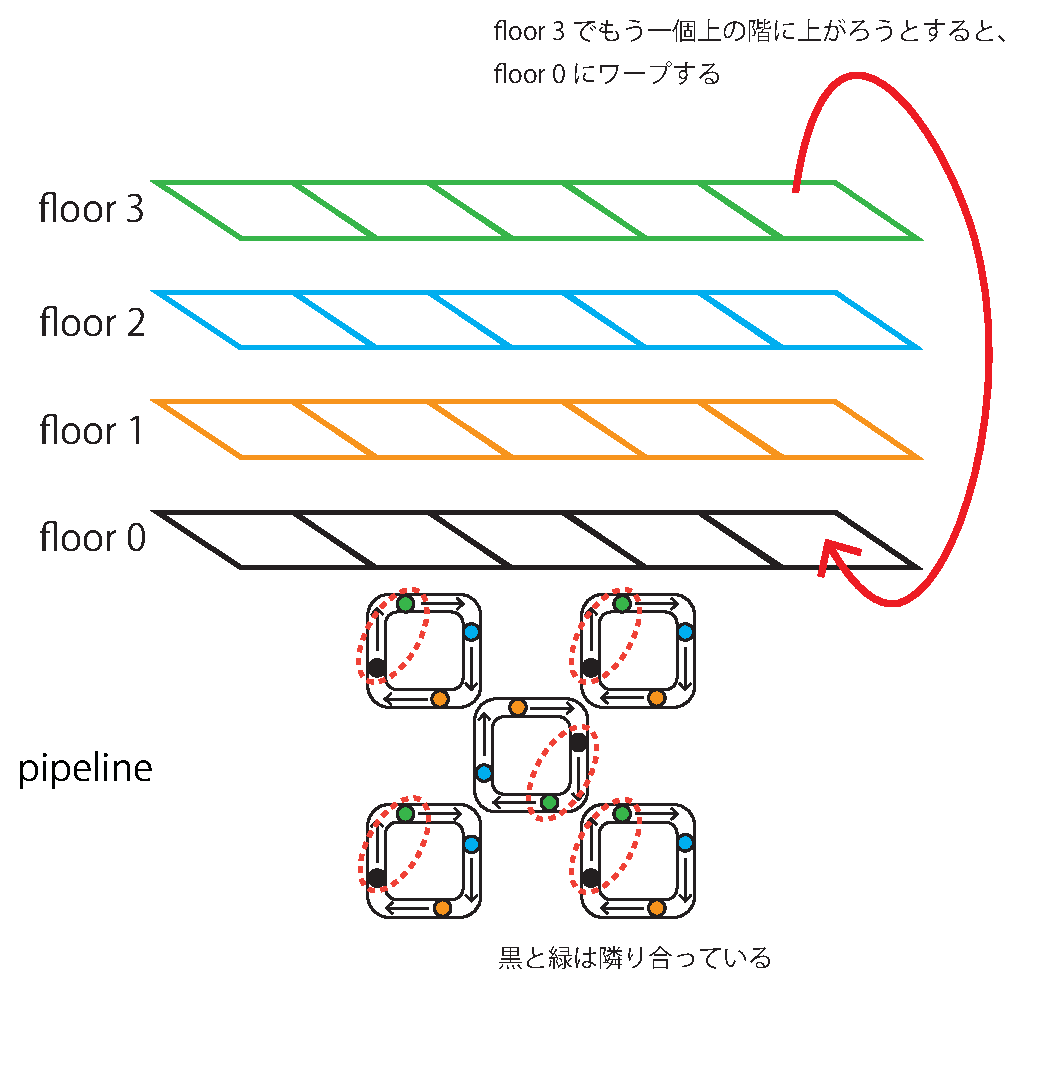
\includegraphics[scale=0.20]{figure1.eps}
    \vspace{25pt}\caption*{(a)}
    \label{}
  \end{minipage}
  \vspace{30pt}\begin{minipage}[h]{0.38\linewidth}
    \scalebox{0.45}[0.45]{
\begin{tikzpicture}[gnuplot]
%% generated with GNUPLOT 5.4p10 (Lua 5.4; terminal rev. Jun 2020, script rev. 118)
%% Sun Nov 19 18:00:22 2023
\path (0.000,0.000) rectangle (12.500,8.750);
\gpcolor{color=gp lt color border}
\gpsetlinetype{gp lt border}
\gpsetdashtype{gp dt solid}
\gpsetlinewidth{1.00}
\draw[gp path] (0.018,0.031)--(0.198,0.031);
\draw[gp path] (12.480,0.031)--(12.300,0.031);
\node[gp node right] at (-0.166,0.031) {$0$};
\draw[gp path] (0.018,0.900)--(0.198,0.900);
\draw[gp path] (12.480,0.900)--(12.300,0.900);
\node[gp node right] at (-0.166,0.900) {$5$};
\draw[gp path] (0.018,1.768)--(0.198,1.768);
\draw[gp path] (12.480,1.768)--(12.300,1.768);
\node[gp node right] at (-0.166,1.768) {$10$};
\draw[gp path] (0.018,2.637)--(0.198,2.637);
\draw[gp path] (12.480,2.637)--(12.300,2.637);
\node[gp node right] at (-0.166,2.637) {$15$};
\draw[gp path] (0.018,3.506)--(0.198,3.506);
\draw[gp path] (12.480,3.506)--(12.300,3.506);
\node[gp node right] at (-0.166,3.506) {$20$};
\draw[gp path] (0.018,4.375)--(0.198,4.375);
\draw[gp path] (12.480,4.375)--(12.300,4.375);
\node[gp node right] at (-0.166,4.375) {$25$};
\draw[gp path] (0.018,5.243)--(0.198,5.243);
\draw[gp path] (12.480,5.243)--(12.300,5.243);
\node[gp node right] at (-0.166,5.243) {$30$};
\draw[gp path] (0.018,6.112)--(0.198,6.112);
\draw[gp path] (12.480,6.112)--(12.300,6.112);
\node[gp node right] at (-0.166,6.112) {$35$};
\draw[gp path] (0.018,6.981)--(0.198,6.981);
\draw[gp path] (12.480,6.981)--(12.300,6.981);
\node[gp node right] at (-0.166,6.981) {$40$};
\draw[gp path] (0.018,7.849)--(0.198,7.849);
\draw[gp path] (12.480,7.849)--(12.300,7.849);
\node[gp node right] at (-0.166,7.849) {$45$};
\draw[gp path] (0.018,8.718)--(0.198,8.718);
\draw[gp path] (12.480,8.718)--(12.300,8.718);
\node[gp node right] at (-0.166,8.718) {$50$};
\draw[gp path] (0.018,0.031)--(0.018,0.211);
\draw[gp path] (0.018,8.718)--(0.018,8.538);
\node[gp node center] at (0.018,-0.277) {$0$};
\draw[gp path] (2.510,0.031)--(2.510,0.211);
\draw[gp path] (2.510,8.718)--(2.510,8.538);
\node[gp node center] at (2.510,-0.277) {$5$};
\draw[gp path] (5.003,0.031)--(5.003,0.211);
\draw[gp path] (5.003,8.718)--(5.003,8.538);
\node[gp node center] at (5.003,-0.277) {$10$};
\draw[gp path] (7.495,0.031)--(7.495,0.211);
\draw[gp path] (7.495,8.718)--(7.495,8.538);
\node[gp node center] at (7.495,-0.277) {$15$};
\draw[gp path] (9.988,0.031)--(9.988,0.211);
\draw[gp path] (9.988,8.718)--(9.988,8.538);
\node[gp node center] at (9.988,-0.277) {$20$};
\draw[gp path] (12.480,0.031)--(12.480,0.211);
\draw[gp path] (12.480,8.718)--(12.480,8.538);
\node[gp node center] at (12.480,-0.277) {$25$};
\draw[gp path] (0.018,8.718)--(0.018,0.031)--(12.480,0.031)--(12.480,8.718)--cycle;
\node[gp node center,rotate=-270] at (-0.826,4.374) {ボールの位置$z\ /\ \mathrm{cm}$};
\node[gp node center] at (6.249,-0.738) {時間$t\ /\ \mathrm{s}$};
\gpcolor{rgb color={0.000,0.000,0.000}}
\draw[gp path] (0.018,0.398)--(0.028,1.548)--(0.038,3.092)--(0.048,4.433)--(0.058,5.310)%
  --(0.068,5.711)--(0.078,5.854)--(0.088,5.903)--(0.098,5.899)--(0.108,5.871)--(0.118,5.838)%
  --(0.128,5.810)--(0.138,5.788)--(0.148,5.728)--(0.158,5.615)--(0.168,5.518)--(0.178,5.468)%
  --(0.187,5.352)--(0.197,5.134)--(0.207,4.990)--(0.217,4.983)--(0.227,5.025)--(0.237,5.067)%
  --(0.247,5.088)--(0.257,5.085)--(0.267,5.052)--(0.277,5.003)--(0.287,4.968)--(0.297,4.932)%
  --(0.307,4.861)--(0.317,4.800)--(0.327,4.782)--(0.337,4.790)--(0.347,4.805)--(0.357,4.805)%
  --(0.367,4.786)--(0.377,4.776)--(0.387,4.775)--(0.397,4.766)--(0.407,4.754)--(0.417,4.738)%
  --(0.427,4.725)--(0.437,4.725)--(0.447,4.729)--(0.457,4.735)--(0.467,4.740)--(0.477,4.744)%
  --(0.487,4.734)--(0.497,4.704)--(0.507,4.682)--(0.516,4.675)--(0.526,4.672)--(0.536,4.657)%
  --(0.546,4.625)--(0.556,4.604)--(0.566,4.599)--(0.576,4.598)--(0.586,4.598)--(0.596,4.599)%
  --(0.606,4.600)--(0.616,4.600)--(0.626,4.570)--(0.636,4.512)--(0.646,4.475)--(0.656,4.455)%
  --(0.666,4.463)--(0.676,4.505)--(0.686,4.548)--(0.696,4.579)--(0.706,4.598)--(0.716,4.604)%
  --(0.726,4.606)--(0.736,4.618)--(0.746,4.638)--(0.756,4.656)--(0.766,4.669)--(0.776,4.677)%
  --(0.786,4.680)--(0.796,4.680)--(0.806,4.676)--(0.816,4.665)--(0.826,4.658)--(0.836,4.658)%
  --(0.845,4.675)--(0.855,4.683)--(0.865,4.640)--(0.875,4.589)--(0.885,4.568)--(0.895,4.566)%
  --(0.905,4.570)--(0.915,4.562)--(0.925,4.335)--(0.935,3.865)--(0.945,3.612)--(0.955,3.666)%
  --(0.965,3.767)--(0.975,3.888)--(0.985,4.019)--(0.995,4.113)--(1.005,4.160)--(1.015,4.166)%
  --(1.025,4.146)--(1.035,4.113)--(1.045,4.071)--(1.055,4.031)--(1.065,4.005)--(1.075,3.995)%
  --(1.085,3.992)--(1.095,3.994)--(1.105,3.996)--(1.115,3.994)--(1.125,3.989)--(1.135,3.962)%
  --(1.145,3.911)--(1.155,3.882)--(1.165,3.884)--(1.174,3.891)--(1.184,3.895)--(1.194,3.905)%
  --(1.204,3.921)--(1.214,3.929)--(1.224,3.927)--(1.234,3.920)--(1.244,3.906)--(1.254,3.892)%
  --(1.264,3.875)--(1.274,3.848)--(1.284,3.820)--(1.294,3.798)--(1.304,3.782)--(1.314,3.774)%
  --(1.324,3.769)--(1.334,3.759)--(1.344,3.745)--(1.354,3.730)--(1.364,3.712)--(1.374,3.690)%
  --(1.384,3.667)--(1.394,3.649)--(1.404,3.628)--(1.414,3.591)--(1.424,3.560)--(1.434,3.542)%
  --(1.444,3.527)--(1.454,3.503)--(1.464,3.452)--(1.474,3.394)--(1.484,3.349)--(1.494,3.323)%
  --(1.503,3.317)--(1.513,3.324)--(1.523,3.336)--(1.533,3.344)--(1.543,3.346)--(1.553,3.335)%
  --(1.563,3.314)--(1.573,3.284)--(1.583,3.245)--(1.593,3.217)--(1.603,3.209)--(1.613,3.211)%
  --(1.623,3.216)--(1.633,3.217)--(1.643,3.219)--(1.653,3.223)--(1.663,3.224)--(1.673,3.213)%
  --(1.683,3.191)--(1.693,3.175)--(1.703,3.171)--(1.713,3.175)--(1.723,3.181)--(1.733,3.184)%
  --(1.743,3.186)--(1.753,3.184)--(1.763,3.176)--(1.773,3.162)--(1.783,3.151)--(1.793,3.153)%
  --(1.803,3.157)--(1.813,3.158)--(1.822,3.155)--(1.832,3.151)--(1.842,3.148)--(1.852,3.148)%
  --(1.862,3.152)--(1.872,3.161)--(1.882,3.172)--(1.892,3.180)--(1.902,3.186)--(1.912,3.190)%
  --(1.922,3.192)--(1.932,3.193)--(1.942,3.194)--(1.952,3.194)--(1.962,3.196)--(1.972,3.195)%
  --(1.982,3.187)--(1.992,3.178)--(2.002,3.170)--(2.012,3.164)--(2.022,3.157)--(2.032,3.153)%
  --(2.042,3.159)--(2.052,3.181)--(2.062,3.217)--(2.072,3.254)--(2.082,3.282)--(2.092,3.300)%
  --(2.102,3.314)--(2.112,3.329)--(2.122,3.342)--(2.132,3.337)--(2.142,3.311)--(2.151,3.303)%
  --(2.161,3.327)--(2.171,3.363)--(2.181,3.398)--(2.191,3.424)--(2.201,3.439)--(2.211,3.448)%
  --(2.221,3.458)--(2.231,3.468)--(2.241,3.462)--(2.251,3.435)--(2.261,3.420)--(2.271,3.430)%
  --(2.281,3.447)--(2.291,3.462)--(2.301,3.472)--(2.311,3.481)--(2.321,3.479)--(2.331,3.451)%
  --(2.341,3.403)--(2.351,3.364)--(2.361,3.345)--(2.371,3.280)--(2.381,3.143)--(2.391,3.052)%
  --(2.401,3.051)--(2.411,3.085)--(2.421,3.116)--(2.431,3.146)--(2.441,3.179)--(2.451,3.203)%
  --(2.461,3.212)--(2.471,3.209)--(2.480,3.196)--(2.490,3.170)--(2.500,3.138)--(2.510,3.120)%
  --(2.520,3.119)--(2.530,3.127)--(2.540,3.138)--(2.550,3.146)--(2.560,3.156)--(2.570,3.165)%
  --(2.580,3.168)--(2.590,3.168)--(2.600,3.171)--(2.610,3.170)--(2.620,3.164)--(2.630,3.159)%
  --(2.640,3.144)--(2.650,3.119)--(2.660,3.113)--(2.670,3.130)--(2.680,3.152)--(2.690,3.177)%
  --(2.700,3.201)--(2.710,3.213)--(2.720,3.212)--(2.730,3.200)--(2.740,3.188)--(2.750,3.182)%
  --(2.760,3.180)--(2.770,3.181)--(2.780,3.189)--(2.790,3.190)--(2.800,3.178)--(2.809,3.180)%
  --(2.819,3.209)--(2.829,3.246)--(2.839,3.273)--(2.849,3.279)--(2.859,3.258)--(2.869,3.232)%
  --(2.879,3.239)--(2.889,3.279)--(2.899,3.329)--(2.909,3.379)--(2.919,3.425)--(2.929,3.463)%
  --(2.939,3.491)--(2.949,3.513)--(2.959,3.532)--(2.969,3.552)--(2.979,3.581)--(2.989,3.619)%
  --(2.999,3.656)--(3.009,3.691)--(3.019,3.716)--(3.029,3.729)--(3.039,3.732)--(3.049,3.731)%
  --(3.059,3.725)--(3.069,3.712)--(3.079,3.696)--(3.089,3.680)--(3.099,3.655)--(3.109,3.616)%
  --(3.119,3.573)--(3.129,3.514)--(3.138,3.432)--(3.148,3.364)--(3.158,3.314)--(3.168,3.264)%
  --(3.178,3.207)--(3.188,3.145)--(3.198,3.092)--(3.208,3.046)--(3.218,2.993)--(3.228,2.933)%
  --(3.238,2.871)--(3.248,2.806)--(3.258,2.730)--(3.268,2.653)--(3.278,2.587)--(3.288,2.536)%
  --(3.298,2.498)--(3.308,2.475)--(3.318,2.455)--(3.328,2.429)--(3.338,2.404)--(3.348,2.378)%
  --(3.358,2.356)--(3.368,2.359)--(3.378,2.386)--(3.388,2.425)--(3.398,2.440)--(3.408,2.419)%
  --(3.418,2.433)--(3.428,2.501)--(3.438,2.582)--(3.448,2.662)--(3.458,2.736)--(3.467,2.809)%
  --(3.477,2.881)--(3.487,2.898)--(3.497,2.863)--(3.507,2.892)--(3.517,3.008)--(3.527,3.141)%
  --(3.537,3.269)--(3.547,3.397)--(3.557,3.512)--(3.567,3.606)--(3.577,3.683)--(3.587,3.749)%
  --(3.597,3.801)--(3.607,3.837)--(3.617,3.867)--(3.627,3.901)--(3.637,3.927)--(3.647,3.935)%
  --(3.657,3.882)--(3.667,3.772)--(3.677,3.736)--(3.687,3.801)--(3.697,3.884)--(3.707,3.951)%
  --(3.717,3.990)--(3.727,3.995)--(3.737,3.974)--(3.747,3.942)--(3.757,3.904)--(3.767,3.872)%
  --(3.777,3.854)--(3.787,3.827)--(3.796,3.773)--(3.806,3.692)--(3.816,3.579)--(3.826,3.459)%
  --(3.836,3.375)--(3.846,3.328)--(3.856,3.297)--(3.866,3.270)--(3.876,3.240)--(3.886,3.207)%
  --(3.896,3.178)--(3.906,3.154)--(3.916,3.129)--(3.926,3.104)--(3.936,3.085)--(3.946,3.071)%
  --(3.956,3.043)--(3.966,3.002)--(3.976,2.979)--(3.986,2.983)--(3.996,2.995)--(4.006,3.006)%
  --(4.016,3.014)--(4.026,2.974)--(4.036,2.877)--(4.046,2.835)--(4.056,2.879)--(4.066,2.948)%
  --(4.076,3.008)--(4.086,3.067)--(4.096,3.126)--(4.106,3.177)--(4.116,3.218)--(4.125,3.254)%
  --(4.135,3.287)--(4.145,3.313)--(4.155,3.323)--(4.165,3.350)--(4.175,3.437)--(4.185,3.559)%
  --(4.195,3.668)--(4.205,3.749)--(4.215,3.791)--(4.225,3.800)--(4.235,3.810)--(4.245,3.817)%
  --(4.255,3.803)--(4.265,3.799)--(4.275,3.814)--(4.285,3.829)--(4.295,3.838)--(4.305,3.822)%
  --(4.315,3.775)--(4.325,3.732)--(4.335,3.710)--(4.345,3.689)--(4.355,3.639)--(4.365,3.538)%
  --(4.375,3.408)--(4.385,3.291)--(4.395,3.208)--(4.405,3.133)--(4.415,3.042)--(4.425,2.936)%
  --(4.435,2.836)--(4.445,2.752)--(4.454,2.677)--(4.464,2.608)--(4.474,2.544)--(4.484,2.475)%
  --(4.494,2.397)--(4.504,2.330)--(4.514,2.289)--(4.524,2.259)--(4.534,2.225)--(4.544,2.197)%
  --(4.554,2.175)--(4.564,2.156)--(4.574,2.142)--(4.584,2.132)--(4.594,2.119)--(4.604,2.100)%
  --(4.614,2.073)--(4.624,2.057)--(4.634,2.060)--(4.644,2.073)--(4.654,2.089)--(4.664,2.109)%
  --(4.674,2.135)--(4.684,2.168)--(4.694,2.202)--(4.704,2.234)--(4.714,2.266)--(4.724,2.293)%
  --(4.734,2.324)--(4.744,2.384)--(4.754,2.466)--(4.764,2.544)--(4.773,2.601)--(4.783,2.633)%
  --(4.793,2.660)--(4.803,2.690)--(4.813,2.691)--(4.823,2.649)--(4.833,2.609)--(4.843,2.588)%
  --(4.853,2.565)--(4.863,2.529)--(4.873,2.480)--(4.883,2.419)--(4.893,2.347)--(4.903,2.267)%
  --(4.913,2.182)--(4.923,2.093)--(4.933,2.003)--(4.943,1.915)--(4.953,1.831)--(4.963,1.748)%
  --(4.973,1.665)--(4.983,1.590)--(4.993,1.521)--(5.003,1.460)--(5.013,1.416)--(5.023,1.385)%
  --(5.033,1.363)--(5.043,1.355)--(5.053,1.358)--(5.063,1.368)--(5.073,1.382)--(5.083,1.403)%
  --(5.093,1.434)--(5.102,1.478)--(5.112,1.534)--(5.122,1.598)--(5.132,1.668)--(5.142,1.730)%
  --(5.152,1.779)--(5.162,1.822)--(5.172,1.856)--(5.182,1.875)--(5.192,1.873)--(5.202,1.848)%
  --(5.212,1.793)--(5.222,1.704)--(5.232,1.605)--(5.242,1.520)--(5.252,1.459)--(5.262,1.424)%
  --(5.272,1.405)--(5.282,1.391)--(5.292,1.380)--(5.302,1.386)--(5.312,1.440)--(5.322,1.544)%
  --(5.332,1.670)--(5.342,1.817)--(5.352,1.986)--(5.362,2.169)--(5.372,2.338)--(5.382,2.464)%
  --(5.392,2.549)--(5.402,2.606)--(5.412,2.642)--(5.422,2.666)--(5.431,2.685)--(5.441,2.699)%
  --(5.451,2.709)--(5.461,2.706)--(5.471,2.682)--(5.481,2.649)--(5.491,2.621)--(5.501,2.608)%
  --(5.511,2.617)--(5.521,2.637)--(5.531,2.660)--(5.541,2.662)--(5.551,2.636)--(5.561,2.621)%
  --(5.571,2.632)--(5.581,2.657)--(5.591,2.686)--(5.601,2.707)--(5.611,2.714)--(5.621,2.718)%
  --(5.631,2.722)--(5.641,2.717)--(5.651,2.707)--(5.661,2.701)--(5.671,2.698)--(5.681,2.687)%
  --(5.691,2.663)--(5.701,2.640)--(5.711,2.628)--(5.721,2.625)--(5.731,2.626)--(5.741,2.624)%
  --(5.751,2.617)--(5.760,2.606)--(5.770,2.590)--(5.780,2.571)--(5.790,2.553)--(5.800,2.532)%
  --(5.810,2.516)--(5.820,2.507)--(5.830,2.478)--(5.840,2.415)--(5.850,2.329)--(5.860,2.232)%
  --(5.870,2.134)--(5.880,2.040)--(5.890,1.948)--(5.900,1.860)--(5.910,1.771)--(5.920,1.676)%
  --(5.930,1.579)--(5.940,1.489)--(5.950,1.427)--(5.960,1.401)--(5.970,1.410)--(5.980,1.450)%
  --(5.990,1.513)--(6.000,1.583)--(6.010,1.651)--(6.020,1.726)--(6.030,1.810)--(6.040,1.902)%
  --(6.050,2.001)--(6.060,2.104)--(6.070,2.212)--(6.080,2.316)--(6.089,2.413)--(6.099,2.507)%
  --(6.109,2.592)--(6.119,2.662)--(6.129,2.735)--(6.139,2.817)--(6.149,2.899)--(6.159,2.956)%
  --(6.169,2.971)--(6.179,2.969)--(6.189,2.976)--(6.199,3.010)--(6.209,3.066)--(6.219,3.112)%
  --(6.229,3.137)--(6.239,3.154)--(6.249,3.163)--(6.259,3.153)--(6.269,3.141)--(6.279,3.137)%
  --(6.289,3.136)--(6.299,3.128)--(6.309,3.110)--(6.319,3.084)--(6.329,3.043)--(6.339,2.991)%
  --(6.349,2.939)--(6.359,2.893)--(6.369,2.855)--(6.379,2.826)--(6.389,2.804)--(6.399,2.788)%
  --(6.409,2.778)--(6.418,2.772)--(6.428,2.766)--(6.438,2.770)--(6.448,2.794)--(6.458,2.829)%
  --(6.468,2.866)--(6.478,2.902)--(6.488,2.937)--(6.498,2.964)--(6.508,2.978)--(6.518,2.985)%
  --(6.528,2.993)--(6.538,3.029)--(6.548,3.091)--(6.558,3.170)--(6.568,3.263)--(6.578,3.360)%
  --(6.588,3.456)--(6.598,3.551)--(6.608,3.641)--(6.618,3.726)--(6.628,3.803)--(6.638,3.859)%
  --(6.648,3.888)--(6.658,3.903)--(6.668,3.927)--(6.678,3.975)--(6.688,4.034)--(6.698,4.056)%
  --(6.708,4.031)--(6.718,4.008)--(6.728,3.988)--(6.738,3.947)--(6.747,3.919)--(6.757,3.803)%
  --(6.767,3.563)--(6.777,3.436)--(6.787,3.496)--(6.797,3.604)--(6.807,3.689)--(6.817,3.741)%
  --(6.827,3.762)--(6.837,3.761)--(6.847,3.751)--(6.857,3.726)--(6.867,3.688)--(6.877,3.674)%
  --(6.887,3.701)--(6.897,3.740)--(6.907,3.772)--(6.917,3.804)--(6.927,3.837)--(6.937,3.873)%
  --(6.947,3.914)--(6.957,3.940)--(6.967,3.931)--(6.977,3.923)--(6.987,3.950)--(6.997,4.010)%
  --(7.007,4.086)--(7.017,4.163)--(7.027,4.236)--(7.037,4.301)--(7.047,4.351)--(7.057,4.379)%
  --(7.067,4.392)--(7.076,4.393)--(7.086,4.386)--(7.096,4.391)--(7.106,4.411)--(7.116,4.408)%
  --(7.126,4.358)--(7.136,4.279)--(7.146,4.222)--(7.156,4.198)--(7.166,4.176)--(7.176,4.136)%
  --(7.186,4.075)--(7.196,4.001)--(7.206,3.930)--(7.216,3.866)--(7.226,3.800)--(7.236,3.729)%
  --(7.246,3.656)--(7.256,3.582)--(7.266,3.512)--(7.276,3.448)--(7.286,3.392)--(7.296,3.351)%
  --(7.306,3.327)--(7.316,3.309)--(7.326,3.289)--(7.336,3.274)--(7.346,3.267)--(7.356,3.259)%
  --(7.366,3.238)--(7.376,3.206)--(7.386,3.187)--(7.396,3.187)--(7.405,3.197)--(7.415,3.211)%
  --(7.425,3.223)--(7.435,3.231)--(7.445,3.245)--(7.455,3.271)--(7.465,3.307)--(7.475,3.346)%
  --(7.485,3.397)--(7.495,3.475)--(7.505,3.567)--(7.515,3.644)--(7.525,3.694)--(7.535,3.736)%
  --(7.545,3.784)--(7.555,3.827)--(7.565,3.860)--(7.575,3.881)--(7.585,3.894)--(7.595,3.899)%
  --(7.605,3.898)--(7.615,3.893)--(7.625,3.877)--(7.635,3.850)--(7.645,3.801)--(7.655,3.732)%
  --(7.665,3.678)--(7.675,3.648)--(7.685,3.623)--(7.695,3.595)--(7.705,3.559)--(7.715,3.523)%
  --(7.725,3.492)--(7.734,3.461)--(7.744,3.429)--(7.754,3.410)--(7.764,3.406)--(7.774,3.413)%
  --(7.784,3.413)--(7.794,3.402)--(7.804,3.398)--(7.814,3.406)--(7.824,3.417)--(7.834,3.427)%
  --(7.844,3.435)--(7.854,3.439)--(7.864,3.432)--(7.874,3.415)--(7.884,3.400)--(7.894,3.394)%
  --(7.904,3.419)--(7.914,3.476)--(7.924,3.543)--(7.934,3.609)--(7.944,3.674)--(7.954,3.738)%
  --(7.964,3.788)--(7.974,3.802)--(7.984,3.789)--(7.994,3.791)--(8.004,3.823)--(8.014,3.870)%
  --(8.024,3.920)--(8.034,3.951)--(8.044,3.952)--(8.053,3.948)--(8.063,3.950)--(8.073,3.947)%
  --(8.083,3.933)--(8.093,3.891)--(8.103,3.815)--(8.113,3.746)--(8.123,3.707)--(8.133,3.684)%
  --(8.143,3.668)--(8.153,3.653)--(8.163,3.638)--(8.173,3.626)--(8.183,3.620)--(8.193,3.632)%
  --(8.203,3.656)--(8.213,3.668)--(8.223,3.662)--(8.233,3.646)--(8.243,3.623)--(8.253,3.599)%
  --(8.263,3.569)--(8.273,3.529)--(8.283,3.476)--(8.293,3.412)--(8.303,3.363)--(8.313,3.344)%
  --(8.323,3.334)--(8.333,3.318)--(8.343,3.295)--(8.353,3.270)--(8.363,3.247)--(8.373,3.218)%
  --(8.382,3.178)--(8.392,3.149)--(8.402,3.143)--(8.412,3.171)--(8.422,3.220)--(8.432,3.267)%
  --(8.442,3.308)--(8.452,3.341)--(8.462,3.367)--(8.472,3.386)--(8.482,3.385)--(8.492,3.358)%
  --(8.502,3.326)--(8.512,3.292)--(8.522,3.248)--(8.532,3.213)--(8.542,3.196)--(8.552,3.166)%
  --(8.562,3.111)--(8.572,3.059)--(8.582,3.007)--(8.592,2.935)--(8.602,2.846)--(8.612,2.743)%
  --(8.622,2.634)--(8.632,2.518)--(8.642,2.396)--(8.652,2.267)--(8.662,2.134)--(8.672,2.001)%
  --(8.682,1.867)--(8.692,1.727)--(8.702,1.589)--(8.711,1.492)--(8.721,1.456)--(8.731,1.494)%
  --(8.741,1.615)--(8.751,1.792)--(8.761,1.987)--(8.771,2.160)--(8.781,2.291)--(8.791,2.396)%
  --(8.801,2.477)--(8.811,2.532)--(8.821,2.572)--(8.831,2.608)--(8.841,2.636)--(8.851,2.655)%
  --(8.861,2.668)--(8.871,2.677)--(8.881,2.679)--(8.891,2.678)--(8.901,2.674)--(8.911,2.655)%
  --(8.921,2.614)--(8.931,2.555)--(8.941,2.486)--(8.951,2.440)--(8.961,2.432)--(8.971,2.432)%
  --(8.981,2.424)--(8.991,2.425)--(9.001,2.441)--(9.011,2.462)--(9.021,2.481)--(9.031,2.500)%
  --(9.040,2.524)--(9.050,2.548)--(9.060,2.570)--(9.070,2.597)--(9.080,2.630)--(9.090,2.658)%
  --(9.100,2.681)--(9.110,2.699)--(9.120,2.709)--(9.130,2.713)--(9.140,2.713)--(9.150,2.711)%
  --(9.160,2.698)--(9.170,2.675)--(9.180,2.657)--(9.190,2.649)--(9.200,2.646)--(9.210,2.643)%
  --(9.220,2.638)--(9.230,2.633)--(9.240,2.625)--(9.250,2.610)--(9.260,2.588)--(9.270,2.564)%
  --(9.280,2.542)--(9.290,2.526)--(9.300,2.517)--(9.310,2.493)--(9.320,2.422)--(9.330,2.311)%
  --(9.340,2.197)--(9.350,2.094)--(9.360,1.994)--(9.369,1.888)--(9.379,1.770)--(9.389,1.648)%
  --(9.399,1.539)--(9.409,1.456)--(9.419,1.417)--(9.429,1.424)--(9.439,1.468)--(9.449,1.537)%
  --(9.459,1.622)--(9.469,1.713)--(9.479,1.802)--(9.489,1.898)--(9.499,2.002)--(9.509,2.106)%
  --(9.519,2.209)--(9.529,2.326)--(9.539,2.474)--(9.549,2.640)--(9.559,2.784)--(9.569,2.878)%
  --(9.579,2.934)--(9.589,2.992)--(9.599,3.068)--(9.609,3.149)--(9.619,3.225)--(9.629,3.296)%
  --(9.639,3.371)--(9.649,3.450)--(9.659,3.526)--(9.669,3.578)--(9.679,3.590)--(9.689,3.595)%
  --(9.698,3.613)--(9.708,3.618)--(9.718,3.600)--(9.728,3.595)--(9.738,3.609)--(9.748,3.621)%
  --(9.758,3.621)--(9.768,3.602)--(9.778,3.568)--(9.788,3.516)--(9.798,3.440)--(9.808,3.373)%
  --(9.818,3.333)--(9.828,3.301)--(9.838,3.270)--(9.848,3.238)--(9.858,3.192)--(9.868,3.129)%
  --(9.878,3.081)--(9.888,3.058)--(9.898,3.050)--(9.908,3.044)--(9.918,3.038)--(9.928,3.034)%
  --(9.938,3.023)--(9.948,3.004)--(9.958,3.001)--(9.968,3.018)--(9.978,3.040)--(9.988,3.065)%
  --(9.998,3.098)--(10.008,3.131)--(10.018,3.156)--(10.027,3.177)--(10.037,3.206)--(10.047,3.248)%
  --(10.057,3.302)--(10.067,3.364)--(10.077,3.432)--(10.087,3.501)--(10.097,3.573)--(10.107,3.647)%
  --(10.117,3.716)--(10.127,3.774)--(10.137,3.825)--(10.147,3.878)--(10.157,3.926)--(10.167,3.963)%
  --(10.177,3.993)--(10.187,4.019)--(10.197,4.041)--(10.207,4.057)--(10.217,4.062)--(10.227,4.051)%
  --(10.237,4.024)--(10.247,3.988)--(10.257,3.945)--(10.267,3.892)--(10.277,3.840)--(10.287,3.797)%
  --(10.297,3.763)--(10.307,3.731)--(10.317,3.694)--(10.327,3.652)--(10.337,3.599)--(10.347,3.528)%
  --(10.356,3.471)--(10.366,3.463)--(10.376,3.487)--(10.386,3.520)--(10.396,3.558)--(10.406,3.593)%
  --(10.416,3.616)--(10.426,3.627)--(10.436,3.630)--(10.446,3.623)--(10.456,3.615)--(10.466,3.635)%
  --(10.476,3.684)--(10.486,3.739)--(10.496,3.775)--(10.506,3.792)--(10.516,3.831)--(10.526,3.897)%
  --(10.536,3.977)--(10.546,4.058)--(10.556,4.134)--(10.566,4.204)--(10.576,4.272)--(10.586,4.339)%
  --(10.596,4.408)--(10.606,4.476)--(10.616,4.540)--(10.626,4.585)--(10.636,4.613)--(10.646,4.642)%
  --(10.656,4.655)--(10.666,4.637)--(10.676,4.638)--(10.685,4.669)--(10.695,4.692)--(10.705,4.724)%
  --(10.715,4.770)--(10.725,4.795)--(10.735,4.775)--(10.745,4.727)--(10.755,4.680)--(10.765,4.633)%
  --(10.775,4.564)--(10.785,4.498)--(10.795,4.488)--(10.805,4.531)--(10.815,4.585)--(10.825,4.627)%
  --(10.835,4.611)--(10.845,4.543)--(10.855,4.520)--(10.865,4.569)--(10.875,4.642)--(10.885,4.716)%
  --(10.895,4.781)--(10.905,4.832)--(10.915,4.875)--(10.925,4.918)--(10.935,4.964)--(10.945,5.008)%
  --(10.955,5.047)--(10.965,5.042)--(10.975,4.993)--(10.985,4.988)--(10.995,5.037)--(11.004,5.093)%
  --(11.014,5.170)--(11.024,5.252)--(11.034,5.301)--(11.044,5.322)--(11.054,5.336)--(11.064,5.353)%
  --(11.074,5.370)--(11.084,5.376)--(11.094,5.357)--(11.104,5.316)--(11.114,5.275)--(11.124,5.240)%
  --(11.134,5.207)--(11.144,5.173)--(11.154,4.972)--(11.164,4.577)--(11.174,4.350)--(11.184,4.378)%
  --(11.194,4.478)--(11.204,4.601)--(11.214,4.707)--(11.224,4.744)--(11.234,4.725)--(11.244,4.678)%
  --(11.254,4.623)--(11.264,4.573)--(11.274,4.534)--(11.284,4.499)--(11.294,4.460)--(11.304,4.420)%
  --(11.314,4.412)--(11.324,4.437)--(11.333,4.471)--(11.343,4.482)--(11.353,4.464)--(11.363,4.463)%
  --(11.373,4.450)--(11.383,4.404)--(11.393,4.410)--(11.403,4.486)--(11.413,4.581)--(11.423,4.674)%
  --(11.433,4.778)--(11.443,4.892)--(11.453,4.982)--(11.463,5.006)--(11.473,4.979)--(11.483,4.983)%
  --(11.493,5.048)--(11.503,5.147)--(11.513,5.247)--(11.523,5.324)--(11.533,5.377)--(11.543,5.421)%
  --(11.553,5.459)--(11.563,5.501)--(11.573,5.543)--(11.583,5.554)--(11.593,5.513)--(11.603,5.450)%
  --(11.613,5.430)--(11.623,5.452)--(11.633,5.462)--(11.643,5.433)--(11.653,5.390)--(11.662,5.374)%
  --(11.672,5.362)--(11.682,5.311)--(11.692,5.236)--(11.702,5.185)--(11.712,5.160)--(11.722,5.140)%
  --(11.732,5.116)--(11.742,5.067)--(11.752,4.995)--(11.762,4.923)--(11.772,4.865)--(11.782,4.835)%
  --(11.792,4.806)--(11.802,4.759)--(11.812,4.743)--(11.822,4.787)--(11.832,4.864)--(11.842,4.923)%
  --(11.852,4.946)--(11.862,4.948)--(11.872,4.941)--(11.882,4.935)--(11.892,4.943)--(11.902,4.963)%
  --(11.912,4.987)--(11.922,5.012)--(11.932,5.054)--(11.942,5.104)--(11.952,5.146)--(11.962,5.201)%
  --(11.972,5.283)--(11.982,5.382)--(11.991,5.472)--(12.001,5.534)--(12.011,5.577)--(12.021,5.617)%
  --(12.031,5.659)--(12.041,5.706)--(12.051,5.757)--(12.061,5.811)--(12.071,5.858)--(12.081,5.879)%
  --(12.091,5.835)--(12.101,5.743)--(12.111,5.707)--(12.121,5.755)--(12.131,5.843)--(12.141,5.928)%
  --(12.151,5.993)--(12.161,6.038)--(12.171,6.055)--(12.181,6.045)--(12.191,6.006)--(12.201,5.944)%
  --(12.211,5.890)--(12.221,5.881)--(12.231,5.913)--(12.241,5.968)--(12.251,6.018)--(12.261,6.043)%
  --(12.271,6.051)--(12.281,6.058)--(12.291,6.096)--(12.301,6.172)--(12.311,6.273)--(12.320,6.385)%
  --(12.330,6.498)--(12.340,6.623)--(12.350,6.742)--(12.360,6.830)--(12.370,6.885)--(12.380,6.909)%
  --(12.390,6.932)--(12.400,6.992)--(12.410,7.183)--(12.420,7.552)--(12.430,7.957)--(12.440,8.251)%
  --(12.450,8.420)--(12.460,8.577)--(12.470,8.704)--(12.480,8.683);
\gpsetpointsize{1.20}
\gp3point{gp mark 7}{}{(0.018,0.398)}
\gp3point{gp mark 7}{}{(0.028,1.548)}
\gp3point{gp mark 7}{}{(0.038,3.092)}
\gp3point{gp mark 7}{}{(0.048,4.433)}
\gp3point{gp mark 7}{}{(0.058,5.310)}
\gp3point{gp mark 7}{}{(0.068,5.711)}
\gp3point{gp mark 7}{}{(0.078,5.854)}
\gp3point{gp mark 7}{}{(0.088,5.903)}
\gp3point{gp mark 7}{}{(0.098,5.899)}
\gp3point{gp mark 7}{}{(0.108,5.871)}
\gp3point{gp mark 7}{}{(0.118,5.838)}
\gp3point{gp mark 7}{}{(0.128,5.810)}
\gp3point{gp mark 7}{}{(0.138,5.788)}
\gp3point{gp mark 7}{}{(0.148,5.728)}
\gp3point{gp mark 7}{}{(0.158,5.615)}
\gp3point{gp mark 7}{}{(0.168,5.518)}
\gp3point{gp mark 7}{}{(0.178,5.468)}
\gp3point{gp mark 7}{}{(0.187,5.352)}
\gp3point{gp mark 7}{}{(0.197,5.134)}
\gp3point{gp mark 7}{}{(0.207,4.990)}
\gp3point{gp mark 7}{}{(0.217,4.983)}
\gp3point{gp mark 7}{}{(0.227,5.025)}
\gp3point{gp mark 7}{}{(0.237,5.067)}
\gp3point{gp mark 7}{}{(0.247,5.088)}
\gp3point{gp mark 7}{}{(0.257,5.085)}
\gp3point{gp mark 7}{}{(0.267,5.052)}
\gp3point{gp mark 7}{}{(0.277,5.003)}
\gp3point{gp mark 7}{}{(0.287,4.968)}
\gp3point{gp mark 7}{}{(0.297,4.932)}
\gp3point{gp mark 7}{}{(0.307,4.861)}
\gp3point{gp mark 7}{}{(0.317,4.800)}
\gp3point{gp mark 7}{}{(0.327,4.782)}
\gp3point{gp mark 7}{}{(0.337,4.790)}
\gp3point{gp mark 7}{}{(0.347,4.805)}
\gp3point{gp mark 7}{}{(0.357,4.805)}
\gp3point{gp mark 7}{}{(0.367,4.786)}
\gp3point{gp mark 7}{}{(0.377,4.776)}
\gp3point{gp mark 7}{}{(0.387,4.775)}
\gp3point{gp mark 7}{}{(0.397,4.766)}
\gp3point{gp mark 7}{}{(0.407,4.754)}
\gp3point{gp mark 7}{}{(0.417,4.738)}
\gp3point{gp mark 7}{}{(0.427,4.725)}
\gp3point{gp mark 7}{}{(0.437,4.725)}
\gp3point{gp mark 7}{}{(0.447,4.729)}
\gp3point{gp mark 7}{}{(0.457,4.735)}
\gp3point{gp mark 7}{}{(0.467,4.740)}
\gp3point{gp mark 7}{}{(0.477,4.744)}
\gp3point{gp mark 7}{}{(0.487,4.734)}
\gp3point{gp mark 7}{}{(0.497,4.704)}
\gp3point{gp mark 7}{}{(0.507,4.682)}
\gp3point{gp mark 7}{}{(0.516,4.675)}
\gp3point{gp mark 7}{}{(0.526,4.672)}
\gp3point{gp mark 7}{}{(0.536,4.657)}
\gp3point{gp mark 7}{}{(0.546,4.625)}
\gp3point{gp mark 7}{}{(0.556,4.604)}
\gp3point{gp mark 7}{}{(0.566,4.599)}
\gp3point{gp mark 7}{}{(0.576,4.598)}
\gp3point{gp mark 7}{}{(0.586,4.598)}
\gp3point{gp mark 7}{}{(0.596,4.599)}
\gp3point{gp mark 7}{}{(0.606,4.600)}
\gp3point{gp mark 7}{}{(0.616,4.600)}
\gp3point{gp mark 7}{}{(0.626,4.570)}
\gp3point{gp mark 7}{}{(0.636,4.512)}
\gp3point{gp mark 7}{}{(0.646,4.475)}
\gp3point{gp mark 7}{}{(0.656,4.455)}
\gp3point{gp mark 7}{}{(0.666,4.463)}
\gp3point{gp mark 7}{}{(0.676,4.505)}
\gp3point{gp mark 7}{}{(0.686,4.548)}
\gp3point{gp mark 7}{}{(0.696,4.579)}
\gp3point{gp mark 7}{}{(0.706,4.598)}
\gp3point{gp mark 7}{}{(0.716,4.604)}
\gp3point{gp mark 7}{}{(0.726,4.606)}
\gp3point{gp mark 7}{}{(0.736,4.618)}
\gp3point{gp mark 7}{}{(0.746,4.638)}
\gp3point{gp mark 7}{}{(0.756,4.656)}
\gp3point{gp mark 7}{}{(0.766,4.669)}
\gp3point{gp mark 7}{}{(0.776,4.677)}
\gp3point{gp mark 7}{}{(0.786,4.680)}
\gp3point{gp mark 7}{}{(0.796,4.680)}
\gp3point{gp mark 7}{}{(0.806,4.676)}
\gp3point{gp mark 7}{}{(0.816,4.665)}
\gp3point{gp mark 7}{}{(0.826,4.658)}
\gp3point{gp mark 7}{}{(0.836,4.658)}
\gp3point{gp mark 7}{}{(0.845,4.675)}
\gp3point{gp mark 7}{}{(0.855,4.683)}
\gp3point{gp mark 7}{}{(0.865,4.640)}
\gp3point{gp mark 7}{}{(0.875,4.589)}
\gp3point{gp mark 7}{}{(0.885,4.568)}
\gp3point{gp mark 7}{}{(0.895,4.566)}
\gp3point{gp mark 7}{}{(0.905,4.570)}
\gp3point{gp mark 7}{}{(0.915,4.562)}
\gp3point{gp mark 7}{}{(0.925,4.335)}
\gp3point{gp mark 7}{}{(0.935,3.865)}
\gp3point{gp mark 7}{}{(0.945,3.612)}
\gp3point{gp mark 7}{}{(0.955,3.666)}
\gp3point{gp mark 7}{}{(0.965,3.767)}
\gp3point{gp mark 7}{}{(0.975,3.888)}
\gp3point{gp mark 7}{}{(0.985,4.019)}
\gp3point{gp mark 7}{}{(0.995,4.113)}
\gp3point{gp mark 7}{}{(1.005,4.160)}
\gp3point{gp mark 7}{}{(1.015,4.166)}
\gp3point{gp mark 7}{}{(1.025,4.146)}
\gp3point{gp mark 7}{}{(1.035,4.113)}
\gp3point{gp mark 7}{}{(1.045,4.071)}
\gp3point{gp mark 7}{}{(1.055,4.031)}
\gp3point{gp mark 7}{}{(1.065,4.005)}
\gp3point{gp mark 7}{}{(1.075,3.995)}
\gp3point{gp mark 7}{}{(1.085,3.992)}
\gp3point{gp mark 7}{}{(1.095,3.994)}
\gp3point{gp mark 7}{}{(1.105,3.996)}
\gp3point{gp mark 7}{}{(1.115,3.994)}
\gp3point{gp mark 7}{}{(1.125,3.989)}
\gp3point{gp mark 7}{}{(1.135,3.962)}
\gp3point{gp mark 7}{}{(1.145,3.911)}
\gp3point{gp mark 7}{}{(1.155,3.882)}
\gp3point{gp mark 7}{}{(1.165,3.884)}
\gp3point{gp mark 7}{}{(1.174,3.891)}
\gp3point{gp mark 7}{}{(1.184,3.895)}
\gp3point{gp mark 7}{}{(1.194,3.905)}
\gp3point{gp mark 7}{}{(1.204,3.921)}
\gp3point{gp mark 7}{}{(1.214,3.929)}
\gp3point{gp mark 7}{}{(1.224,3.927)}
\gp3point{gp mark 7}{}{(1.234,3.920)}
\gp3point{gp mark 7}{}{(1.244,3.906)}
\gp3point{gp mark 7}{}{(1.254,3.892)}
\gp3point{gp mark 7}{}{(1.264,3.875)}
\gp3point{gp mark 7}{}{(1.274,3.848)}
\gp3point{gp mark 7}{}{(1.284,3.820)}
\gp3point{gp mark 7}{}{(1.294,3.798)}
\gp3point{gp mark 7}{}{(1.304,3.782)}
\gp3point{gp mark 7}{}{(1.314,3.774)}
\gp3point{gp mark 7}{}{(1.324,3.769)}
\gp3point{gp mark 7}{}{(1.334,3.759)}
\gp3point{gp mark 7}{}{(1.344,3.745)}
\gp3point{gp mark 7}{}{(1.354,3.730)}
\gp3point{gp mark 7}{}{(1.364,3.712)}
\gp3point{gp mark 7}{}{(1.374,3.690)}
\gp3point{gp mark 7}{}{(1.384,3.667)}
\gp3point{gp mark 7}{}{(1.394,3.649)}
\gp3point{gp mark 7}{}{(1.404,3.628)}
\gp3point{gp mark 7}{}{(1.414,3.591)}
\gp3point{gp mark 7}{}{(1.424,3.560)}
\gp3point{gp mark 7}{}{(1.434,3.542)}
\gp3point{gp mark 7}{}{(1.444,3.527)}
\gp3point{gp mark 7}{}{(1.454,3.503)}
\gp3point{gp mark 7}{}{(1.464,3.452)}
\gp3point{gp mark 7}{}{(1.474,3.394)}
\gp3point{gp mark 7}{}{(1.484,3.349)}
\gp3point{gp mark 7}{}{(1.494,3.323)}
\gp3point{gp mark 7}{}{(1.503,3.317)}
\gp3point{gp mark 7}{}{(1.513,3.324)}
\gp3point{gp mark 7}{}{(1.523,3.336)}
\gp3point{gp mark 7}{}{(1.533,3.344)}
\gp3point{gp mark 7}{}{(1.543,3.346)}
\gp3point{gp mark 7}{}{(1.553,3.335)}
\gp3point{gp mark 7}{}{(1.563,3.314)}
\gp3point{gp mark 7}{}{(1.573,3.284)}
\gp3point{gp mark 7}{}{(1.583,3.245)}
\gp3point{gp mark 7}{}{(1.593,3.217)}
\gp3point{gp mark 7}{}{(1.603,3.209)}
\gp3point{gp mark 7}{}{(1.613,3.211)}
\gp3point{gp mark 7}{}{(1.623,3.216)}
\gp3point{gp mark 7}{}{(1.633,3.217)}
\gp3point{gp mark 7}{}{(1.643,3.219)}
\gp3point{gp mark 7}{}{(1.653,3.223)}
\gp3point{gp mark 7}{}{(1.663,3.224)}
\gp3point{gp mark 7}{}{(1.673,3.213)}
\gp3point{gp mark 7}{}{(1.683,3.191)}
\gp3point{gp mark 7}{}{(1.693,3.175)}
\gp3point{gp mark 7}{}{(1.703,3.171)}
\gp3point{gp mark 7}{}{(1.713,3.175)}
\gp3point{gp mark 7}{}{(1.723,3.181)}
\gp3point{gp mark 7}{}{(1.733,3.184)}
\gp3point{gp mark 7}{}{(1.743,3.186)}
\gp3point{gp mark 7}{}{(1.753,3.184)}
\gp3point{gp mark 7}{}{(1.763,3.176)}
\gp3point{gp mark 7}{}{(1.773,3.162)}
\gp3point{gp mark 7}{}{(1.783,3.151)}
\gp3point{gp mark 7}{}{(1.793,3.153)}
\gp3point{gp mark 7}{}{(1.803,3.157)}
\gp3point{gp mark 7}{}{(1.813,3.158)}
\gp3point{gp mark 7}{}{(1.822,3.155)}
\gp3point{gp mark 7}{}{(1.832,3.151)}
\gp3point{gp mark 7}{}{(1.842,3.148)}
\gp3point{gp mark 7}{}{(1.852,3.148)}
\gp3point{gp mark 7}{}{(1.862,3.152)}
\gp3point{gp mark 7}{}{(1.872,3.161)}
\gp3point{gp mark 7}{}{(1.882,3.172)}
\gp3point{gp mark 7}{}{(1.892,3.180)}
\gp3point{gp mark 7}{}{(1.902,3.186)}
\gp3point{gp mark 7}{}{(1.912,3.190)}
\gp3point{gp mark 7}{}{(1.922,3.192)}
\gp3point{gp mark 7}{}{(1.932,3.193)}
\gp3point{gp mark 7}{}{(1.942,3.194)}
\gp3point{gp mark 7}{}{(1.952,3.194)}
\gp3point{gp mark 7}{}{(1.962,3.196)}
\gp3point{gp mark 7}{}{(1.972,3.195)}
\gp3point{gp mark 7}{}{(1.982,3.187)}
\gp3point{gp mark 7}{}{(1.992,3.178)}
\gp3point{gp mark 7}{}{(2.002,3.170)}
\gp3point{gp mark 7}{}{(2.012,3.164)}
\gp3point{gp mark 7}{}{(2.022,3.157)}
\gp3point{gp mark 7}{}{(2.032,3.153)}
\gp3point{gp mark 7}{}{(2.042,3.159)}
\gp3point{gp mark 7}{}{(2.052,3.181)}
\gp3point{gp mark 7}{}{(2.062,3.217)}
\gp3point{gp mark 7}{}{(2.072,3.254)}
\gp3point{gp mark 7}{}{(2.082,3.282)}
\gp3point{gp mark 7}{}{(2.092,3.300)}
\gp3point{gp mark 7}{}{(2.102,3.314)}
\gp3point{gp mark 7}{}{(2.112,3.329)}
\gp3point{gp mark 7}{}{(2.122,3.342)}
\gp3point{gp mark 7}{}{(2.132,3.337)}
\gp3point{gp mark 7}{}{(2.142,3.311)}
\gp3point{gp mark 7}{}{(2.151,3.303)}
\gp3point{gp mark 7}{}{(2.161,3.327)}
\gp3point{gp mark 7}{}{(2.171,3.363)}
\gp3point{gp mark 7}{}{(2.181,3.398)}
\gp3point{gp mark 7}{}{(2.191,3.424)}
\gp3point{gp mark 7}{}{(2.201,3.439)}
\gp3point{gp mark 7}{}{(2.211,3.448)}
\gp3point{gp mark 7}{}{(2.221,3.458)}
\gp3point{gp mark 7}{}{(2.231,3.468)}
\gp3point{gp mark 7}{}{(2.241,3.462)}
\gp3point{gp mark 7}{}{(2.251,3.435)}
\gp3point{gp mark 7}{}{(2.261,3.420)}
\gp3point{gp mark 7}{}{(2.271,3.430)}
\gp3point{gp mark 7}{}{(2.281,3.447)}
\gp3point{gp mark 7}{}{(2.291,3.462)}
\gp3point{gp mark 7}{}{(2.301,3.472)}
\gp3point{gp mark 7}{}{(2.311,3.481)}
\gp3point{gp mark 7}{}{(2.321,3.479)}
\gp3point{gp mark 7}{}{(2.331,3.451)}
\gp3point{gp mark 7}{}{(2.341,3.403)}
\gp3point{gp mark 7}{}{(2.351,3.364)}
\gp3point{gp mark 7}{}{(2.361,3.345)}
\gp3point{gp mark 7}{}{(2.371,3.280)}
\gp3point{gp mark 7}{}{(2.381,3.143)}
\gp3point{gp mark 7}{}{(2.391,3.052)}
\gp3point{gp mark 7}{}{(2.401,3.051)}
\gp3point{gp mark 7}{}{(2.411,3.085)}
\gp3point{gp mark 7}{}{(2.421,3.116)}
\gp3point{gp mark 7}{}{(2.431,3.146)}
\gp3point{gp mark 7}{}{(2.441,3.179)}
\gp3point{gp mark 7}{}{(2.451,3.203)}
\gp3point{gp mark 7}{}{(2.461,3.212)}
\gp3point{gp mark 7}{}{(2.471,3.209)}
\gp3point{gp mark 7}{}{(2.480,3.196)}
\gp3point{gp mark 7}{}{(2.490,3.170)}
\gp3point{gp mark 7}{}{(2.500,3.138)}
\gp3point{gp mark 7}{}{(2.510,3.120)}
\gp3point{gp mark 7}{}{(2.520,3.119)}
\gp3point{gp mark 7}{}{(2.530,3.127)}
\gp3point{gp mark 7}{}{(2.540,3.138)}
\gp3point{gp mark 7}{}{(2.550,3.146)}
\gp3point{gp mark 7}{}{(2.560,3.156)}
\gp3point{gp mark 7}{}{(2.570,3.165)}
\gp3point{gp mark 7}{}{(2.580,3.168)}
\gp3point{gp mark 7}{}{(2.590,3.168)}
\gp3point{gp mark 7}{}{(2.600,3.171)}
\gp3point{gp mark 7}{}{(2.610,3.170)}
\gp3point{gp mark 7}{}{(2.620,3.164)}
\gp3point{gp mark 7}{}{(2.630,3.159)}
\gp3point{gp mark 7}{}{(2.640,3.144)}
\gp3point{gp mark 7}{}{(2.650,3.119)}
\gp3point{gp mark 7}{}{(2.660,3.113)}
\gp3point{gp mark 7}{}{(2.670,3.130)}
\gp3point{gp mark 7}{}{(2.680,3.152)}
\gp3point{gp mark 7}{}{(2.690,3.177)}
\gp3point{gp mark 7}{}{(2.700,3.201)}
\gp3point{gp mark 7}{}{(2.710,3.213)}
\gp3point{gp mark 7}{}{(2.720,3.212)}
\gp3point{gp mark 7}{}{(2.730,3.200)}
\gp3point{gp mark 7}{}{(2.740,3.188)}
\gp3point{gp mark 7}{}{(2.750,3.182)}
\gp3point{gp mark 7}{}{(2.760,3.180)}
\gp3point{gp mark 7}{}{(2.770,3.181)}
\gp3point{gp mark 7}{}{(2.780,3.189)}
\gp3point{gp mark 7}{}{(2.790,3.190)}
\gp3point{gp mark 7}{}{(2.800,3.178)}
\gp3point{gp mark 7}{}{(2.809,3.180)}
\gp3point{gp mark 7}{}{(2.819,3.209)}
\gp3point{gp mark 7}{}{(2.829,3.246)}
\gp3point{gp mark 7}{}{(2.839,3.273)}
\gp3point{gp mark 7}{}{(2.849,3.279)}
\gp3point{gp mark 7}{}{(2.859,3.258)}
\gp3point{gp mark 7}{}{(2.869,3.232)}
\gp3point{gp mark 7}{}{(2.879,3.239)}
\gp3point{gp mark 7}{}{(2.889,3.279)}
\gp3point{gp mark 7}{}{(2.899,3.329)}
\gp3point{gp mark 7}{}{(2.909,3.379)}
\gp3point{gp mark 7}{}{(2.919,3.425)}
\gp3point{gp mark 7}{}{(2.929,3.463)}
\gp3point{gp mark 7}{}{(2.939,3.491)}
\gp3point{gp mark 7}{}{(2.949,3.513)}
\gp3point{gp mark 7}{}{(2.959,3.532)}
\gp3point{gp mark 7}{}{(2.969,3.552)}
\gp3point{gp mark 7}{}{(2.979,3.581)}
\gp3point{gp mark 7}{}{(2.989,3.619)}
\gp3point{gp mark 7}{}{(2.999,3.656)}
\gp3point{gp mark 7}{}{(3.009,3.691)}
\gp3point{gp mark 7}{}{(3.019,3.716)}
\gp3point{gp mark 7}{}{(3.029,3.729)}
\gp3point{gp mark 7}{}{(3.039,3.732)}
\gp3point{gp mark 7}{}{(3.049,3.731)}
\gp3point{gp mark 7}{}{(3.059,3.725)}
\gp3point{gp mark 7}{}{(3.069,3.712)}
\gp3point{gp mark 7}{}{(3.079,3.696)}
\gp3point{gp mark 7}{}{(3.089,3.680)}
\gp3point{gp mark 7}{}{(3.099,3.655)}
\gp3point{gp mark 7}{}{(3.109,3.616)}
\gp3point{gp mark 7}{}{(3.119,3.573)}
\gp3point{gp mark 7}{}{(3.129,3.514)}
\gp3point{gp mark 7}{}{(3.138,3.432)}
\gp3point{gp mark 7}{}{(3.148,3.364)}
\gp3point{gp mark 7}{}{(3.158,3.314)}
\gp3point{gp mark 7}{}{(3.168,3.264)}
\gp3point{gp mark 7}{}{(3.178,3.207)}
\gp3point{gp mark 7}{}{(3.188,3.145)}
\gp3point{gp mark 7}{}{(3.198,3.092)}
\gp3point{gp mark 7}{}{(3.208,3.046)}
\gp3point{gp mark 7}{}{(3.218,2.993)}
\gp3point{gp mark 7}{}{(3.228,2.933)}
\gp3point{gp mark 7}{}{(3.238,2.871)}
\gp3point{gp mark 7}{}{(3.248,2.806)}
\gp3point{gp mark 7}{}{(3.258,2.730)}
\gp3point{gp mark 7}{}{(3.268,2.653)}
\gp3point{gp mark 7}{}{(3.278,2.587)}
\gp3point{gp mark 7}{}{(3.288,2.536)}
\gp3point{gp mark 7}{}{(3.298,2.498)}
\gp3point{gp mark 7}{}{(3.308,2.475)}
\gp3point{gp mark 7}{}{(3.318,2.455)}
\gp3point{gp mark 7}{}{(3.328,2.429)}
\gp3point{gp mark 7}{}{(3.338,2.404)}
\gp3point{gp mark 7}{}{(3.348,2.378)}
\gp3point{gp mark 7}{}{(3.358,2.356)}
\gp3point{gp mark 7}{}{(3.368,2.359)}
\gp3point{gp mark 7}{}{(3.378,2.386)}
\gp3point{gp mark 7}{}{(3.388,2.425)}
\gp3point{gp mark 7}{}{(3.398,2.440)}
\gp3point{gp mark 7}{}{(3.408,2.419)}
\gp3point{gp mark 7}{}{(3.418,2.433)}
\gp3point{gp mark 7}{}{(3.428,2.501)}
\gp3point{gp mark 7}{}{(3.438,2.582)}
\gp3point{gp mark 7}{}{(3.448,2.662)}
\gp3point{gp mark 7}{}{(3.458,2.736)}
\gp3point{gp mark 7}{}{(3.467,2.809)}
\gp3point{gp mark 7}{}{(3.477,2.881)}
\gp3point{gp mark 7}{}{(3.487,2.898)}
\gp3point{gp mark 7}{}{(3.497,2.863)}
\gp3point{gp mark 7}{}{(3.507,2.892)}
\gp3point{gp mark 7}{}{(3.517,3.008)}
\gp3point{gp mark 7}{}{(3.527,3.141)}
\gp3point{gp mark 7}{}{(3.537,3.269)}
\gp3point{gp mark 7}{}{(3.547,3.397)}
\gp3point{gp mark 7}{}{(3.557,3.512)}
\gp3point{gp mark 7}{}{(3.567,3.606)}
\gp3point{gp mark 7}{}{(3.577,3.683)}
\gp3point{gp mark 7}{}{(3.587,3.749)}
\gp3point{gp mark 7}{}{(3.597,3.801)}
\gp3point{gp mark 7}{}{(3.607,3.837)}
\gp3point{gp mark 7}{}{(3.617,3.867)}
\gp3point{gp mark 7}{}{(3.627,3.901)}
\gp3point{gp mark 7}{}{(3.637,3.927)}
\gp3point{gp mark 7}{}{(3.647,3.935)}
\gp3point{gp mark 7}{}{(3.657,3.882)}
\gp3point{gp mark 7}{}{(3.667,3.772)}
\gp3point{gp mark 7}{}{(3.677,3.736)}
\gp3point{gp mark 7}{}{(3.687,3.801)}
\gp3point{gp mark 7}{}{(3.697,3.884)}
\gp3point{gp mark 7}{}{(3.707,3.951)}
\gp3point{gp mark 7}{}{(3.717,3.990)}
\gp3point{gp mark 7}{}{(3.727,3.995)}
\gp3point{gp mark 7}{}{(3.737,3.974)}
\gp3point{gp mark 7}{}{(3.747,3.942)}
\gp3point{gp mark 7}{}{(3.757,3.904)}
\gp3point{gp mark 7}{}{(3.767,3.872)}
\gp3point{gp mark 7}{}{(3.777,3.854)}
\gp3point{gp mark 7}{}{(3.787,3.827)}
\gp3point{gp mark 7}{}{(3.796,3.773)}
\gp3point{gp mark 7}{}{(3.806,3.692)}
\gp3point{gp mark 7}{}{(3.816,3.579)}
\gp3point{gp mark 7}{}{(3.826,3.459)}
\gp3point{gp mark 7}{}{(3.836,3.375)}
\gp3point{gp mark 7}{}{(3.846,3.328)}
\gp3point{gp mark 7}{}{(3.856,3.297)}
\gp3point{gp mark 7}{}{(3.866,3.270)}
\gp3point{gp mark 7}{}{(3.876,3.240)}
\gp3point{gp mark 7}{}{(3.886,3.207)}
\gp3point{gp mark 7}{}{(3.896,3.178)}
\gp3point{gp mark 7}{}{(3.906,3.154)}
\gp3point{gp mark 7}{}{(3.916,3.129)}
\gp3point{gp mark 7}{}{(3.926,3.104)}
\gp3point{gp mark 7}{}{(3.936,3.085)}
\gp3point{gp mark 7}{}{(3.946,3.071)}
\gp3point{gp mark 7}{}{(3.956,3.043)}
\gp3point{gp mark 7}{}{(3.966,3.002)}
\gp3point{gp mark 7}{}{(3.976,2.979)}
\gp3point{gp mark 7}{}{(3.986,2.983)}
\gp3point{gp mark 7}{}{(3.996,2.995)}
\gp3point{gp mark 7}{}{(4.006,3.006)}
\gp3point{gp mark 7}{}{(4.016,3.014)}
\gp3point{gp mark 7}{}{(4.026,2.974)}
\gp3point{gp mark 7}{}{(4.036,2.877)}
\gp3point{gp mark 7}{}{(4.046,2.835)}
\gp3point{gp mark 7}{}{(4.056,2.879)}
\gp3point{gp mark 7}{}{(4.066,2.948)}
\gp3point{gp mark 7}{}{(4.076,3.008)}
\gp3point{gp mark 7}{}{(4.086,3.067)}
\gp3point{gp mark 7}{}{(4.096,3.126)}
\gp3point{gp mark 7}{}{(4.106,3.177)}
\gp3point{gp mark 7}{}{(4.116,3.218)}
\gp3point{gp mark 7}{}{(4.125,3.254)}
\gp3point{gp mark 7}{}{(4.135,3.287)}
\gp3point{gp mark 7}{}{(4.145,3.313)}
\gp3point{gp mark 7}{}{(4.155,3.323)}
\gp3point{gp mark 7}{}{(4.165,3.350)}
\gp3point{gp mark 7}{}{(4.175,3.437)}
\gp3point{gp mark 7}{}{(4.185,3.559)}
\gp3point{gp mark 7}{}{(4.195,3.668)}
\gp3point{gp mark 7}{}{(4.205,3.749)}
\gp3point{gp mark 7}{}{(4.215,3.791)}
\gp3point{gp mark 7}{}{(4.225,3.800)}
\gp3point{gp mark 7}{}{(4.235,3.810)}
\gp3point{gp mark 7}{}{(4.245,3.817)}
\gp3point{gp mark 7}{}{(4.255,3.803)}
\gp3point{gp mark 7}{}{(4.265,3.799)}
\gp3point{gp mark 7}{}{(4.275,3.814)}
\gp3point{gp mark 7}{}{(4.285,3.829)}
\gp3point{gp mark 7}{}{(4.295,3.838)}
\gp3point{gp mark 7}{}{(4.305,3.822)}
\gp3point{gp mark 7}{}{(4.315,3.775)}
\gp3point{gp mark 7}{}{(4.325,3.732)}
\gp3point{gp mark 7}{}{(4.335,3.710)}
\gp3point{gp mark 7}{}{(4.345,3.689)}
\gp3point{gp mark 7}{}{(4.355,3.639)}
\gp3point{gp mark 7}{}{(4.365,3.538)}
\gp3point{gp mark 7}{}{(4.375,3.408)}
\gp3point{gp mark 7}{}{(4.385,3.291)}
\gp3point{gp mark 7}{}{(4.395,3.208)}
\gp3point{gp mark 7}{}{(4.405,3.133)}
\gp3point{gp mark 7}{}{(4.415,3.042)}
\gp3point{gp mark 7}{}{(4.425,2.936)}
\gp3point{gp mark 7}{}{(4.435,2.836)}
\gp3point{gp mark 7}{}{(4.445,2.752)}
\gp3point{gp mark 7}{}{(4.454,2.677)}
\gp3point{gp mark 7}{}{(4.464,2.608)}
\gp3point{gp mark 7}{}{(4.474,2.544)}
\gp3point{gp mark 7}{}{(4.484,2.475)}
\gp3point{gp mark 7}{}{(4.494,2.397)}
\gp3point{gp mark 7}{}{(4.504,2.330)}
\gp3point{gp mark 7}{}{(4.514,2.289)}
\gp3point{gp mark 7}{}{(4.524,2.259)}
\gp3point{gp mark 7}{}{(4.534,2.225)}
\gp3point{gp mark 7}{}{(4.544,2.197)}
\gp3point{gp mark 7}{}{(4.554,2.175)}
\gp3point{gp mark 7}{}{(4.564,2.156)}
\gp3point{gp mark 7}{}{(4.574,2.142)}
\gp3point{gp mark 7}{}{(4.584,2.132)}
\gp3point{gp mark 7}{}{(4.594,2.119)}
\gp3point{gp mark 7}{}{(4.604,2.100)}
\gp3point{gp mark 7}{}{(4.614,2.073)}
\gp3point{gp mark 7}{}{(4.624,2.057)}
\gp3point{gp mark 7}{}{(4.634,2.060)}
\gp3point{gp mark 7}{}{(4.644,2.073)}
\gp3point{gp mark 7}{}{(4.654,2.089)}
\gp3point{gp mark 7}{}{(4.664,2.109)}
\gp3point{gp mark 7}{}{(4.674,2.135)}
\gp3point{gp mark 7}{}{(4.684,2.168)}
\gp3point{gp mark 7}{}{(4.694,2.202)}
\gp3point{gp mark 7}{}{(4.704,2.234)}
\gp3point{gp mark 7}{}{(4.714,2.266)}
\gp3point{gp mark 7}{}{(4.724,2.293)}
\gp3point{gp mark 7}{}{(4.734,2.324)}
\gp3point{gp mark 7}{}{(4.744,2.384)}
\gp3point{gp mark 7}{}{(4.754,2.466)}
\gp3point{gp mark 7}{}{(4.764,2.544)}
\gp3point{gp mark 7}{}{(4.773,2.601)}
\gp3point{gp mark 7}{}{(4.783,2.633)}
\gp3point{gp mark 7}{}{(4.793,2.660)}
\gp3point{gp mark 7}{}{(4.803,2.690)}
\gp3point{gp mark 7}{}{(4.813,2.691)}
\gp3point{gp mark 7}{}{(4.823,2.649)}
\gp3point{gp mark 7}{}{(4.833,2.609)}
\gp3point{gp mark 7}{}{(4.843,2.588)}
\gp3point{gp mark 7}{}{(4.853,2.565)}
\gp3point{gp mark 7}{}{(4.863,2.529)}
\gp3point{gp mark 7}{}{(4.873,2.480)}
\gp3point{gp mark 7}{}{(4.883,2.419)}
\gp3point{gp mark 7}{}{(4.893,2.347)}
\gp3point{gp mark 7}{}{(4.903,2.267)}
\gp3point{gp mark 7}{}{(4.913,2.182)}
\gp3point{gp mark 7}{}{(4.923,2.093)}
\gp3point{gp mark 7}{}{(4.933,2.003)}
\gp3point{gp mark 7}{}{(4.943,1.915)}
\gp3point{gp mark 7}{}{(4.953,1.831)}
\gp3point{gp mark 7}{}{(4.963,1.748)}
\gp3point{gp mark 7}{}{(4.973,1.665)}
\gp3point{gp mark 7}{}{(4.983,1.590)}
\gp3point{gp mark 7}{}{(4.993,1.521)}
\gp3point{gp mark 7}{}{(5.003,1.460)}
\gp3point{gp mark 7}{}{(5.013,1.416)}
\gp3point{gp mark 7}{}{(5.023,1.385)}
\gp3point{gp mark 7}{}{(5.033,1.363)}
\gp3point{gp mark 7}{}{(5.043,1.355)}
\gp3point{gp mark 7}{}{(5.053,1.358)}
\gp3point{gp mark 7}{}{(5.063,1.368)}
\gp3point{gp mark 7}{}{(5.073,1.382)}
\gp3point{gp mark 7}{}{(5.083,1.403)}
\gp3point{gp mark 7}{}{(5.093,1.434)}
\gp3point{gp mark 7}{}{(5.102,1.478)}
\gp3point{gp mark 7}{}{(5.112,1.534)}
\gp3point{gp mark 7}{}{(5.122,1.598)}
\gp3point{gp mark 7}{}{(5.132,1.668)}
\gp3point{gp mark 7}{}{(5.142,1.730)}
\gp3point{gp mark 7}{}{(5.152,1.779)}
\gp3point{gp mark 7}{}{(5.162,1.822)}
\gp3point{gp mark 7}{}{(5.172,1.856)}
\gp3point{gp mark 7}{}{(5.182,1.875)}
\gp3point{gp mark 7}{}{(5.192,1.873)}
\gp3point{gp mark 7}{}{(5.202,1.848)}
\gp3point{gp mark 7}{}{(5.212,1.793)}
\gp3point{gp mark 7}{}{(5.222,1.704)}
\gp3point{gp mark 7}{}{(5.232,1.605)}
\gp3point{gp mark 7}{}{(5.242,1.520)}
\gp3point{gp mark 7}{}{(5.252,1.459)}
\gp3point{gp mark 7}{}{(5.262,1.424)}
\gp3point{gp mark 7}{}{(5.272,1.405)}
\gp3point{gp mark 7}{}{(5.282,1.391)}
\gp3point{gp mark 7}{}{(5.292,1.380)}
\gp3point{gp mark 7}{}{(5.302,1.386)}
\gp3point{gp mark 7}{}{(5.312,1.440)}
\gp3point{gp mark 7}{}{(5.322,1.544)}
\gp3point{gp mark 7}{}{(5.332,1.670)}
\gp3point{gp mark 7}{}{(5.342,1.817)}
\gp3point{gp mark 7}{}{(5.352,1.986)}
\gp3point{gp mark 7}{}{(5.362,2.169)}
\gp3point{gp mark 7}{}{(5.372,2.338)}
\gp3point{gp mark 7}{}{(5.382,2.464)}
\gp3point{gp mark 7}{}{(5.392,2.549)}
\gp3point{gp mark 7}{}{(5.402,2.606)}
\gp3point{gp mark 7}{}{(5.412,2.642)}
\gp3point{gp mark 7}{}{(5.422,2.666)}
\gp3point{gp mark 7}{}{(5.431,2.685)}
\gp3point{gp mark 7}{}{(5.441,2.699)}
\gp3point{gp mark 7}{}{(5.451,2.709)}
\gp3point{gp mark 7}{}{(5.461,2.706)}
\gp3point{gp mark 7}{}{(5.471,2.682)}
\gp3point{gp mark 7}{}{(5.481,2.649)}
\gp3point{gp mark 7}{}{(5.491,2.621)}
\gp3point{gp mark 7}{}{(5.501,2.608)}
\gp3point{gp mark 7}{}{(5.511,2.617)}
\gp3point{gp mark 7}{}{(5.521,2.637)}
\gp3point{gp mark 7}{}{(5.531,2.660)}
\gp3point{gp mark 7}{}{(5.541,2.662)}
\gp3point{gp mark 7}{}{(5.551,2.636)}
\gp3point{gp mark 7}{}{(5.561,2.621)}
\gp3point{gp mark 7}{}{(5.571,2.632)}
\gp3point{gp mark 7}{}{(5.581,2.657)}
\gp3point{gp mark 7}{}{(5.591,2.686)}
\gp3point{gp mark 7}{}{(5.601,2.707)}
\gp3point{gp mark 7}{}{(5.611,2.714)}
\gp3point{gp mark 7}{}{(5.621,2.718)}
\gp3point{gp mark 7}{}{(5.631,2.722)}
\gp3point{gp mark 7}{}{(5.641,2.717)}
\gp3point{gp mark 7}{}{(5.651,2.707)}
\gp3point{gp mark 7}{}{(5.661,2.701)}
\gp3point{gp mark 7}{}{(5.671,2.698)}
\gp3point{gp mark 7}{}{(5.681,2.687)}
\gp3point{gp mark 7}{}{(5.691,2.663)}
\gp3point{gp mark 7}{}{(5.701,2.640)}
\gp3point{gp mark 7}{}{(5.711,2.628)}
\gp3point{gp mark 7}{}{(5.721,2.625)}
\gp3point{gp mark 7}{}{(5.731,2.626)}
\gp3point{gp mark 7}{}{(5.741,2.624)}
\gp3point{gp mark 7}{}{(5.751,2.617)}
\gp3point{gp mark 7}{}{(5.760,2.606)}
\gp3point{gp mark 7}{}{(5.770,2.590)}
\gp3point{gp mark 7}{}{(5.780,2.571)}
\gp3point{gp mark 7}{}{(5.790,2.553)}
\gp3point{gp mark 7}{}{(5.800,2.532)}
\gp3point{gp mark 7}{}{(5.810,2.516)}
\gp3point{gp mark 7}{}{(5.820,2.507)}
\gp3point{gp mark 7}{}{(5.830,2.478)}
\gp3point{gp mark 7}{}{(5.840,2.415)}
\gp3point{gp mark 7}{}{(5.850,2.329)}
\gp3point{gp mark 7}{}{(5.860,2.232)}
\gp3point{gp mark 7}{}{(5.870,2.134)}
\gp3point{gp mark 7}{}{(5.880,2.040)}
\gp3point{gp mark 7}{}{(5.890,1.948)}
\gp3point{gp mark 7}{}{(5.900,1.860)}
\gp3point{gp mark 7}{}{(5.910,1.771)}
\gp3point{gp mark 7}{}{(5.920,1.676)}
\gp3point{gp mark 7}{}{(5.930,1.579)}
\gp3point{gp mark 7}{}{(5.940,1.489)}
\gp3point{gp mark 7}{}{(5.950,1.427)}
\gp3point{gp mark 7}{}{(5.960,1.401)}
\gp3point{gp mark 7}{}{(5.970,1.410)}
\gp3point{gp mark 7}{}{(5.980,1.450)}
\gp3point{gp mark 7}{}{(5.990,1.513)}
\gp3point{gp mark 7}{}{(6.000,1.583)}
\gp3point{gp mark 7}{}{(6.010,1.651)}
\gp3point{gp mark 7}{}{(6.020,1.726)}
\gp3point{gp mark 7}{}{(6.030,1.810)}
\gp3point{gp mark 7}{}{(6.040,1.902)}
\gp3point{gp mark 7}{}{(6.050,2.001)}
\gp3point{gp mark 7}{}{(6.060,2.104)}
\gp3point{gp mark 7}{}{(6.070,2.212)}
\gp3point{gp mark 7}{}{(6.080,2.316)}
\gp3point{gp mark 7}{}{(6.089,2.413)}
\gp3point{gp mark 7}{}{(6.099,2.507)}
\gp3point{gp mark 7}{}{(6.109,2.592)}
\gp3point{gp mark 7}{}{(6.119,2.662)}
\gp3point{gp mark 7}{}{(6.129,2.735)}
\gp3point{gp mark 7}{}{(6.139,2.817)}
\gp3point{gp mark 7}{}{(6.149,2.899)}
\gp3point{gp mark 7}{}{(6.159,2.956)}
\gp3point{gp mark 7}{}{(6.169,2.971)}
\gp3point{gp mark 7}{}{(6.179,2.969)}
\gp3point{gp mark 7}{}{(6.189,2.976)}
\gp3point{gp mark 7}{}{(6.199,3.010)}
\gp3point{gp mark 7}{}{(6.209,3.066)}
\gp3point{gp mark 7}{}{(6.219,3.112)}
\gp3point{gp mark 7}{}{(6.229,3.137)}
\gp3point{gp mark 7}{}{(6.239,3.154)}
\gp3point{gp mark 7}{}{(6.249,3.163)}
\gp3point{gp mark 7}{}{(6.259,3.153)}
\gp3point{gp mark 7}{}{(6.269,3.141)}
\gp3point{gp mark 7}{}{(6.279,3.137)}
\gp3point{gp mark 7}{}{(6.289,3.136)}
\gp3point{gp mark 7}{}{(6.299,3.128)}
\gp3point{gp mark 7}{}{(6.309,3.110)}
\gp3point{gp mark 7}{}{(6.319,3.084)}
\gp3point{gp mark 7}{}{(6.329,3.043)}
\gp3point{gp mark 7}{}{(6.339,2.991)}
\gp3point{gp mark 7}{}{(6.349,2.939)}
\gp3point{gp mark 7}{}{(6.359,2.893)}
\gp3point{gp mark 7}{}{(6.369,2.855)}
\gp3point{gp mark 7}{}{(6.379,2.826)}
\gp3point{gp mark 7}{}{(6.389,2.804)}
\gp3point{gp mark 7}{}{(6.399,2.788)}
\gp3point{gp mark 7}{}{(6.409,2.778)}
\gp3point{gp mark 7}{}{(6.418,2.772)}
\gp3point{gp mark 7}{}{(6.428,2.766)}
\gp3point{gp mark 7}{}{(6.438,2.770)}
\gp3point{gp mark 7}{}{(6.448,2.794)}
\gp3point{gp mark 7}{}{(6.458,2.829)}
\gp3point{gp mark 7}{}{(6.468,2.866)}
\gp3point{gp mark 7}{}{(6.478,2.902)}
\gp3point{gp mark 7}{}{(6.488,2.937)}
\gp3point{gp mark 7}{}{(6.498,2.964)}
\gp3point{gp mark 7}{}{(6.508,2.978)}
\gp3point{gp mark 7}{}{(6.518,2.985)}
\gp3point{gp mark 7}{}{(6.528,2.993)}
\gp3point{gp mark 7}{}{(6.538,3.029)}
\gp3point{gp mark 7}{}{(6.548,3.091)}
\gp3point{gp mark 7}{}{(6.558,3.170)}
\gp3point{gp mark 7}{}{(6.568,3.263)}
\gp3point{gp mark 7}{}{(6.578,3.360)}
\gp3point{gp mark 7}{}{(6.588,3.456)}
\gp3point{gp mark 7}{}{(6.598,3.551)}
\gp3point{gp mark 7}{}{(6.608,3.641)}
\gp3point{gp mark 7}{}{(6.618,3.726)}
\gp3point{gp mark 7}{}{(6.628,3.803)}
\gp3point{gp mark 7}{}{(6.638,3.859)}
\gp3point{gp mark 7}{}{(6.648,3.888)}
\gp3point{gp mark 7}{}{(6.658,3.903)}
\gp3point{gp mark 7}{}{(6.668,3.927)}
\gp3point{gp mark 7}{}{(6.678,3.975)}
\gp3point{gp mark 7}{}{(6.688,4.034)}
\gp3point{gp mark 7}{}{(6.698,4.056)}
\gp3point{gp mark 7}{}{(6.708,4.031)}
\gp3point{gp mark 7}{}{(6.718,4.008)}
\gp3point{gp mark 7}{}{(6.728,3.988)}
\gp3point{gp mark 7}{}{(6.738,3.947)}
\gp3point{gp mark 7}{}{(6.747,3.919)}
\gp3point{gp mark 7}{}{(6.757,3.803)}
\gp3point{gp mark 7}{}{(6.767,3.563)}
\gp3point{gp mark 7}{}{(6.777,3.436)}
\gp3point{gp mark 7}{}{(6.787,3.496)}
\gp3point{gp mark 7}{}{(6.797,3.604)}
\gp3point{gp mark 7}{}{(6.807,3.689)}
\gp3point{gp mark 7}{}{(6.817,3.741)}
\gp3point{gp mark 7}{}{(6.827,3.762)}
\gp3point{gp mark 7}{}{(6.837,3.761)}
\gp3point{gp mark 7}{}{(6.847,3.751)}
\gp3point{gp mark 7}{}{(6.857,3.726)}
\gp3point{gp mark 7}{}{(6.867,3.688)}
\gp3point{gp mark 7}{}{(6.877,3.674)}
\gp3point{gp mark 7}{}{(6.887,3.701)}
\gp3point{gp mark 7}{}{(6.897,3.740)}
\gp3point{gp mark 7}{}{(6.907,3.772)}
\gp3point{gp mark 7}{}{(6.917,3.804)}
\gp3point{gp mark 7}{}{(6.927,3.837)}
\gp3point{gp mark 7}{}{(6.937,3.873)}
\gp3point{gp mark 7}{}{(6.947,3.914)}
\gp3point{gp mark 7}{}{(6.957,3.940)}
\gp3point{gp mark 7}{}{(6.967,3.931)}
\gp3point{gp mark 7}{}{(6.977,3.923)}
\gp3point{gp mark 7}{}{(6.987,3.950)}
\gp3point{gp mark 7}{}{(6.997,4.010)}
\gp3point{gp mark 7}{}{(7.007,4.086)}
\gp3point{gp mark 7}{}{(7.017,4.163)}
\gp3point{gp mark 7}{}{(7.027,4.236)}
\gp3point{gp mark 7}{}{(7.037,4.301)}
\gp3point{gp mark 7}{}{(7.047,4.351)}
\gp3point{gp mark 7}{}{(7.057,4.379)}
\gp3point{gp mark 7}{}{(7.067,4.392)}
\gp3point{gp mark 7}{}{(7.076,4.393)}
\gp3point{gp mark 7}{}{(7.086,4.386)}
\gp3point{gp mark 7}{}{(7.096,4.391)}
\gp3point{gp mark 7}{}{(7.106,4.411)}
\gp3point{gp mark 7}{}{(7.116,4.408)}
\gp3point{gp mark 7}{}{(7.126,4.358)}
\gp3point{gp mark 7}{}{(7.136,4.279)}
\gp3point{gp mark 7}{}{(7.146,4.222)}
\gp3point{gp mark 7}{}{(7.156,4.198)}
\gp3point{gp mark 7}{}{(7.166,4.176)}
\gp3point{gp mark 7}{}{(7.176,4.136)}
\gp3point{gp mark 7}{}{(7.186,4.075)}
\gp3point{gp mark 7}{}{(7.196,4.001)}
\gp3point{gp mark 7}{}{(7.206,3.930)}
\gp3point{gp mark 7}{}{(7.216,3.866)}
\gp3point{gp mark 7}{}{(7.226,3.800)}
\gp3point{gp mark 7}{}{(7.236,3.729)}
\gp3point{gp mark 7}{}{(7.246,3.656)}
\gp3point{gp mark 7}{}{(7.256,3.582)}
\gp3point{gp mark 7}{}{(7.266,3.512)}
\gp3point{gp mark 7}{}{(7.276,3.448)}
\gp3point{gp mark 7}{}{(7.286,3.392)}
\gp3point{gp mark 7}{}{(7.296,3.351)}
\gp3point{gp mark 7}{}{(7.306,3.327)}
\gp3point{gp mark 7}{}{(7.316,3.309)}
\gp3point{gp mark 7}{}{(7.326,3.289)}
\gp3point{gp mark 7}{}{(7.336,3.274)}
\gp3point{gp mark 7}{}{(7.346,3.267)}
\gp3point{gp mark 7}{}{(7.356,3.259)}
\gp3point{gp mark 7}{}{(7.366,3.238)}
\gp3point{gp mark 7}{}{(7.376,3.206)}
\gp3point{gp mark 7}{}{(7.386,3.187)}
\gp3point{gp mark 7}{}{(7.396,3.187)}
\gp3point{gp mark 7}{}{(7.405,3.197)}
\gp3point{gp mark 7}{}{(7.415,3.211)}
\gp3point{gp mark 7}{}{(7.425,3.223)}
\gp3point{gp mark 7}{}{(7.435,3.231)}
\gp3point{gp mark 7}{}{(7.445,3.245)}
\gp3point{gp mark 7}{}{(7.455,3.271)}
\gp3point{gp mark 7}{}{(7.465,3.307)}
\gp3point{gp mark 7}{}{(7.475,3.346)}
\gp3point{gp mark 7}{}{(7.485,3.397)}
\gp3point{gp mark 7}{}{(7.495,3.475)}
\gp3point{gp mark 7}{}{(7.505,3.567)}
\gp3point{gp mark 7}{}{(7.515,3.644)}
\gp3point{gp mark 7}{}{(7.525,3.694)}
\gp3point{gp mark 7}{}{(7.535,3.736)}
\gp3point{gp mark 7}{}{(7.545,3.784)}
\gp3point{gp mark 7}{}{(7.555,3.827)}
\gp3point{gp mark 7}{}{(7.565,3.860)}
\gp3point{gp mark 7}{}{(7.575,3.881)}
\gp3point{gp mark 7}{}{(7.585,3.894)}
\gp3point{gp mark 7}{}{(7.595,3.899)}
\gp3point{gp mark 7}{}{(7.605,3.898)}
\gp3point{gp mark 7}{}{(7.615,3.893)}
\gp3point{gp mark 7}{}{(7.625,3.877)}
\gp3point{gp mark 7}{}{(7.635,3.850)}
\gp3point{gp mark 7}{}{(7.645,3.801)}
\gp3point{gp mark 7}{}{(7.655,3.732)}
\gp3point{gp mark 7}{}{(7.665,3.678)}
\gp3point{gp mark 7}{}{(7.675,3.648)}
\gp3point{gp mark 7}{}{(7.685,3.623)}
\gp3point{gp mark 7}{}{(7.695,3.595)}
\gp3point{gp mark 7}{}{(7.705,3.559)}
\gp3point{gp mark 7}{}{(7.715,3.523)}
\gp3point{gp mark 7}{}{(7.725,3.492)}
\gp3point{gp mark 7}{}{(7.734,3.461)}
\gp3point{gp mark 7}{}{(7.744,3.429)}
\gp3point{gp mark 7}{}{(7.754,3.410)}
\gp3point{gp mark 7}{}{(7.764,3.406)}
\gp3point{gp mark 7}{}{(7.774,3.413)}
\gp3point{gp mark 7}{}{(7.784,3.413)}
\gp3point{gp mark 7}{}{(7.794,3.402)}
\gp3point{gp mark 7}{}{(7.804,3.398)}
\gp3point{gp mark 7}{}{(7.814,3.406)}
\gp3point{gp mark 7}{}{(7.824,3.417)}
\gp3point{gp mark 7}{}{(7.834,3.427)}
\gp3point{gp mark 7}{}{(7.844,3.435)}
\gp3point{gp mark 7}{}{(7.854,3.439)}
\gp3point{gp mark 7}{}{(7.864,3.432)}
\gp3point{gp mark 7}{}{(7.874,3.415)}
\gp3point{gp mark 7}{}{(7.884,3.400)}
\gp3point{gp mark 7}{}{(7.894,3.394)}
\gp3point{gp mark 7}{}{(7.904,3.419)}
\gp3point{gp mark 7}{}{(7.914,3.476)}
\gp3point{gp mark 7}{}{(7.924,3.543)}
\gp3point{gp mark 7}{}{(7.934,3.609)}
\gp3point{gp mark 7}{}{(7.944,3.674)}
\gp3point{gp mark 7}{}{(7.954,3.738)}
\gp3point{gp mark 7}{}{(7.964,3.788)}
\gp3point{gp mark 7}{}{(7.974,3.802)}
\gp3point{gp mark 7}{}{(7.984,3.789)}
\gp3point{gp mark 7}{}{(7.994,3.791)}
\gp3point{gp mark 7}{}{(8.004,3.823)}
\gp3point{gp mark 7}{}{(8.014,3.870)}
\gp3point{gp mark 7}{}{(8.024,3.920)}
\gp3point{gp mark 7}{}{(8.034,3.951)}
\gp3point{gp mark 7}{}{(8.044,3.952)}
\gp3point{gp mark 7}{}{(8.053,3.948)}
\gp3point{gp mark 7}{}{(8.063,3.950)}
\gp3point{gp mark 7}{}{(8.073,3.947)}
\gp3point{gp mark 7}{}{(8.083,3.933)}
\gp3point{gp mark 7}{}{(8.093,3.891)}
\gp3point{gp mark 7}{}{(8.103,3.815)}
\gp3point{gp mark 7}{}{(8.113,3.746)}
\gp3point{gp mark 7}{}{(8.123,3.707)}
\gp3point{gp mark 7}{}{(8.133,3.684)}
\gp3point{gp mark 7}{}{(8.143,3.668)}
\gp3point{gp mark 7}{}{(8.153,3.653)}
\gp3point{gp mark 7}{}{(8.163,3.638)}
\gp3point{gp mark 7}{}{(8.173,3.626)}
\gp3point{gp mark 7}{}{(8.183,3.620)}
\gp3point{gp mark 7}{}{(8.193,3.632)}
\gp3point{gp mark 7}{}{(8.203,3.656)}
\gp3point{gp mark 7}{}{(8.213,3.668)}
\gp3point{gp mark 7}{}{(8.223,3.662)}
\gp3point{gp mark 7}{}{(8.233,3.646)}
\gp3point{gp mark 7}{}{(8.243,3.623)}
\gp3point{gp mark 7}{}{(8.253,3.599)}
\gp3point{gp mark 7}{}{(8.263,3.569)}
\gp3point{gp mark 7}{}{(8.273,3.529)}
\gp3point{gp mark 7}{}{(8.283,3.476)}
\gp3point{gp mark 7}{}{(8.293,3.412)}
\gp3point{gp mark 7}{}{(8.303,3.363)}
\gp3point{gp mark 7}{}{(8.313,3.344)}
\gp3point{gp mark 7}{}{(8.323,3.334)}
\gp3point{gp mark 7}{}{(8.333,3.318)}
\gp3point{gp mark 7}{}{(8.343,3.295)}
\gp3point{gp mark 7}{}{(8.353,3.270)}
\gp3point{gp mark 7}{}{(8.363,3.247)}
\gp3point{gp mark 7}{}{(8.373,3.218)}
\gp3point{gp mark 7}{}{(8.382,3.178)}
\gp3point{gp mark 7}{}{(8.392,3.149)}
\gp3point{gp mark 7}{}{(8.402,3.143)}
\gp3point{gp mark 7}{}{(8.412,3.171)}
\gp3point{gp mark 7}{}{(8.422,3.220)}
\gp3point{gp mark 7}{}{(8.432,3.267)}
\gp3point{gp mark 7}{}{(8.442,3.308)}
\gp3point{gp mark 7}{}{(8.452,3.341)}
\gp3point{gp mark 7}{}{(8.462,3.367)}
\gp3point{gp mark 7}{}{(8.472,3.386)}
\gp3point{gp mark 7}{}{(8.482,3.385)}
\gp3point{gp mark 7}{}{(8.492,3.358)}
\gp3point{gp mark 7}{}{(8.502,3.326)}
\gp3point{gp mark 7}{}{(8.512,3.292)}
\gp3point{gp mark 7}{}{(8.522,3.248)}
\gp3point{gp mark 7}{}{(8.532,3.213)}
\gp3point{gp mark 7}{}{(8.542,3.196)}
\gp3point{gp mark 7}{}{(8.552,3.166)}
\gp3point{gp mark 7}{}{(8.562,3.111)}
\gp3point{gp mark 7}{}{(8.572,3.059)}
\gp3point{gp mark 7}{}{(8.582,3.007)}
\gp3point{gp mark 7}{}{(8.592,2.935)}
\gp3point{gp mark 7}{}{(8.602,2.846)}
\gp3point{gp mark 7}{}{(8.612,2.743)}
\gp3point{gp mark 7}{}{(8.622,2.634)}
\gp3point{gp mark 7}{}{(8.632,2.518)}
\gp3point{gp mark 7}{}{(8.642,2.396)}
\gp3point{gp mark 7}{}{(8.652,2.267)}
\gp3point{gp mark 7}{}{(8.662,2.134)}
\gp3point{gp mark 7}{}{(8.672,2.001)}
\gp3point{gp mark 7}{}{(8.682,1.867)}
\gp3point{gp mark 7}{}{(8.692,1.727)}
\gp3point{gp mark 7}{}{(8.702,1.589)}
\gp3point{gp mark 7}{}{(8.711,1.492)}
\gp3point{gp mark 7}{}{(8.721,1.456)}
\gp3point{gp mark 7}{}{(8.731,1.494)}
\gp3point{gp mark 7}{}{(8.741,1.615)}
\gp3point{gp mark 7}{}{(8.751,1.792)}
\gp3point{gp mark 7}{}{(8.761,1.987)}
\gp3point{gp mark 7}{}{(8.771,2.160)}
\gp3point{gp mark 7}{}{(8.781,2.291)}
\gp3point{gp mark 7}{}{(8.791,2.396)}
\gp3point{gp mark 7}{}{(8.801,2.477)}
\gp3point{gp mark 7}{}{(8.811,2.532)}
\gp3point{gp mark 7}{}{(8.821,2.572)}
\gp3point{gp mark 7}{}{(8.831,2.608)}
\gp3point{gp mark 7}{}{(8.841,2.636)}
\gp3point{gp mark 7}{}{(8.851,2.655)}
\gp3point{gp mark 7}{}{(8.861,2.668)}
\gp3point{gp mark 7}{}{(8.871,2.677)}
\gp3point{gp mark 7}{}{(8.881,2.679)}
\gp3point{gp mark 7}{}{(8.891,2.678)}
\gp3point{gp mark 7}{}{(8.901,2.674)}
\gp3point{gp mark 7}{}{(8.911,2.655)}
\gp3point{gp mark 7}{}{(8.921,2.614)}
\gp3point{gp mark 7}{}{(8.931,2.555)}
\gp3point{gp mark 7}{}{(8.941,2.486)}
\gp3point{gp mark 7}{}{(8.951,2.440)}
\gp3point{gp mark 7}{}{(8.961,2.432)}
\gp3point{gp mark 7}{}{(8.971,2.432)}
\gp3point{gp mark 7}{}{(8.981,2.424)}
\gp3point{gp mark 7}{}{(8.991,2.425)}
\gp3point{gp mark 7}{}{(9.001,2.441)}
\gp3point{gp mark 7}{}{(9.011,2.462)}
\gp3point{gp mark 7}{}{(9.021,2.481)}
\gp3point{gp mark 7}{}{(9.031,2.500)}
\gp3point{gp mark 7}{}{(9.040,2.524)}
\gp3point{gp mark 7}{}{(9.050,2.548)}
\gp3point{gp mark 7}{}{(9.060,2.570)}
\gp3point{gp mark 7}{}{(9.070,2.597)}
\gp3point{gp mark 7}{}{(9.080,2.630)}
\gp3point{gp mark 7}{}{(9.090,2.658)}
\gp3point{gp mark 7}{}{(9.100,2.681)}
\gp3point{gp mark 7}{}{(9.110,2.699)}
\gp3point{gp mark 7}{}{(9.120,2.709)}
\gp3point{gp mark 7}{}{(9.130,2.713)}
\gp3point{gp mark 7}{}{(9.140,2.713)}
\gp3point{gp mark 7}{}{(9.150,2.711)}
\gp3point{gp mark 7}{}{(9.160,2.698)}
\gp3point{gp mark 7}{}{(9.170,2.675)}
\gp3point{gp mark 7}{}{(9.180,2.657)}
\gp3point{gp mark 7}{}{(9.190,2.649)}
\gp3point{gp mark 7}{}{(9.200,2.646)}
\gp3point{gp mark 7}{}{(9.210,2.643)}
\gp3point{gp mark 7}{}{(9.220,2.638)}
\gp3point{gp mark 7}{}{(9.230,2.633)}
\gp3point{gp mark 7}{}{(9.240,2.625)}
\gp3point{gp mark 7}{}{(9.250,2.610)}
\gp3point{gp mark 7}{}{(9.260,2.588)}
\gp3point{gp mark 7}{}{(9.270,2.564)}
\gp3point{gp mark 7}{}{(9.280,2.542)}
\gp3point{gp mark 7}{}{(9.290,2.526)}
\gp3point{gp mark 7}{}{(9.300,2.517)}
\gp3point{gp mark 7}{}{(9.310,2.493)}
\gp3point{gp mark 7}{}{(9.320,2.422)}
\gp3point{gp mark 7}{}{(9.330,2.311)}
\gp3point{gp mark 7}{}{(9.340,2.197)}
\gp3point{gp mark 7}{}{(9.350,2.094)}
\gp3point{gp mark 7}{}{(9.360,1.994)}
\gp3point{gp mark 7}{}{(9.369,1.888)}
\gp3point{gp mark 7}{}{(9.379,1.770)}
\gp3point{gp mark 7}{}{(9.389,1.648)}
\gp3point{gp mark 7}{}{(9.399,1.539)}
\gp3point{gp mark 7}{}{(9.409,1.456)}
\gp3point{gp mark 7}{}{(9.419,1.417)}
\gp3point{gp mark 7}{}{(9.429,1.424)}
\gp3point{gp mark 7}{}{(9.439,1.468)}
\gp3point{gp mark 7}{}{(9.449,1.537)}
\gp3point{gp mark 7}{}{(9.459,1.622)}
\gp3point{gp mark 7}{}{(9.469,1.713)}
\gp3point{gp mark 7}{}{(9.479,1.802)}
\gp3point{gp mark 7}{}{(9.489,1.898)}
\gp3point{gp mark 7}{}{(9.499,2.002)}
\gp3point{gp mark 7}{}{(9.509,2.106)}
\gp3point{gp mark 7}{}{(9.519,2.209)}
\gp3point{gp mark 7}{}{(9.529,2.326)}
\gp3point{gp mark 7}{}{(9.539,2.474)}
\gp3point{gp mark 7}{}{(9.549,2.640)}
\gp3point{gp mark 7}{}{(9.559,2.784)}
\gp3point{gp mark 7}{}{(9.569,2.878)}
\gp3point{gp mark 7}{}{(9.579,2.934)}
\gp3point{gp mark 7}{}{(9.589,2.992)}
\gp3point{gp mark 7}{}{(9.599,3.068)}
\gp3point{gp mark 7}{}{(9.609,3.149)}
\gp3point{gp mark 7}{}{(9.619,3.225)}
\gp3point{gp mark 7}{}{(9.629,3.296)}
\gp3point{gp mark 7}{}{(9.639,3.371)}
\gp3point{gp mark 7}{}{(9.649,3.450)}
\gp3point{gp mark 7}{}{(9.659,3.526)}
\gp3point{gp mark 7}{}{(9.669,3.578)}
\gp3point{gp mark 7}{}{(9.679,3.590)}
\gp3point{gp mark 7}{}{(9.689,3.595)}
\gp3point{gp mark 7}{}{(9.698,3.613)}
\gp3point{gp mark 7}{}{(9.708,3.618)}
\gp3point{gp mark 7}{}{(9.718,3.600)}
\gp3point{gp mark 7}{}{(9.728,3.595)}
\gp3point{gp mark 7}{}{(9.738,3.609)}
\gp3point{gp mark 7}{}{(9.748,3.621)}
\gp3point{gp mark 7}{}{(9.758,3.621)}
\gp3point{gp mark 7}{}{(9.768,3.602)}
\gp3point{gp mark 7}{}{(9.778,3.568)}
\gp3point{gp mark 7}{}{(9.788,3.516)}
\gp3point{gp mark 7}{}{(9.798,3.440)}
\gp3point{gp mark 7}{}{(9.808,3.373)}
\gp3point{gp mark 7}{}{(9.818,3.333)}
\gp3point{gp mark 7}{}{(9.828,3.301)}
\gp3point{gp mark 7}{}{(9.838,3.270)}
\gp3point{gp mark 7}{}{(9.848,3.238)}
\gp3point{gp mark 7}{}{(9.858,3.192)}
\gp3point{gp mark 7}{}{(9.868,3.129)}
\gp3point{gp mark 7}{}{(9.878,3.081)}
\gp3point{gp mark 7}{}{(9.888,3.058)}
\gp3point{gp mark 7}{}{(9.898,3.050)}
\gp3point{gp mark 7}{}{(9.908,3.044)}
\gp3point{gp mark 7}{}{(9.918,3.038)}
\gp3point{gp mark 7}{}{(9.928,3.034)}
\gp3point{gp mark 7}{}{(9.938,3.023)}
\gp3point{gp mark 7}{}{(9.948,3.004)}
\gp3point{gp mark 7}{}{(9.958,3.001)}
\gp3point{gp mark 7}{}{(9.968,3.018)}
\gp3point{gp mark 7}{}{(9.978,3.040)}
\gp3point{gp mark 7}{}{(9.988,3.065)}
\gp3point{gp mark 7}{}{(9.998,3.098)}
\gp3point{gp mark 7}{}{(10.008,3.131)}
\gp3point{gp mark 7}{}{(10.018,3.156)}
\gp3point{gp mark 7}{}{(10.027,3.177)}
\gp3point{gp mark 7}{}{(10.037,3.206)}
\gp3point{gp mark 7}{}{(10.047,3.248)}
\gp3point{gp mark 7}{}{(10.057,3.302)}
\gp3point{gp mark 7}{}{(10.067,3.364)}
\gp3point{gp mark 7}{}{(10.077,3.432)}
\gp3point{gp mark 7}{}{(10.087,3.501)}
\gp3point{gp mark 7}{}{(10.097,3.573)}
\gp3point{gp mark 7}{}{(10.107,3.647)}
\gp3point{gp mark 7}{}{(10.117,3.716)}
\gp3point{gp mark 7}{}{(10.127,3.774)}
\gp3point{gp mark 7}{}{(10.137,3.825)}
\gp3point{gp mark 7}{}{(10.147,3.878)}
\gp3point{gp mark 7}{}{(10.157,3.926)}
\gp3point{gp mark 7}{}{(10.167,3.963)}
\gp3point{gp mark 7}{}{(10.177,3.993)}
\gp3point{gp mark 7}{}{(10.187,4.019)}
\gp3point{gp mark 7}{}{(10.197,4.041)}
\gp3point{gp mark 7}{}{(10.207,4.057)}
\gp3point{gp mark 7}{}{(10.217,4.062)}
\gp3point{gp mark 7}{}{(10.227,4.051)}
\gp3point{gp mark 7}{}{(10.237,4.024)}
\gp3point{gp mark 7}{}{(10.247,3.988)}
\gp3point{gp mark 7}{}{(10.257,3.945)}
\gp3point{gp mark 7}{}{(10.267,3.892)}
\gp3point{gp mark 7}{}{(10.277,3.840)}
\gp3point{gp mark 7}{}{(10.287,3.797)}
\gp3point{gp mark 7}{}{(10.297,3.763)}
\gp3point{gp mark 7}{}{(10.307,3.731)}
\gp3point{gp mark 7}{}{(10.317,3.694)}
\gp3point{gp mark 7}{}{(10.327,3.652)}
\gp3point{gp mark 7}{}{(10.337,3.599)}
\gp3point{gp mark 7}{}{(10.347,3.528)}
\gp3point{gp mark 7}{}{(10.356,3.471)}
\gp3point{gp mark 7}{}{(10.366,3.463)}
\gp3point{gp mark 7}{}{(10.376,3.487)}
\gp3point{gp mark 7}{}{(10.386,3.520)}
\gp3point{gp mark 7}{}{(10.396,3.558)}
\gp3point{gp mark 7}{}{(10.406,3.593)}
\gp3point{gp mark 7}{}{(10.416,3.616)}
\gp3point{gp mark 7}{}{(10.426,3.627)}
\gp3point{gp mark 7}{}{(10.436,3.630)}
\gp3point{gp mark 7}{}{(10.446,3.623)}
\gp3point{gp mark 7}{}{(10.456,3.615)}
\gp3point{gp mark 7}{}{(10.466,3.635)}
\gp3point{gp mark 7}{}{(10.476,3.684)}
\gp3point{gp mark 7}{}{(10.486,3.739)}
\gp3point{gp mark 7}{}{(10.496,3.775)}
\gp3point{gp mark 7}{}{(10.506,3.792)}
\gp3point{gp mark 7}{}{(10.516,3.831)}
\gp3point{gp mark 7}{}{(10.526,3.897)}
\gp3point{gp mark 7}{}{(10.536,3.977)}
\gp3point{gp mark 7}{}{(10.546,4.058)}
\gp3point{gp mark 7}{}{(10.556,4.134)}
\gp3point{gp mark 7}{}{(10.566,4.204)}
\gp3point{gp mark 7}{}{(10.576,4.272)}
\gp3point{gp mark 7}{}{(10.586,4.339)}
\gp3point{gp mark 7}{}{(10.596,4.408)}
\gp3point{gp mark 7}{}{(10.606,4.476)}
\gp3point{gp mark 7}{}{(10.616,4.540)}
\gp3point{gp mark 7}{}{(10.626,4.585)}
\gp3point{gp mark 7}{}{(10.636,4.613)}
\gp3point{gp mark 7}{}{(10.646,4.642)}
\gp3point{gp mark 7}{}{(10.656,4.655)}
\gp3point{gp mark 7}{}{(10.666,4.637)}
\gp3point{gp mark 7}{}{(10.676,4.638)}
\gp3point{gp mark 7}{}{(10.685,4.669)}
\gp3point{gp mark 7}{}{(10.695,4.692)}
\gp3point{gp mark 7}{}{(10.705,4.724)}
\gp3point{gp mark 7}{}{(10.715,4.770)}
\gp3point{gp mark 7}{}{(10.725,4.795)}
\gp3point{gp mark 7}{}{(10.735,4.775)}
\gp3point{gp mark 7}{}{(10.745,4.727)}
\gp3point{gp mark 7}{}{(10.755,4.680)}
\gp3point{gp mark 7}{}{(10.765,4.633)}
\gp3point{gp mark 7}{}{(10.775,4.564)}
\gp3point{gp mark 7}{}{(10.785,4.498)}
\gp3point{gp mark 7}{}{(10.795,4.488)}
\gp3point{gp mark 7}{}{(10.805,4.531)}
\gp3point{gp mark 7}{}{(10.815,4.585)}
\gp3point{gp mark 7}{}{(10.825,4.627)}
\gp3point{gp mark 7}{}{(10.835,4.611)}
\gp3point{gp mark 7}{}{(10.845,4.543)}
\gp3point{gp mark 7}{}{(10.855,4.520)}
\gp3point{gp mark 7}{}{(10.865,4.569)}
\gp3point{gp mark 7}{}{(10.875,4.642)}
\gp3point{gp mark 7}{}{(10.885,4.716)}
\gp3point{gp mark 7}{}{(10.895,4.781)}
\gp3point{gp mark 7}{}{(10.905,4.832)}
\gp3point{gp mark 7}{}{(10.915,4.875)}
\gp3point{gp mark 7}{}{(10.925,4.918)}
\gp3point{gp mark 7}{}{(10.935,4.964)}
\gp3point{gp mark 7}{}{(10.945,5.008)}
\gp3point{gp mark 7}{}{(10.955,5.047)}
\gp3point{gp mark 7}{}{(10.965,5.042)}
\gp3point{gp mark 7}{}{(10.975,4.993)}
\gp3point{gp mark 7}{}{(10.985,4.988)}
\gp3point{gp mark 7}{}{(10.995,5.037)}
\gp3point{gp mark 7}{}{(11.004,5.093)}
\gp3point{gp mark 7}{}{(11.014,5.170)}
\gp3point{gp mark 7}{}{(11.024,5.252)}
\gp3point{gp mark 7}{}{(11.034,5.301)}
\gp3point{gp mark 7}{}{(11.044,5.322)}
\gp3point{gp mark 7}{}{(11.054,5.336)}
\gp3point{gp mark 7}{}{(11.064,5.353)}
\gp3point{gp mark 7}{}{(11.074,5.370)}
\gp3point{gp mark 7}{}{(11.084,5.376)}
\gp3point{gp mark 7}{}{(11.094,5.357)}
\gp3point{gp mark 7}{}{(11.104,5.316)}
\gp3point{gp mark 7}{}{(11.114,5.275)}
\gp3point{gp mark 7}{}{(11.124,5.240)}
\gp3point{gp mark 7}{}{(11.134,5.207)}
\gp3point{gp mark 7}{}{(11.144,5.173)}
\gp3point{gp mark 7}{}{(11.154,4.972)}
\gp3point{gp mark 7}{}{(11.164,4.577)}
\gp3point{gp mark 7}{}{(11.174,4.350)}
\gp3point{gp mark 7}{}{(11.184,4.378)}
\gp3point{gp mark 7}{}{(11.194,4.478)}
\gp3point{gp mark 7}{}{(11.204,4.601)}
\gp3point{gp mark 7}{}{(11.214,4.707)}
\gp3point{gp mark 7}{}{(11.224,4.744)}
\gp3point{gp mark 7}{}{(11.234,4.725)}
\gp3point{gp mark 7}{}{(11.244,4.678)}
\gp3point{gp mark 7}{}{(11.254,4.623)}
\gp3point{gp mark 7}{}{(11.264,4.573)}
\gp3point{gp mark 7}{}{(11.274,4.534)}
\gp3point{gp mark 7}{}{(11.284,4.499)}
\gp3point{gp mark 7}{}{(11.294,4.460)}
\gp3point{gp mark 7}{}{(11.304,4.420)}
\gp3point{gp mark 7}{}{(11.314,4.412)}
\gp3point{gp mark 7}{}{(11.324,4.437)}
\gp3point{gp mark 7}{}{(11.333,4.471)}
\gp3point{gp mark 7}{}{(11.343,4.482)}
\gp3point{gp mark 7}{}{(11.353,4.464)}
\gp3point{gp mark 7}{}{(11.363,4.463)}
\gp3point{gp mark 7}{}{(11.373,4.450)}
\gp3point{gp mark 7}{}{(11.383,4.404)}
\gp3point{gp mark 7}{}{(11.393,4.410)}
\gp3point{gp mark 7}{}{(11.403,4.486)}
\gp3point{gp mark 7}{}{(11.413,4.581)}
\gp3point{gp mark 7}{}{(11.423,4.674)}
\gp3point{gp mark 7}{}{(11.433,4.778)}
\gp3point{gp mark 7}{}{(11.443,4.892)}
\gp3point{gp mark 7}{}{(11.453,4.982)}
\gp3point{gp mark 7}{}{(11.463,5.006)}
\gp3point{gp mark 7}{}{(11.473,4.979)}
\gp3point{gp mark 7}{}{(11.483,4.983)}
\gp3point{gp mark 7}{}{(11.493,5.048)}
\gp3point{gp mark 7}{}{(11.503,5.147)}
\gp3point{gp mark 7}{}{(11.513,5.247)}
\gp3point{gp mark 7}{}{(11.523,5.324)}
\gp3point{gp mark 7}{}{(11.533,5.377)}
\gp3point{gp mark 7}{}{(11.543,5.421)}
\gp3point{gp mark 7}{}{(11.553,5.459)}
\gp3point{gp mark 7}{}{(11.563,5.501)}
\gp3point{gp mark 7}{}{(11.573,5.543)}
\gp3point{gp mark 7}{}{(11.583,5.554)}
\gp3point{gp mark 7}{}{(11.593,5.513)}
\gp3point{gp mark 7}{}{(11.603,5.450)}
\gp3point{gp mark 7}{}{(11.613,5.430)}
\gp3point{gp mark 7}{}{(11.623,5.452)}
\gp3point{gp mark 7}{}{(11.633,5.462)}
\gp3point{gp mark 7}{}{(11.643,5.433)}
\gp3point{gp mark 7}{}{(11.653,5.390)}
\gp3point{gp mark 7}{}{(11.662,5.374)}
\gp3point{gp mark 7}{}{(11.672,5.362)}
\gp3point{gp mark 7}{}{(11.682,5.311)}
\gp3point{gp mark 7}{}{(11.692,5.236)}
\gp3point{gp mark 7}{}{(11.702,5.185)}
\gp3point{gp mark 7}{}{(11.712,5.160)}
\gp3point{gp mark 7}{}{(11.722,5.140)}
\gp3point{gp mark 7}{}{(11.732,5.116)}
\gp3point{gp mark 7}{}{(11.742,5.067)}
\gp3point{gp mark 7}{}{(11.752,4.995)}
\gp3point{gp mark 7}{}{(11.762,4.923)}
\gp3point{gp mark 7}{}{(11.772,4.865)}
\gp3point{gp mark 7}{}{(11.782,4.835)}
\gp3point{gp mark 7}{}{(11.792,4.806)}
\gp3point{gp mark 7}{}{(11.802,4.759)}
\gp3point{gp mark 7}{}{(11.812,4.743)}
\gp3point{gp mark 7}{}{(11.822,4.787)}
\gp3point{gp mark 7}{}{(11.832,4.864)}
\gp3point{gp mark 7}{}{(11.842,4.923)}
\gp3point{gp mark 7}{}{(11.852,4.946)}
\gp3point{gp mark 7}{}{(11.862,4.948)}
\gp3point{gp mark 7}{}{(11.872,4.941)}
\gp3point{gp mark 7}{}{(11.882,4.935)}
\gp3point{gp mark 7}{}{(11.892,4.943)}
\gp3point{gp mark 7}{}{(11.902,4.963)}
\gp3point{gp mark 7}{}{(11.912,4.987)}
\gp3point{gp mark 7}{}{(11.922,5.012)}
\gp3point{gp mark 7}{}{(11.932,5.054)}
\gp3point{gp mark 7}{}{(11.942,5.104)}
\gp3point{gp mark 7}{}{(11.952,5.146)}
\gp3point{gp mark 7}{}{(11.962,5.201)}
\gp3point{gp mark 7}{}{(11.972,5.283)}
\gp3point{gp mark 7}{}{(11.982,5.382)}
\gp3point{gp mark 7}{}{(11.991,5.472)}
\gp3point{gp mark 7}{}{(12.001,5.534)}
\gp3point{gp mark 7}{}{(12.011,5.577)}
\gp3point{gp mark 7}{}{(12.021,5.617)}
\gp3point{gp mark 7}{}{(12.031,5.659)}
\gp3point{gp mark 7}{}{(12.041,5.706)}
\gp3point{gp mark 7}{}{(12.051,5.757)}
\gp3point{gp mark 7}{}{(12.061,5.811)}
\gp3point{gp mark 7}{}{(12.071,5.858)}
\gp3point{gp mark 7}{}{(12.081,5.879)}
\gp3point{gp mark 7}{}{(12.091,5.835)}
\gp3point{gp mark 7}{}{(12.101,5.743)}
\gp3point{gp mark 7}{}{(12.111,5.707)}
\gp3point{gp mark 7}{}{(12.121,5.755)}
\gp3point{gp mark 7}{}{(12.131,5.843)}
\gp3point{gp mark 7}{}{(12.141,5.928)}
\gp3point{gp mark 7}{}{(12.151,5.993)}
\gp3point{gp mark 7}{}{(12.161,6.038)}
\gp3point{gp mark 7}{}{(12.171,6.055)}
\gp3point{gp mark 7}{}{(12.181,6.045)}
\gp3point{gp mark 7}{}{(12.191,6.006)}
\gp3point{gp mark 7}{}{(12.201,5.944)}
\gp3point{gp mark 7}{}{(12.211,5.890)}
\gp3point{gp mark 7}{}{(12.221,5.881)}
\gp3point{gp mark 7}{}{(12.231,5.913)}
\gp3point{gp mark 7}{}{(12.241,5.968)}
\gp3point{gp mark 7}{}{(12.251,6.018)}
\gp3point{gp mark 7}{}{(12.261,6.043)}
\gp3point{gp mark 7}{}{(12.271,6.051)}
\gp3point{gp mark 7}{}{(12.281,6.058)}
\gp3point{gp mark 7}{}{(12.291,6.096)}
\gp3point{gp mark 7}{}{(12.301,6.172)}
\gp3point{gp mark 7}{}{(12.311,6.273)}
\gp3point{gp mark 7}{}{(12.320,6.385)}
\gp3point{gp mark 7}{}{(12.330,6.498)}
\gp3point{gp mark 7}{}{(12.340,6.623)}
\gp3point{gp mark 7}{}{(12.350,6.742)}
\gp3point{gp mark 7}{}{(12.360,6.830)}
\gp3point{gp mark 7}{}{(12.370,6.885)}
\gp3point{gp mark 7}{}{(12.380,6.909)}
\gp3point{gp mark 7}{}{(12.390,6.932)}
\gp3point{gp mark 7}{}{(12.400,6.992)}
\gp3point{gp mark 7}{}{(12.410,7.183)}
\gp3point{gp mark 7}{}{(12.420,7.552)}
\gp3point{gp mark 7}{}{(12.430,7.957)}
\gp3point{gp mark 7}{}{(12.440,8.251)}
\gp3point{gp mark 7}{}{(12.450,8.420)}
\gp3point{gp mark 7}{}{(12.460,8.577)}
\gp3point{gp mark 7}{}{(12.470,8.704)}
\gp3point{gp mark 7}{}{(12.480,8.683)}
\gpcolor{color=gp lt color border}
\draw[gp path] (0.018,8.718)--(0.018,0.031)--(12.480,0.031)--(12.480,8.718)--cycle;
%% coordinates of the plot area
\gpdefrectangularnode{gp plot 1}{\pgfpoint{0.018cm}{0.031cm}}{\pgfpoint{12.480cm}{8.718cm}}
\end{tikzpicture}
%% gnuplot variables
}

    \vspace{-30pt}\caption*{(b)}
    \label{}
  \end{minipage}
  \vspace{-30pt}\caption{GI型について、(a)撮影したNFPの写真\ (b)光強度分布}
  \label{GI}
\end{figure}
\clearpage
\begin{figure}[h]
  \centering
  \begin{minipage}[h]{0.48\linewidth}
    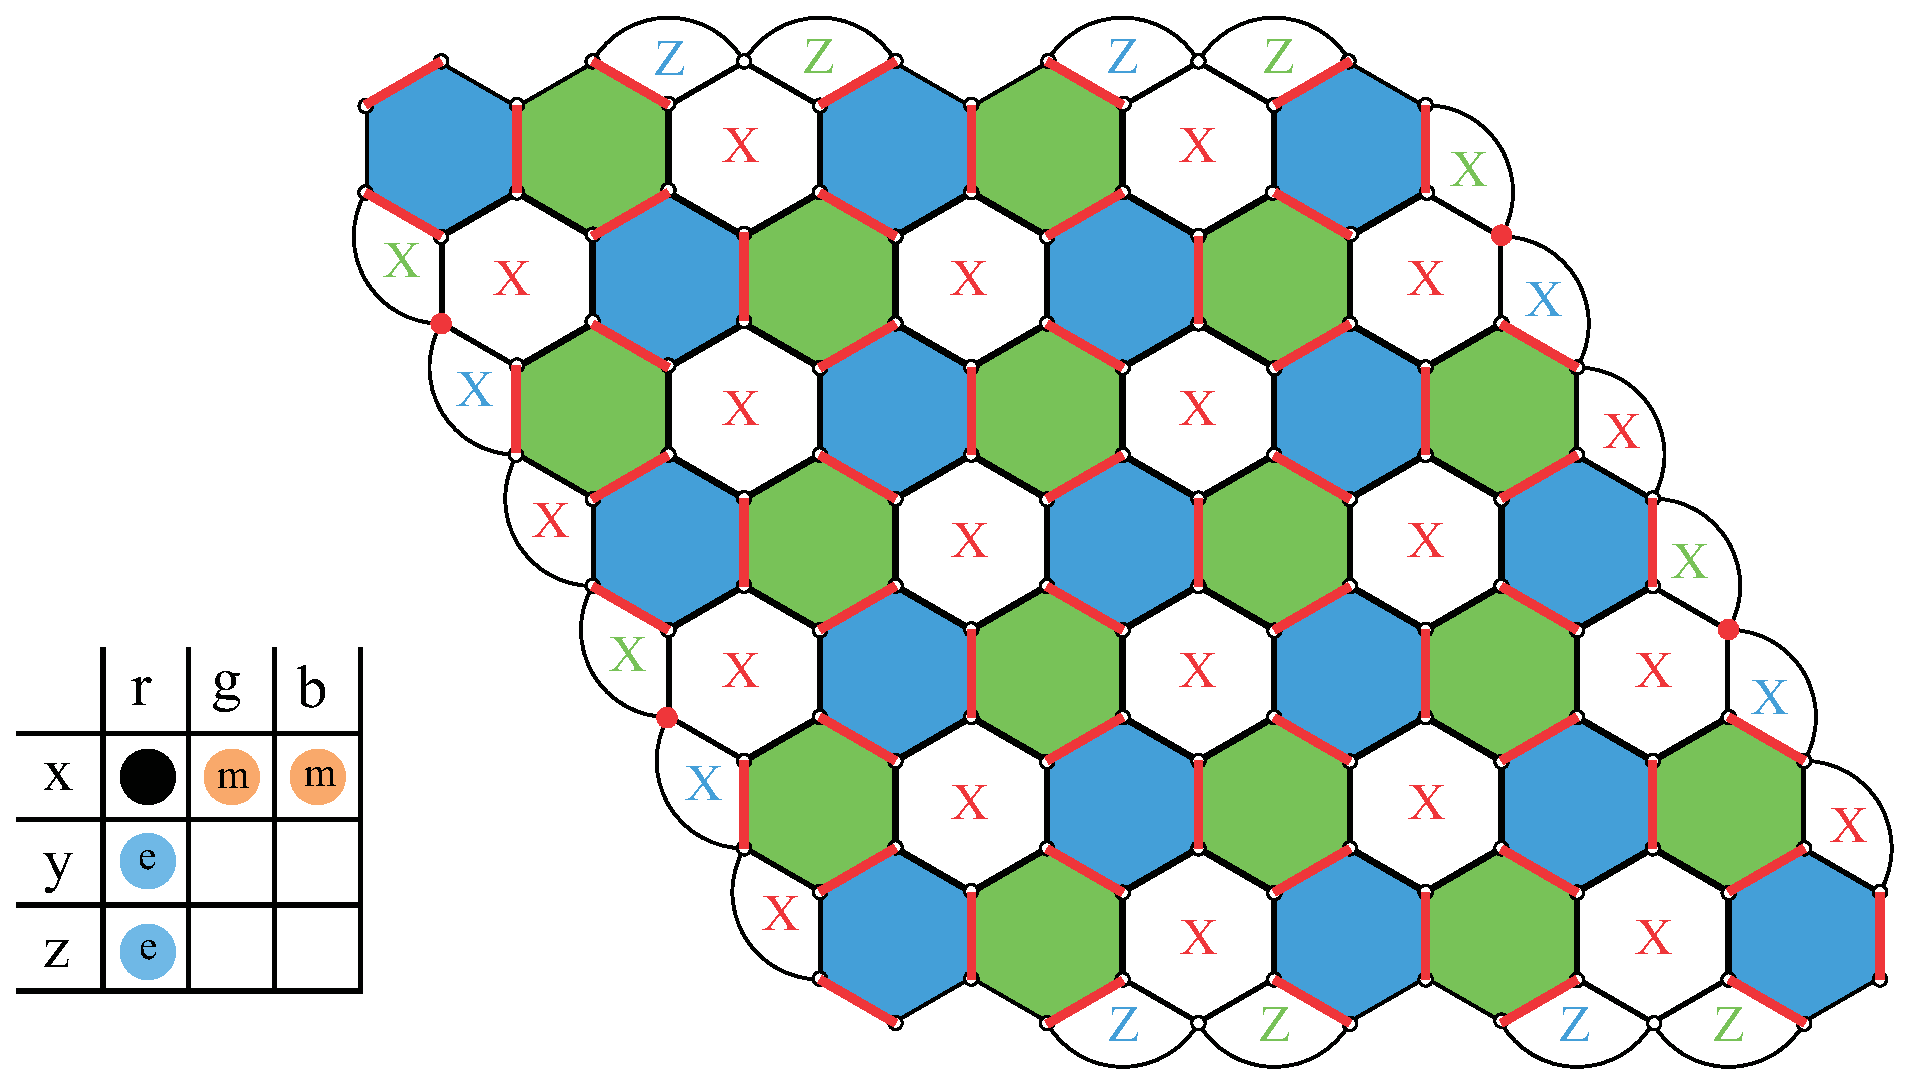
\includegraphics[scale=0.20]{figure2.eps}
    \vspace{25pt}\caption*{(a)}
    \label{}
  \end{minipage}
  \vspace{30pt}\begin{minipage}[h]{0.38\linewidth}
    \scalebox{0.5}[0.5]{
\begin{tikzpicture}[gnuplot]
%% generated with GNUPLOT 5.4p10 (Lua 5.4; terminal rev. Jun 2020, script rev. 118)
%% Sat Dec  9 17:15:40 2023
\path (0.000,0.000) rectangle (12.500,8.750);
\gpcolor{color=gp lt color border}
\gpsetlinetype{gp lt border}
\gpsetdashtype{gp dt solid}
\gpsetlinewidth{1.00}
\draw[gp path] (0.018,0.031)--(0.198,0.031);
\draw[gp path] (12.480,0.031)--(12.300,0.031);
\node[gp node right] at (-0.166,0.031) {$0$};
\draw[gp path] (0.018,0.900)--(0.198,0.900);
\draw[gp path] (12.480,0.900)--(12.300,0.900);
\node[gp node right] at (-0.166,0.900) {$0.1$};
\draw[gp path] (0.018,1.768)--(0.198,1.768);
\draw[gp path] (12.480,1.768)--(12.300,1.768);
\node[gp node right] at (-0.166,1.768) {$0.2$};
\draw[gp path] (0.018,2.637)--(0.198,2.637);
\draw[gp path] (12.480,2.637)--(12.300,2.637);
\node[gp node right] at (-0.166,2.637) {$0.3$};
\draw[gp path] (0.018,3.506)--(0.198,3.506);
\draw[gp path] (12.480,3.506)--(12.300,3.506);
\node[gp node right] at (-0.166,3.506) {$0.4$};
\draw[gp path] (0.018,4.375)--(0.198,4.375);
\draw[gp path] (12.480,4.375)--(12.300,4.375);
\node[gp node right] at (-0.166,4.375) {$0.5$};
\draw[gp path] (0.018,5.243)--(0.198,5.243);
\draw[gp path] (12.480,5.243)--(12.300,5.243);
\node[gp node right] at (-0.166,5.243) {$0.6$};
\draw[gp path] (0.018,6.112)--(0.198,6.112);
\draw[gp path] (12.480,6.112)--(12.300,6.112);
\node[gp node right] at (-0.166,6.112) {$0.7$};
\draw[gp path] (0.018,6.981)--(0.198,6.981);
\draw[gp path] (12.480,6.981)--(12.300,6.981);
\node[gp node right] at (-0.166,6.981) {$0.8$};
\draw[gp path] (0.018,7.849)--(0.198,7.849);
\draw[gp path] (12.480,7.849)--(12.300,7.849);
\node[gp node right] at (-0.166,7.849) {$0.9$};
\draw[gp path] (0.018,8.718)--(0.198,8.718);
\draw[gp path] (12.480,8.718)--(12.300,8.718);
\node[gp node right] at (-0.166,8.718) {$1$};
\draw[gp path] (0.018,0.031)--(0.018,0.211);
\draw[gp path] (0.018,8.718)--(0.018,8.538);
\node[gp node center] at (0.018,-0.277) {$1200$};
\draw[gp path] (1.576,0.031)--(1.576,0.211);
\draw[gp path] (1.576,8.718)--(1.576,8.538);
\node[gp node center] at (1.576,-0.277) {$1250$};
\draw[gp path] (3.134,0.031)--(3.134,0.211);
\draw[gp path] (3.134,8.718)--(3.134,8.538);
\node[gp node center] at (3.134,-0.277) {$1300$};
\draw[gp path] (4.691,0.031)--(4.691,0.211);
\draw[gp path] (4.691,8.718)--(4.691,8.538);
\node[gp node center] at (4.691,-0.277) {$1350$};
\draw[gp path] (6.249,0.031)--(6.249,0.211);
\draw[gp path] (6.249,8.718)--(6.249,8.538);
\node[gp node center] at (6.249,-0.277) {$1400$};
\draw[gp path] (7.807,0.031)--(7.807,0.211);
\draw[gp path] (7.807,8.718)--(7.807,8.538);
\node[gp node center] at (7.807,-0.277) {$1450$};
\draw[gp path] (9.365,0.031)--(9.365,0.211);
\draw[gp path] (9.365,8.718)--(9.365,8.538);
\node[gp node center] at (9.365,-0.277) {$1500$};
\draw[gp path] (10.922,0.031)--(10.922,0.211);
\draw[gp path] (10.922,8.718)--(10.922,8.538);
\node[gp node center] at (10.922,-0.277) {$1550$};
\draw[gp path] (12.480,0.031)--(12.480,0.211);
\draw[gp path] (12.480,8.718)--(12.480,8.538);
\node[gp node center] at (12.480,-0.277) {$1600$};
\draw[gp path] (0.018,8.718)--(0.018,0.031)--(12.480,0.031)--(12.480,8.718)--cycle;
\node[gp node center,rotate=-270,font={\fontsize{17.0pt}{20.4pt}\selectfont}] at (-1.286,4.374) {光強度比P(r)/P(0)};
\node[gp node center,font={\fontsize{17.0pt}{20.4pt}\selectfont}] at (6.249,-1.046) {距離$\ /\ \mathrm{\upmu m}$};
\gpcolor{rgb color={0.000,0.000,0.000}}
\draw[gp path] (0.018,0.406)--(0.064,0.436)--(0.110,0.401)--(0.156,0.380)--(0.202,0.397)%
  --(0.248,0.401)--(0.294,0.432)--(0.340,0.414)--(0.386,0.423)--(0.431,0.401)--(0.477,0.423)%
  --(0.523,0.449)--(0.569,0.410)--(0.615,0.397)--(0.661,0.406)--(0.707,0.427)--(0.753,0.419)%
  --(0.799,0.493)--(0.845,0.454)--(0.891,0.419)--(0.937,0.419)--(0.983,0.397)--(1.029,0.432)%
  --(1.075,0.393)--(1.121,0.410)--(1.167,0.393)--(1.213,0.475)--(1.259,0.401)--(1.305,0.419)%
  --(1.351,0.436)--(1.397,0.427)--(1.443,0.445)--(1.489,0.380)--(1.535,0.441)--(1.581,0.397)%
  --(1.627,0.427)--(1.673,0.471)--(1.719,0.423)--(1.765,0.427)--(1.811,0.427)--(1.857,0.441)%
  --(1.903,0.380)--(1.949,0.419)--(1.995,0.436)--(2.041,0.397)--(2.087,0.445)--(2.133,0.441)%
  --(2.179,0.432)--(2.225,0.462)--(2.271,0.406)--(2.317,0.445)--(2.363,0.493)--(2.409,0.445)%
  --(2.455,0.436)--(2.501,0.454)--(2.547,0.488)--(2.593,0.458)--(2.639,0.436)--(2.685,0.432)%
  --(2.731,0.406)--(2.777,0.401)--(2.823,0.484)--(2.869,0.401)--(2.915,0.441)--(2.961,0.419)%
  --(3.007,0.471)--(3.053,0.497)--(3.099,0.436)--(3.145,0.475)--(3.191,0.432)--(3.237,0.471)%
  --(3.283,0.502)--(3.329,0.484)--(3.375,0.454)--(3.420,0.454)--(3.466,0.471)--(3.512,0.532)%
  --(3.558,0.493)--(3.604,0.532)--(3.650,0.532)--(3.696,0.523)--(3.742,0.515)--(3.788,0.571)%
  --(3.834,0.637)--(3.880,0.689)--(3.926,0.772)--(3.972,0.837)--(4.018,0.955)--(4.064,1.164)%
  --(4.110,1.499)--(4.156,1.874)--(4.202,2.662)--(4.248,3.303)--(4.294,3.582)--(4.340,3.978)%
  --(4.386,4.449)--(4.432,5.276)--(4.478,5.742)--(4.524,6.187)--(4.570,6.409)--(4.616,7.028)%
  --(4.662,7.259)--(4.708,7.320)--(4.754,7.585)--(4.800,7.720)--(4.846,7.564)--(4.892,7.812)%
  --(4.938,7.829)--(4.984,8.012)--(5.030,7.973)--(5.076,8.104)--(5.122,8.165)--(5.168,8.043)%
  --(5.214,7.921)--(5.260,8.252)--(5.306,7.951)--(5.352,8.069)--(5.398,8.112)--(5.444,8.282)%
  --(5.490,7.855)--(5.536,8.291)--(5.582,8.313)--(5.628,8.261)--(5.674,8.078)--(5.720,8.082)%
  --(5.766,8.073)--(5.812,8.208)--(5.858,8.173)--(5.904,8.396)--(5.950,8.221)--(5.996,8.265)%
  --(6.042,8.326)--(6.088,8.165)--(6.134,8.509)--(6.180,8.487)--(6.226,8.579)--(6.272,8.400)%
  --(6.318,8.322)--(6.364,8.304)--(6.410,8.413)--(6.455,8.252)--(6.501,8.230)--(6.547,8.356)%
  --(6.593,8.483)--(6.639,8.452)--(6.685,8.570)--(6.731,8.718)--(6.777,8.635)--(6.823,8.461)%
  --(6.869,8.378)--(6.915,8.444)--(6.961,8.513)--(7.007,8.509)--(7.053,8.396)--(7.099,8.457)%
  --(7.145,8.487)--(7.191,8.535)--(7.237,8.692)--(7.283,8.600)--(7.329,8.574)--(7.375,8.317)%
  --(7.421,8.430)--(7.467,8.500)--(7.513,8.518)--(7.559,8.352)--(7.605,8.644)--(7.651,8.282)%
  --(7.697,8.439)--(7.743,8.535)--(7.789,8.335)--(7.835,8.452)--(7.881,8.304)--(7.927,8.200)%
  --(7.973,8.374)--(8.019,8.374)--(8.065,8.343)--(8.111,8.239)--(8.157,8.365)--(8.203,8.261)%
  --(8.249,8.191)--(8.295,8.226)--(8.341,8.056)--(8.387,8.108)--(8.433,8.461)--(8.479,7.916)%
  --(8.525,8.178)--(8.571,8.073)--(8.617,8.017)--(8.663,8.204)--(8.709,8.282)--(8.755,8.160)%
  --(8.801,7.969)--(8.847,8.348)--(8.893,8.156)--(8.939,8.243)--(8.985,8.086)--(9.031,8.034)%
  --(9.077,8.030)--(9.123,7.947)--(9.169,7.825)--(9.215,8.173)--(9.261,7.908)--(9.307,7.829)%
  --(9.353,7.629)--(9.399,7.276)--(9.445,7.324)--(9.490,7.102)--(9.536,6.901)--(9.582,6.592)%
  --(9.628,6.514)--(9.674,5.773)--(9.720,5.451)--(9.766,4.797)--(9.812,3.616)--(9.858,2.553)%
  --(9.904,2.031)--(9.950,1.608)--(9.996,1.373)--(10.042,1.029)--(10.088,0.981)--(10.134,0.824)%
  --(10.180,0.828)--(10.226,0.671)--(10.272,0.610)--(10.318,0.571)--(10.364,0.502)--(10.410,0.528)%
  --(10.456,0.528)--(10.502,0.506)--(10.548,0.502)--(10.594,0.497)--(10.640,0.445)--(10.686,0.506)%
  --(10.732,0.458)--(10.778,0.427)--(10.824,0.441)--(10.870,0.454)--(10.916,0.475)--(10.962,0.510)%
  --(11.008,0.484)--(11.054,0.423)--(11.100,0.510)--(11.146,0.493)--(11.192,0.519)--(11.238,0.449)%
  --(11.284,0.406)--(11.330,0.449)--(11.376,0.427)--(11.422,0.502)--(11.468,0.436)--(11.514,0.406)%
  --(11.560,0.441)--(11.606,0.423)--(11.652,0.436)--(11.698,0.449)--(11.744,0.471)--(11.790,0.471)%
  --(11.836,0.445)--(11.882,0.423)--(11.928,0.427)--(11.974,0.423)--(12.020,0.427)--(12.066,0.445)%
  --(12.112,0.380)--(12.158,0.441)--(12.204,0.384)--(12.250,0.441)--(12.296,0.414)--(12.342,0.432)%
  --(12.388,0.371)--(12.434,0.419)--(12.480,0.458);
\gpsetpointsize{1.20}
\gp3point{gp mark 7}{}{(0.064,0.436)}
\gp3point{gp mark 7}{}{(0.110,0.401)}
\gp3point{gp mark 7}{}{(0.156,0.380)}
\gp3point{gp mark 7}{}{(0.202,0.397)}
\gp3point{gp mark 7}{}{(0.248,0.401)}
\gp3point{gp mark 7}{}{(0.294,0.432)}
\gp3point{gp mark 7}{}{(0.340,0.414)}
\gp3point{gp mark 7}{}{(0.386,0.423)}
\gp3point{gp mark 7}{}{(0.431,0.401)}
\gp3point{gp mark 7}{}{(0.477,0.423)}
\gp3point{gp mark 7}{}{(0.523,0.449)}
\gp3point{gp mark 7}{}{(0.569,0.410)}
\gp3point{gp mark 7}{}{(0.615,0.397)}
\gp3point{gp mark 7}{}{(0.661,0.406)}
\gp3point{gp mark 7}{}{(0.707,0.427)}
\gp3point{gp mark 7}{}{(0.753,0.419)}
\gp3point{gp mark 7}{}{(0.799,0.493)}
\gp3point{gp mark 7}{}{(0.845,0.454)}
\gp3point{gp mark 7}{}{(0.891,0.419)}
\gp3point{gp mark 7}{}{(0.937,0.419)}
\gp3point{gp mark 7}{}{(0.983,0.397)}
\gp3point{gp mark 7}{}{(1.029,0.432)}
\gp3point{gp mark 7}{}{(1.075,0.393)}
\gp3point{gp mark 7}{}{(1.121,0.410)}
\gp3point{gp mark 7}{}{(1.167,0.393)}
\gp3point{gp mark 7}{}{(1.213,0.475)}
\gp3point{gp mark 7}{}{(1.259,0.401)}
\gp3point{gp mark 7}{}{(1.305,0.419)}
\gp3point{gp mark 7}{}{(1.351,0.436)}
\gp3point{gp mark 7}{}{(1.397,0.427)}
\gp3point{gp mark 7}{}{(1.443,0.445)}
\gp3point{gp mark 7}{}{(1.489,0.380)}
\gp3point{gp mark 7}{}{(1.535,0.441)}
\gp3point{gp mark 7}{}{(1.581,0.397)}
\gp3point{gp mark 7}{}{(1.627,0.427)}
\gp3point{gp mark 7}{}{(1.673,0.471)}
\gp3point{gp mark 7}{}{(1.719,0.423)}
\gp3point{gp mark 7}{}{(1.765,0.427)}
\gp3point{gp mark 7}{}{(1.811,0.427)}
\gp3point{gp mark 7}{}{(1.857,0.441)}
\gp3point{gp mark 7}{}{(1.903,0.380)}
\gp3point{gp mark 7}{}{(1.949,0.419)}
\gp3point{gp mark 7}{}{(1.995,0.436)}
\gp3point{gp mark 7}{}{(2.041,0.397)}
\gp3point{gp mark 7}{}{(2.087,0.445)}
\gp3point{gp mark 7}{}{(2.133,0.441)}
\gp3point{gp mark 7}{}{(2.179,0.432)}
\gp3point{gp mark 7}{}{(2.225,0.462)}
\gp3point{gp mark 7}{}{(2.271,0.406)}
\gp3point{gp mark 7}{}{(2.317,0.445)}
\gp3point{gp mark 7}{}{(2.363,0.493)}
\gp3point{gp mark 7}{}{(2.409,0.445)}
\gp3point{gp mark 7}{}{(2.455,0.436)}
\gp3point{gp mark 7}{}{(2.501,0.454)}
\gp3point{gp mark 7}{}{(2.547,0.488)}
\gp3point{gp mark 7}{}{(2.593,0.458)}
\gp3point{gp mark 7}{}{(2.639,0.436)}
\gp3point{gp mark 7}{}{(2.685,0.432)}
\gp3point{gp mark 7}{}{(2.731,0.406)}
\gp3point{gp mark 7}{}{(2.777,0.401)}
\gp3point{gp mark 7}{}{(2.823,0.484)}
\gp3point{gp mark 7}{}{(2.869,0.401)}
\gp3point{gp mark 7}{}{(2.915,0.441)}
\gp3point{gp mark 7}{}{(2.961,0.419)}
\gp3point{gp mark 7}{}{(3.007,0.471)}
\gp3point{gp mark 7}{}{(3.053,0.497)}
\gp3point{gp mark 7}{}{(3.099,0.436)}
\gp3point{gp mark 7}{}{(3.145,0.475)}
\gp3point{gp mark 7}{}{(3.191,0.432)}
\gp3point{gp mark 7}{}{(3.237,0.471)}
\gp3point{gp mark 7}{}{(3.283,0.502)}
\gp3point{gp mark 7}{}{(3.329,0.484)}
\gp3point{gp mark 7}{}{(3.375,0.454)}
\gp3point{gp mark 7}{}{(3.420,0.454)}
\gp3point{gp mark 7}{}{(3.466,0.471)}
\gp3point{gp mark 7}{}{(3.512,0.532)}
\gp3point{gp mark 7}{}{(3.558,0.493)}
\gp3point{gp mark 7}{}{(3.604,0.532)}
\gp3point{gp mark 7}{}{(3.650,0.532)}
\gp3point{gp mark 7}{}{(3.696,0.523)}
\gp3point{gp mark 7}{}{(3.742,0.515)}
\gp3point{gp mark 7}{}{(3.788,0.571)}
\gp3point{gp mark 7}{}{(3.834,0.637)}
\gp3point{gp mark 7}{}{(3.880,0.689)}
\gp3point{gp mark 7}{}{(3.926,0.772)}
\gp3point{gp mark 7}{}{(3.972,0.837)}
\gp3point{gp mark 7}{}{(4.018,0.955)}
\gp3point{gp mark 7}{}{(4.064,1.164)}
\gp3point{gp mark 7}{}{(4.110,1.499)}
\gp3point{gp mark 7}{}{(4.156,1.874)}
\gp3point{gp mark 7}{}{(4.202,2.662)}
\gp3point{gp mark 7}{}{(4.248,3.303)}
\gp3point{gp mark 7}{}{(4.294,3.582)}
\gp3point{gp mark 7}{}{(4.340,3.978)}
\gp3point{gp mark 7}{}{(4.386,4.449)}
\gp3point{gp mark 7}{}{(4.432,5.276)}
\gp3point{gp mark 7}{}{(4.478,5.742)}
\gp3point{gp mark 7}{}{(4.524,6.187)}
\gp3point{gp mark 7}{}{(4.570,6.409)}
\gp3point{gp mark 7}{}{(4.616,7.028)}
\gp3point{gp mark 7}{}{(4.662,7.259)}
\gp3point{gp mark 7}{}{(4.708,7.320)}
\gp3point{gp mark 7}{}{(4.754,7.585)}
\gp3point{gp mark 7}{}{(4.800,7.720)}
\gp3point{gp mark 7}{}{(4.846,7.564)}
\gp3point{gp mark 7}{}{(4.892,7.812)}
\gp3point{gp mark 7}{}{(4.938,7.829)}
\gp3point{gp mark 7}{}{(4.984,8.012)}
\gp3point{gp mark 7}{}{(5.030,7.973)}
\gp3point{gp mark 7}{}{(5.076,8.104)}
\gp3point{gp mark 7}{}{(5.122,8.165)}
\gp3point{gp mark 7}{}{(5.168,8.043)}
\gp3point{gp mark 7}{}{(5.214,7.921)}
\gp3point{gp mark 7}{}{(5.260,8.252)}
\gp3point{gp mark 7}{}{(5.306,7.951)}
\gp3point{gp mark 7}{}{(5.352,8.069)}
\gp3point{gp mark 7}{}{(5.398,8.112)}
\gp3point{gp mark 7}{}{(5.444,8.282)}
\gp3point{gp mark 7}{}{(5.490,7.855)}
\gp3point{gp mark 7}{}{(5.536,8.291)}
\gp3point{gp mark 7}{}{(5.582,8.313)}
\gp3point{gp mark 7}{}{(5.628,8.261)}
\gp3point{gp mark 7}{}{(5.674,8.078)}
\gp3point{gp mark 7}{}{(5.720,8.082)}
\gp3point{gp mark 7}{}{(5.766,8.073)}
\gp3point{gp mark 7}{}{(5.812,8.208)}
\gp3point{gp mark 7}{}{(5.858,8.173)}
\gp3point{gp mark 7}{}{(5.904,8.396)}
\gp3point{gp mark 7}{}{(5.950,8.221)}
\gp3point{gp mark 7}{}{(5.996,8.265)}
\gp3point{gp mark 7}{}{(6.042,8.326)}
\gp3point{gp mark 7}{}{(6.088,8.165)}
\gp3point{gp mark 7}{}{(6.134,8.509)}
\gp3point{gp mark 7}{}{(6.180,8.487)}
\gp3point{gp mark 7}{}{(6.226,8.579)}
\gp3point{gp mark 7}{}{(6.272,8.400)}
\gp3point{gp mark 7}{}{(6.318,8.322)}
\gp3point{gp mark 7}{}{(6.364,8.304)}
\gp3point{gp mark 7}{}{(6.410,8.413)}
\gp3point{gp mark 7}{}{(6.455,8.252)}
\gp3point{gp mark 7}{}{(6.501,8.230)}
\gp3point{gp mark 7}{}{(6.547,8.356)}
\gp3point{gp mark 7}{}{(6.593,8.483)}
\gp3point{gp mark 7}{}{(6.639,8.452)}
\gp3point{gp mark 7}{}{(6.685,8.570)}
\gp3point{gp mark 7}{}{(6.731,8.718)}
\gp3point{gp mark 7}{}{(6.777,8.635)}
\gp3point{gp mark 7}{}{(6.823,8.461)}
\gp3point{gp mark 7}{}{(6.869,8.378)}
\gp3point{gp mark 7}{}{(6.915,8.444)}
\gp3point{gp mark 7}{}{(6.961,8.513)}
\gp3point{gp mark 7}{}{(7.007,8.509)}
\gp3point{gp mark 7}{}{(7.053,8.396)}
\gp3point{gp mark 7}{}{(7.099,8.457)}
\gp3point{gp mark 7}{}{(7.145,8.487)}
\gp3point{gp mark 7}{}{(7.191,8.535)}
\gp3point{gp mark 7}{}{(7.237,8.692)}
\gp3point{gp mark 7}{}{(7.283,8.600)}
\gp3point{gp mark 7}{}{(7.329,8.574)}
\gp3point{gp mark 7}{}{(7.375,8.317)}
\gp3point{gp mark 7}{}{(7.421,8.430)}
\gp3point{gp mark 7}{}{(7.467,8.500)}
\gp3point{gp mark 7}{}{(7.513,8.518)}
\gp3point{gp mark 7}{}{(7.559,8.352)}
\gp3point{gp mark 7}{}{(7.605,8.644)}
\gp3point{gp mark 7}{}{(7.651,8.282)}
\gp3point{gp mark 7}{}{(7.697,8.439)}
\gp3point{gp mark 7}{}{(7.743,8.535)}
\gp3point{gp mark 7}{}{(7.789,8.335)}
\gp3point{gp mark 7}{}{(7.835,8.452)}
\gp3point{gp mark 7}{}{(7.881,8.304)}
\gp3point{gp mark 7}{}{(7.927,8.200)}
\gp3point{gp mark 7}{}{(7.973,8.374)}
\gp3point{gp mark 7}{}{(8.019,8.374)}
\gp3point{gp mark 7}{}{(8.065,8.343)}
\gp3point{gp mark 7}{}{(8.111,8.239)}
\gp3point{gp mark 7}{}{(8.157,8.365)}
\gp3point{gp mark 7}{}{(8.203,8.261)}
\gp3point{gp mark 7}{}{(8.249,8.191)}
\gp3point{gp mark 7}{}{(8.295,8.226)}
\gp3point{gp mark 7}{}{(8.341,8.056)}
\gp3point{gp mark 7}{}{(8.387,8.108)}
\gp3point{gp mark 7}{}{(8.433,8.461)}
\gp3point{gp mark 7}{}{(8.479,7.916)}
\gp3point{gp mark 7}{}{(8.525,8.178)}
\gp3point{gp mark 7}{}{(8.571,8.073)}
\gp3point{gp mark 7}{}{(8.617,8.017)}
\gp3point{gp mark 7}{}{(8.663,8.204)}
\gp3point{gp mark 7}{}{(8.709,8.282)}
\gp3point{gp mark 7}{}{(8.755,8.160)}
\gp3point{gp mark 7}{}{(8.801,7.969)}
\gp3point{gp mark 7}{}{(8.847,8.348)}
\gp3point{gp mark 7}{}{(8.893,8.156)}
\gp3point{gp mark 7}{}{(8.939,8.243)}
\gp3point{gp mark 7}{}{(8.985,8.086)}
\gp3point{gp mark 7}{}{(9.031,8.034)}
\gp3point{gp mark 7}{}{(9.077,8.030)}
\gp3point{gp mark 7}{}{(9.123,7.947)}
\gp3point{gp mark 7}{}{(9.169,7.825)}
\gp3point{gp mark 7}{}{(9.215,8.173)}
\gp3point{gp mark 7}{}{(9.261,7.908)}
\gp3point{gp mark 7}{}{(9.307,7.829)}
\gp3point{gp mark 7}{}{(9.353,7.629)}
\gp3point{gp mark 7}{}{(9.399,7.276)}
\gp3point{gp mark 7}{}{(9.445,7.324)}
\gp3point{gp mark 7}{}{(9.490,7.102)}
\gp3point{gp mark 7}{}{(9.536,6.901)}
\gp3point{gp mark 7}{}{(9.582,6.592)}
\gp3point{gp mark 7}{}{(9.628,6.514)}
\gp3point{gp mark 7}{}{(9.674,5.773)}
\gp3point{gp mark 7}{}{(9.720,5.451)}
\gp3point{gp mark 7}{}{(9.766,4.797)}
\gp3point{gp mark 7}{}{(9.812,3.616)}
\gp3point{gp mark 7}{}{(9.858,2.553)}
\gp3point{gp mark 7}{}{(9.904,2.031)}
\gp3point{gp mark 7}{}{(9.950,1.608)}
\gp3point{gp mark 7}{}{(9.996,1.373)}
\gp3point{gp mark 7}{}{(10.042,1.029)}
\gp3point{gp mark 7}{}{(10.088,0.981)}
\gp3point{gp mark 7}{}{(10.134,0.824)}
\gp3point{gp mark 7}{}{(10.180,0.828)}
\gp3point{gp mark 7}{}{(10.226,0.671)}
\gp3point{gp mark 7}{}{(10.272,0.610)}
\gp3point{gp mark 7}{}{(10.318,0.571)}
\gp3point{gp mark 7}{}{(10.364,0.502)}
\gp3point{gp mark 7}{}{(10.410,0.528)}
\gp3point{gp mark 7}{}{(10.456,0.528)}
\gp3point{gp mark 7}{}{(10.502,0.506)}
\gp3point{gp mark 7}{}{(10.548,0.502)}
\gp3point{gp mark 7}{}{(10.594,0.497)}
\gp3point{gp mark 7}{}{(10.640,0.445)}
\gp3point{gp mark 7}{}{(10.686,0.506)}
\gp3point{gp mark 7}{}{(10.732,0.458)}
\gp3point{gp mark 7}{}{(10.778,0.427)}
\gp3point{gp mark 7}{}{(10.824,0.441)}
\gp3point{gp mark 7}{}{(10.870,0.454)}
\gp3point{gp mark 7}{}{(10.916,0.475)}
\gp3point{gp mark 7}{}{(10.962,0.510)}
\gp3point{gp mark 7}{}{(11.008,0.484)}
\gp3point{gp mark 7}{}{(11.054,0.423)}
\gp3point{gp mark 7}{}{(11.100,0.510)}
\gp3point{gp mark 7}{}{(11.146,0.493)}
\gp3point{gp mark 7}{}{(11.192,0.519)}
\gp3point{gp mark 7}{}{(11.238,0.449)}
\gp3point{gp mark 7}{}{(11.284,0.406)}
\gp3point{gp mark 7}{}{(11.330,0.449)}
\gp3point{gp mark 7}{}{(11.376,0.427)}
\gp3point{gp mark 7}{}{(11.422,0.502)}
\gp3point{gp mark 7}{}{(11.468,0.436)}
\gp3point{gp mark 7}{}{(11.514,0.406)}
\gp3point{gp mark 7}{}{(11.560,0.441)}
\gp3point{gp mark 7}{}{(11.606,0.423)}
\gp3point{gp mark 7}{}{(11.652,0.436)}
\gp3point{gp mark 7}{}{(11.698,0.449)}
\gp3point{gp mark 7}{}{(11.744,0.471)}
\gp3point{gp mark 7}{}{(11.790,0.471)}
\gp3point{gp mark 7}{}{(11.836,0.445)}
\gp3point{gp mark 7}{}{(11.882,0.423)}
\gp3point{gp mark 7}{}{(11.928,0.427)}
\gp3point{gp mark 7}{}{(11.974,0.423)}
\gp3point{gp mark 7}{}{(12.020,0.427)}
\gp3point{gp mark 7}{}{(12.066,0.445)}
\gp3point{gp mark 7}{}{(12.112,0.380)}
\gp3point{gp mark 7}{}{(12.158,0.441)}
\gp3point{gp mark 7}{}{(12.204,0.384)}
\gp3point{gp mark 7}{}{(12.250,0.441)}
\gp3point{gp mark 7}{}{(12.296,0.414)}
\gp3point{gp mark 7}{}{(12.342,0.432)}
\gp3point{gp mark 7}{}{(12.388,0.371)}
\gp3point{gp mark 7}{}{(12.434,0.419)}
\gp3point{gp mark 7}{}{(12.480,0.458)}
\gpcolor{color=gp lt color border}
\draw[gp path] (0.018,8.718)--(0.018,0.031)--(12.480,0.031)--(12.480,8.718)--cycle;
%% coordinates of the plot area
\gpdefrectangularnode{gp plot 1}{\pgfpoint{0.018cm}{0.031cm}}{\pgfpoint{12.480cm}{8.718cm}}%% gnuplot variables
\end{tikzpicture}
}

    \vspace{-30pt}\caption*{(b)}
    \label{}
  \end{minipage}
  \vspace{-30pt}\caption{SI型について、(a)撮影したNFPの写真\ (b)光強度分布}
  \label{SI}
\end{figure}
図\ref{GI}から、GI型のコア径は$200\ \mathrm{\upmu m}$、図\ref{SI}から、SI型のコア径は$50\ \mathrm{\upmu m}$であることがわかる。\\
\\
{\large \bfseries 2.4 光ファイバの伝送帯域特性}\\
\begin{table}[h]
  \newcolumntype{I}{!{\vrule width 1.5pt}}
  \newcolumntype{i}{!{\vrule width 0.8pt}}
  \arrayrulewidth=0.8pt
  \renewcommand{\arraystretch}{1.5}
  \newcommand{\bhline}[1]{\noalign{\hrule height #1}}
  \centering
  \caption{光ファイバの出射光強度}
  \label{lengthefficiency}
  \begin{tabular}{IcicccI}
    \bhline{1.5pt}
    ファイバ被覆の色&ファイバ長\ /\ m&FWHM\ /\ ps&実測した伝送帯域\ /\ MHz\\
    \bhline{0.5pt}
    白色&100&769&956\\
    橙色&100&265&1100\\
    水色&100&129&2640\\
    \bhline{1.5pt}
  \end{tabular}
\end{table}
表\ref{lengthefficiency}と補足データからファイバ長とFWHMの関係を図\ref{fiberlength-FWHM}に、ファイバ長と伝送帯域の関係を図\ref{fiberlength-Hz}に示す。
\begin{figure}[h]
  \centering
  \scalebox{0.45}[0.45]{
\begin{tikzpicture}[gnuplot]
%% generated with GNUPLOT 5.4p10 (Lua 5.4; terminal rev. Jun 2020, script rev. 118)
%% Sun Nov 19 19:22:08 2023
\path (0.000,0.000) rectangle (12.500,8.750);
\gpcolor{color=gp lt color border}
\gpsetlinetype{gp lt border}
\gpsetdashtype{gp dt solid}
\gpsetlinewidth{1.00}
\draw[gp path] (0.018,0.031)--(0.198,0.031);
\draw[gp path] (12.480,0.031)--(12.300,0.031);
\node[gp node right] at (-0.166,0.031) {$-200$};
\draw[gp path] (0.018,1.768)--(0.198,1.768);
\draw[gp path] (12.480,1.768)--(12.300,1.768);
\node[gp node right] at (-0.166,1.768) {$-150$};
\draw[gp path] (0.018,3.506)--(0.198,3.506);
\draw[gp path] (12.480,3.506)--(12.300,3.506);
\node[gp node right] at (-0.166,3.506) {$-100$};
\draw[gp path] (0.018,5.243)--(0.198,5.243);
\draw[gp path] (12.480,5.243)--(12.300,5.243);
\node[gp node right] at (-0.166,5.243) {$-50$};
\draw[gp path] (0.018,6.981)--(0.198,6.981);
\draw[gp path] (12.480,6.981)--(12.300,6.981);
\node[gp node right] at (-0.166,6.981) {$0$};
\draw[gp path] (0.018,8.718)--(0.198,8.718);
\draw[gp path] (12.480,8.718)--(12.300,8.718);
\node[gp node right] at (-0.166,8.718) {$50$};
\draw[gp path] (0.018,0.031)--(0.018,0.211);
\draw[gp path] (0.018,8.718)--(0.018,8.538);
\node[gp node center] at (0.018,-0.277) {$0$};
\draw[gp path] (1.330,0.031)--(1.330,0.211);
\draw[gp path] (1.330,8.718)--(1.330,8.538);
\node[gp node center] at (1.330,-0.277) {$2$};
\draw[gp path] (2.642,0.031)--(2.642,0.211);
\draw[gp path] (2.642,8.718)--(2.642,8.538);
\node[gp node center] at (2.642,-0.277) {$4$};
\draw[gp path] (3.953,0.031)--(3.953,0.211);
\draw[gp path] (3.953,8.718)--(3.953,8.538);
\node[gp node center] at (3.953,-0.277) {$6$};
\draw[gp path] (5.265,0.031)--(5.265,0.211);
\draw[gp path] (5.265,8.718)--(5.265,8.538);
\node[gp node center] at (5.265,-0.277) {$8$};
\draw[gp path] (6.577,0.031)--(6.577,0.211);
\draw[gp path] (6.577,8.718)--(6.577,8.538);
\node[gp node center] at (6.577,-0.277) {$10$};
\draw[gp path] (7.889,0.031)--(7.889,0.211);
\draw[gp path] (7.889,8.718)--(7.889,8.538);
\node[gp node center] at (7.889,-0.277) {$12$};
\draw[gp path] (9.201,0.031)--(9.201,0.211);
\draw[gp path] (9.201,8.718)--(9.201,8.538);
\node[gp node center] at (9.201,-0.277) {$14$};
\draw[gp path] (10.512,0.031)--(10.512,0.211);
\draw[gp path] (10.512,8.718)--(10.512,8.538);
\node[gp node center] at (10.512,-0.277) {$16$};
\draw[gp path] (11.824,0.031)--(11.824,0.211);
\draw[gp path] (11.824,8.718)--(11.824,8.538);
\node[gp node center] at (11.824,-0.277) {$18$};
\draw[gp path] (0.018,8.718)--(0.018,0.031)--(12.480,0.031)--(12.480,8.718)--cycle;
\node[gp node center,rotate=-270] at (-1.194,4.374) {角速度$\dot{\theta}\ /\ \mathrm{^\circ\cdot s^{-1}}$};
\node[gp node center] at (6.249,-0.738) {時間$t\ /\  \mathrm{s}$};
\gpcolor{rgb color={0.000,0.000,0.000}}
\draw[gp path] (0.018,5.334)--(0.031,1.979)--(0.044,0.221)--(0.057,1.269)--(0.070,3.077)%
  --(0.084,4.818)--(0.097,6.086)--(0.110,6.877)--(0.123,7.368)--(0.136,7.490)--(0.149,7.350)%
  --(0.162,7.388)--(0.175,7.358)--(0.189,7.465)--(0.202,7.530)--(0.215,7.524)--(0.228,7.397)%
  --(0.241,7.253)--(0.254,7.302)--(0.267,7.036)--(0.280,6.958)--(0.293,6.890)--(0.307,6.901)%
  --(0.320,6.883)--(0.333,6.724)--(0.346,6.712)--(0.359,6.772)--(0.372,6.672)--(0.385,6.589)%
  --(0.398,6.540)--(0.412,6.259)--(0.425,6.400)--(0.438,6.532)--(0.451,6.779)--(0.464,6.823)%
  --(0.477,6.719)--(0.490,6.743)--(0.503,6.614)--(0.516,6.665)--(0.530,6.894)--(0.543,7.058)%
  --(0.556,7.303)--(0.569,7.381)--(0.582,7.366)--(0.595,7.347)--(0.608,7.358)--(0.621,7.334)%
  --(0.635,7.389)--(0.648,7.626)--(0.661,7.636)--(0.674,7.345)--(0.687,7.058)--(0.700,6.984)%
  --(0.713,6.991)--(0.726,7.047)--(0.739,7.165)--(0.753,7.137)--(0.766,7.238)--(0.779,7.368)%
  --(0.792,7.207)--(0.805,7.040)--(0.818,6.897)--(0.831,6.821)--(0.844,6.771)--(0.858,6.689)%
  --(0.871,6.598)--(0.884,6.537)--(0.897,6.570)--(0.910,6.742)--(0.923,6.737)--(0.936,6.579)%
  --(0.949,6.408)--(0.962,6.371)--(0.976,6.420)--(0.989,6.505)--(1.002,6.592)--(1.015,6.638)%
  --(1.028,6.721)--(1.041,6.561)--(1.054,6.549)--(1.067,6.657)--(1.081,6.882)--(1.094,7.031)%
  --(1.107,7.215)--(1.120,7.391)--(1.133,7.392)--(1.146,7.449)--(1.159,7.524)--(1.172,7.400)%
  --(1.185,7.420)--(1.199,7.499)--(1.212,7.285)--(1.225,7.029)--(1.238,6.912)--(1.251,6.880)%
  --(1.264,6.958)--(1.277,6.952)--(1.290,7.015)--(1.304,6.968)--(1.317,6.958)--(1.330,7.011)%
  --(1.343,6.845)--(1.356,6.484)--(1.369,6.463)--(1.382,6.444)--(1.395,6.324)--(1.408,6.235)%
  --(1.422,6.208)--(1.435,6.276)--(1.448,6.292)--(1.461,6.321)--(1.474,6.323)--(1.487,6.355)%
  --(1.500,6.345)--(1.513,6.358)--(1.527,6.449)--(1.540,6.535)--(1.553,6.528)--(1.566,6.526)%
  --(1.579,6.546)--(1.592,6.588)--(1.605,6.756)--(1.618,7.047)--(1.632,6.911)--(1.645,6.672)%
  --(1.658,6.578)--(1.671,7.038)--(1.684,7.272)--(1.697,7.340)--(1.710,7.460)--(1.723,7.319)%
  --(1.736,7.057)--(1.750,7.072)--(1.763,7.056)--(1.776,7.089)--(1.789,7.033)--(1.802,6.825)%
  --(1.815,6.800)--(1.828,6.865)--(1.841,6.901)--(1.855,6.845)--(1.868,6.780)--(1.881,6.801)%
  --(1.894,6.821)--(1.907,6.815)--(1.920,6.827)--(1.933,6.844)--(1.946,6.818)--(1.959,6.736)%
  --(1.973,6.707)--(1.986,6.699)--(1.999,6.670)--(2.012,6.820)--(2.025,6.983)--(2.038,6.939)%
  --(2.051,6.817)--(2.064,6.858)--(2.078,7.056)--(2.091,7.265)--(2.104,7.249)--(2.117,7.270)%
  --(2.130,7.962)--(2.143,8.668)--(2.156,7.928)--(2.169,6.663)--(2.182,6.607)--(2.196,7.185)%
  --(2.209,7.350)--(2.222,7.265)--(2.235,7.214)--(2.248,7.206)--(2.261,7.281)--(2.274,7.396)%
  --(2.287,7.509)--(2.301,7.450)--(2.314,7.489)--(2.327,7.474)--(2.340,7.465)--(2.353,7.565)%
  --(2.366,7.768)--(2.379,7.484)--(2.392,7.064)--(2.405,6.948)--(2.419,7.242)--(2.432,7.422)%
  --(2.445,7.260)--(2.458,6.993)--(2.471,6.852)--(2.484,6.827)--(2.497,6.853)--(2.510,6.848)%
  --(2.524,6.835)--(2.537,6.786)--(2.550,6.702)--(2.563,6.727)--(2.576,6.773)--(2.589,6.861)%
  --(2.602,6.997)--(2.615,6.886)--(2.628,6.750)--(2.642,6.641)--(2.655,6.712)--(2.668,6.755)%
  --(2.681,6.824)--(2.694,6.821)--(2.707,6.823)--(2.720,6.887)--(2.733,7.068)--(2.747,6.928)%
  --(2.760,6.717)--(2.773,6.597)--(2.786,6.450)--(2.799,6.736)--(2.812,7.016)--(2.825,7.287)%
  --(2.838,8.097)--(2.851,8.526)--(2.865,7.998)--(2.878,7.193)--(2.891,6.977)--(2.904,7.041)%
  --(2.917,7.192)--(2.930,7.419)--(2.943,7.751)--(2.956,7.926)--(2.970,7.836)--(2.983,7.591)%
  --(2.996,7.564)--(3.009,7.582)--(3.022,7.364)--(3.035,7.174)--(3.048,7.230)--(3.061,7.325)%
  --(3.074,7.345)--(3.088,7.452)--(3.101,7.664)--(3.114,7.648)--(3.127,7.406)--(3.140,7.121)%
  --(3.153,6.952)--(3.166,6.838)--(3.179,6.823)--(3.193,6.871)--(3.206,6.950)--(3.219,7.003)%
  --(3.232,6.876)--(3.245,6.730)--(3.258,6.628)--(3.271,6.703)--(3.284,6.789)--(3.297,6.838)%
  --(3.311,6.797)--(3.324,6.804)--(3.337,6.841)--(3.350,6.856)--(3.363,6.842)--(3.376,6.881)%
  --(3.389,6.954)--(3.402,6.912)--(3.416,6.838)--(3.429,6.790)--(3.442,6.815)--(3.455,6.844)%
  --(3.468,6.847)--(3.481,6.885)--(3.494,6.984)--(3.507,7.117)--(3.520,7.230)--(3.534,7.344)%
  --(3.547,7.418)--(3.560,7.503)--(3.573,7.608)--(3.586,7.667)--(3.599,7.738)--(3.612,7.880)%
  --(3.625,7.846)--(3.639,7.781)--(3.652,7.890)--(3.665,7.955)--(3.678,7.866)--(3.691,7.756)%
  --(3.704,7.718)--(3.717,7.718)--(3.730,7.685)--(3.743,7.709)--(3.757,7.502)--(3.770,7.141)%
  --(3.783,6.743)--(3.796,6.276)--(3.809,5.820)--(3.822,5.451)--(3.835,5.432)--(3.848,5.696)%
  --(3.862,5.993)--(3.875,6.189)--(3.888,6.314)--(3.901,6.460)--(3.914,6.614)--(3.927,6.761)%
  --(3.940,6.707)--(3.953,6.709)--(3.966,6.703)--(3.980,6.736)--(3.993,6.800)--(4.006,6.996)%
  --(4.019,7.060)--(4.032,7.056)--(4.045,7.054)--(4.058,7.071)--(4.071,7.104)--(4.085,7.041)%
  --(4.098,7.110)--(4.111,7.342)--(4.124,7.608)--(4.137,7.776)--(4.150,7.713)--(4.163,7.544)%
  --(4.176,7.390)--(4.189,7.222)--(4.203,7.031)--(4.216,6.926)--(4.229,6.858)--(4.242,6.935)%
  --(4.255,7.042)--(4.268,7.094)--(4.281,7.158)--(4.294,7.143)--(4.308,7.031)--(4.321,6.950)%
  --(4.334,6.949)--(4.347,6.986)--(4.360,7.025)--(4.373,7.062)--(4.386,7.085)--(4.399,7.090)%
  --(4.412,7.090)--(4.426,7.146)--(4.439,7.216)--(4.452,7.136)--(4.465,6.983)--(4.478,6.934)%
  --(4.491,6.910)--(4.504,7.006)--(4.517,7.114)--(4.531,7.085)--(4.544,6.986)--(4.557,6.935)%
  --(4.570,6.926)--(4.583,6.922)--(4.596,6.968)--(4.609,7.081)--(4.622,7.116)--(4.635,6.998)%
  --(4.649,6.888)--(4.662,6.875)--(4.675,6.922)--(4.688,6.963)--(4.701,6.992)--(4.714,7.023)%
  --(4.727,7.038)--(4.740,7.066)--(4.754,7.098)--(4.767,7.122)--(4.780,7.118)--(4.793,7.147)%
  --(4.806,7.184)--(4.819,7.114)--(4.832,7.028)--(4.845,6.987)--(4.859,6.939)--(4.872,6.940)%
  --(4.885,6.985)--(4.898,6.945)--(4.911,6.882)--(4.924,6.907)--(4.937,6.994)--(4.950,7.103)%
  --(4.963,7.182)--(4.977,7.250)--(4.990,7.288)--(5.003,7.328)--(5.016,7.336)--(5.029,7.355)%
  --(5.042,7.349)--(5.055,7.250)--(5.068,7.183)--(5.082,7.194)--(5.095,7.222)--(5.108,7.205)%
  --(5.121,7.180)--(5.134,7.200)--(5.147,7.221)--(5.160,7.163)--(5.173,7.093)--(5.186,7.060)%
  --(5.200,7.072)--(5.213,7.117)--(5.226,7.159)--(5.239,7.152)--(5.252,7.160)--(5.265,7.187)%
  --(5.278,7.144)--(5.291,7.091)--(5.305,7.083)--(5.318,7.090)--(5.331,7.099)--(5.344,7.114)%
  --(5.357,7.136)--(5.370,7.154)--(5.383,7.180)--(5.396,7.211)--(5.409,7.213)--(5.423,7.208)%
  --(5.436,7.199)--(5.449,7.195)--(5.462,7.199)--(5.475,7.190)--(5.488,7.168)--(5.501,7.170)%
  --(5.514,7.205)--(5.528,7.198)--(5.541,7.153)--(5.554,7.118)--(5.567,7.116)--(5.580,7.122)%
  --(5.593,7.131)--(5.606,7.150)--(5.619,7.118)--(5.632,7.082)--(5.646,7.066)--(5.659,7.070)%
  --(5.672,7.085)--(5.685,7.133)--(5.698,7.174)--(5.711,7.158)--(5.724,7.127)--(5.737,7.109)%
  --(5.751,7.060)--(5.764,6.997)--(5.777,6.963)--(5.790,6.954)--(5.803,6.968)--(5.816,6.971)%
  --(5.829,6.938)--(5.842,6.909)--(5.855,6.895)--(5.869,6.897)--(5.882,6.904)--(5.895,6.900)%
  --(5.908,6.929)--(5.921,6.939)--(5.934,6.942)--(5.947,6.933)--(5.960,6.925)--(5.974,6.917)%
  --(5.987,6.855)--(6.000,6.818)--(6.013,6.836)--(6.026,6.862)--(6.039,6.860)--(6.052,6.894)%
  --(6.065,6.926)--(6.078,6.991)--(6.092,7.122)--(6.105,7.123)--(6.118,7.130)--(6.131,7.184)%
  --(6.144,7.217)--(6.157,7.237)--(6.170,7.235)--(6.183,7.203)--(6.197,7.183)--(6.210,7.215)%
  --(6.223,7.253)--(6.236,7.300)--(6.249,7.306)--(6.262,7.293)--(6.275,7.389)--(6.288,7.399)%
  --(6.301,7.371)--(6.315,7.336)--(6.328,7.209)--(6.341,7.121)--(6.354,7.090)--(6.367,7.013)%
  --(6.380,6.945)--(6.393,6.900)--(6.406,6.843)--(6.420,6.792)--(6.433,6.755)--(6.446,6.730)%
  --(6.459,6.687)--(6.472,6.661)--(6.485,6.579)--(6.498,6.531)--(6.511,6.505)--(6.524,6.579)%
  --(6.538,6.700)--(6.551,6.789)--(6.564,6.734)--(6.577,6.707)--(6.590,6.758)--(6.603,6.774)%
  --(6.616,6.715)--(6.629,6.510)--(6.643,6.638)--(6.656,6.823)--(6.669,7.013)--(6.682,7.183)%
  --(6.695,7.377)--(6.708,7.460)--(6.721,7.512)--(6.734,7.485)--(6.747,7.503)--(6.761,7.517)%
  --(6.774,7.470)--(6.787,7.544)--(6.800,7.382)--(6.813,7.350)--(6.826,7.367)--(6.839,7.291)%
  --(6.852,7.212)--(6.866,7.208)--(6.879,7.107)--(6.892,7.001)--(6.905,6.922)--(6.918,6.780)%
  --(6.931,6.728)--(6.944,6.610)--(6.957,6.529)--(6.970,6.480)--(6.984,6.460)--(6.997,6.448)%
  --(7.010,6.442)--(7.023,6.449)--(7.036,6.477)--(7.049,6.509)--(7.062,6.523)--(7.075,6.592)%
  --(7.089,6.624)--(7.102,6.667)--(7.115,6.597)--(7.128,6.762)--(7.141,6.725)--(7.154,6.715)%
  --(7.167,6.810)--(7.180,6.813)--(7.193,6.799)--(7.207,6.860)--(7.220,6.925)--(7.233,6.926)%
  --(7.246,7.058)--(7.259,7.272)--(7.272,7.429)--(7.285,7.551)--(7.298,7.542)--(7.312,7.538)%
  --(7.325,7.566)--(7.338,7.598)--(7.351,7.609)--(7.364,7.556)--(7.377,7.535)--(7.390,7.578)%
  --(7.403,7.521)--(7.416,7.450)--(7.430,7.470)--(7.443,7.351)--(7.456,7.246)--(7.469,7.150)%
  --(7.482,7.086)--(7.495,6.973)--(7.508,6.830)--(7.521,6.728)--(7.535,6.558)--(7.548,6.479)%
  --(7.561,6.446)--(7.574,6.409)--(7.587,6.368)--(7.600,6.320)--(7.613,6.270)--(7.626,6.211)%
  --(7.639,6.100)--(7.653,6.092)--(7.666,6.090)--(7.679,5.917)--(7.692,5.772)--(7.705,5.689)%
  --(7.718,5.645)--(7.731,5.770)--(7.744,5.872)--(7.758,6.168)--(7.771,6.512)--(7.784,6.684)%
  --(7.797,6.770)--(7.810,6.918)--(7.823,7.053)--(7.836,7.081)--(7.849,7.292)--(7.863,7.608)%
  --(7.876,7.440)--(7.889,7.244)--(7.902,7.246)--(7.915,7.377)--(7.928,7.504)--(7.941,7.491)%
  --(7.954,7.448)--(7.967,7.388)--(7.981,7.409)--(7.994,7.351)--(8.007,7.289)--(8.020,7.191)%
  --(8.033,7.169)--(8.046,7.127)--(8.059,7.050)--(8.072,7.004)--(8.086,6.906)--(8.099,6.687)%
  --(8.112,6.647)--(8.125,6.587)--(8.138,6.561)--(8.151,6.531)--(8.164,6.598)--(8.177,6.669)%
  --(8.190,6.576)--(8.204,6.431)--(8.217,6.263)--(8.230,6.373)--(8.243,6.704)--(8.256,6.891)%
  --(8.269,6.911)--(8.282,6.883)--(8.295,6.807)--(8.309,6.732)--(8.322,6.690)--(8.335,6.707)%
  --(8.348,6.751)--(8.361,6.811)--(8.374,6.910)--(8.387,7.112)--(8.400,7.310)--(8.413,7.574)%
  --(8.427,7.626)--(8.440,7.577)--(8.453,7.394)--(8.466,7.227)--(8.479,7.057)--(8.492,6.974)%
  --(8.505,6.923)--(8.518,6.936)--(8.532,6.931)--(8.545,6.957)--(8.558,6.982)--(8.571,6.995)%
  --(8.584,7.002)--(8.597,7.090)--(8.610,7.135)--(8.623,7.180)--(8.636,7.230)--(8.650,7.283)%
  --(8.663,7.312)--(8.676,7.334)--(8.689,7.364)--(8.702,7.373)--(8.715,7.356)--(8.728,7.374)%
  --(8.741,7.359)--(8.755,7.389)--(8.768,7.374)--(8.781,7.346)--(8.794,7.312)--(8.807,7.292)%
  --(8.820,7.284)--(8.833,7.234)--(8.846,7.166)--(8.859,7.076)--(8.873,7.003)--(8.886,6.960)%
  --(8.899,6.925)--(8.912,6.882)--(8.925,6.829)--(8.938,6.777)--(8.951,6.739)--(8.964,6.711)%
  --(8.978,6.680)--(8.991,6.650)--(9.004,6.650)--(9.017,6.652)--(9.030,6.631)--(9.043,6.523)%
  --(9.056,6.609)--(9.069,6.638)--(9.082,6.709)--(9.096,6.704)--(9.109,6.615)--(9.122,6.635)%
  --(9.135,6.623)--(9.148,6.724)--(9.161,6.781)--(9.174,6.722)--(9.187,7.052)--(9.201,7.161)%
  --(9.214,7.217)--(9.227,7.192)--(9.240,7.286)--(9.253,7.404)--(9.266,7.494)--(9.279,7.540)%
  --(9.292,7.514)--(9.305,7.360)--(9.319,7.305)--(9.332,7.367)--(9.345,7.508)--(9.358,7.325)%
  --(9.371,7.326)--(9.384,7.279)--(9.397,7.213)--(9.410,7.062)--(9.424,6.948)--(9.437,6.773)%
  --(9.450,6.634)--(9.463,6.505)--(9.476,6.405)--(9.489,6.401)--(9.502,6.450)--(9.515,6.417)%
  --(9.528,6.391)--(9.542,6.410)--(9.555,6.445)--(9.568,6.461)--(9.581,6.491)--(9.594,6.598)%
  --(9.607,6.753)--(9.620,6.735)--(9.633,6.626)--(9.647,6.621)--(9.660,6.662)--(9.673,6.741)%
  --(9.686,6.811)--(9.699,6.961)--(9.712,7.031)--(9.725,7.028)--(9.738,6.998)--(9.751,6.955)%
  --(9.765,6.957)--(9.778,7.007)--(9.791,6.990)--(9.804,7.127)--(9.817,7.176)--(9.830,7.179)%
  --(9.843,7.248)--(9.856,7.333)--(9.870,7.406)--(9.883,7.494)--(9.896,7.599)--(9.909,7.601)%
  --(9.922,7.568)--(9.935,7.555)--(9.948,7.539)--(9.961,7.473)--(9.974,7.434)--(9.988,7.304)%
  --(10.001,7.191)--(10.014,6.908)--(10.027,6.409)--(10.040,6.004)--(10.053,5.848)--(10.066,5.912)%
  --(10.079,6.044)--(10.093,6.222)--(10.106,6.385)--(10.119,6.586)--(10.132,6.777)--(10.145,6.800)%
  --(10.158,6.745)--(10.171,6.717)--(10.184,6.737)--(10.197,6.740)--(10.211,6.836)--(10.224,6.876)%
  --(10.237,6.959)--(10.250,6.947)--(10.263,6.923)--(10.276,7.030)--(10.289,7.140)--(10.302,7.154)%
  --(10.316,7.185)--(10.329,7.320)--(10.342,7.352)--(10.355,7.400)--(10.368,7.429)--(10.381,7.370)%
  --(10.394,7.215)--(10.407,7.143)--(10.420,7.128)--(10.434,7.103)--(10.447,7.084)--(10.460,7.017)%
  --(10.473,6.955)--(10.486,6.934)--(10.499,6.937)--(10.512,6.951)--(10.525,6.894)--(10.539,6.874)%
  --(10.552,6.879)--(10.565,6.893)--(10.578,6.927)--(10.591,6.944)--(10.604,7.135)--(10.617,7.367)%
  --(10.630,7.176)--(10.643,6.871)--(10.657,6.795)--(10.670,6.838)--(10.683,6.918)--(10.696,6.942)%
  --(10.709,6.951)--(10.722,7.055)--(10.735,7.323)--(10.748,7.553)--(10.762,7.677)--(10.775,7.663)%
  --(10.788,7.592)--(10.801,7.562)--(10.814,7.502)--(10.827,7.469)--(10.840,7.440)--(10.853,7.556)%
  --(10.866,7.451)--(10.880,7.418)--(10.893,7.359)--(10.906,7.232)--(10.919,7.137)--(10.932,7.079)%
  --(10.945,7.058)--(10.958,7.035)--(10.971,6.999)--(10.985,6.954)--(10.998,6.905)--(11.011,6.873)%
  --(11.024,6.845)--(11.037,6.797)--(11.050,6.723)--(11.063,6.581)--(11.076,6.473)--(11.090,6.407)%
  --(11.103,6.416)--(11.116,6.417)--(11.129,6.389)--(11.142,6.443)--(11.155,6.403)--(11.168,6.416)%
  --(11.181,6.453)--(11.194,6.344)--(11.208,6.397)--(11.221,6.470)--(11.234,6.626)--(11.247,6.753)%
  --(11.260,6.906)--(11.273,7.098)--(11.286,7.330)--(11.299,7.364)--(11.313,7.350)--(11.326,7.268)%
  --(11.339,7.206)--(11.352,7.147)--(11.365,7.143)--(11.378,7.105)--(11.391,7.167)--(11.404,7.322)%
  --(11.417,7.255)--(11.431,7.127)--(11.444,7.095)--(11.457,7.060)--(11.470,6.959)--(11.483,7.016)%
  --(11.496,6.839)--(11.509,6.801)--(11.522,6.812)--(11.536,6.633)--(11.549,6.396)--(11.562,6.304)%
  --(11.575,6.280)--(11.588,6.341)--(11.601,6.430)--(11.614,6.411)--(11.627,6.378)--(11.640,6.299)%
  --(11.654,6.138)--(11.667,6.140)--(11.680,6.187)--(11.693,6.329)--(11.706,6.393)--(11.719,6.491)%
  --(11.732,6.525)--(11.745,6.566)--(11.759,6.613)--(11.772,6.699)--(11.785,6.550)--(11.798,6.438)%
  --(11.811,6.595)--(11.824,7.117)--(11.837,7.089)--(11.850,6.877)--(11.863,6.953)--(11.877,7.048)%
  --(11.890,7.207)--(11.903,7.158)--(11.916,7.053)--(11.929,6.944)--(11.942,7.026)--(11.955,7.140)%
  --(11.968,7.090)--(11.982,6.994)--(11.995,6.694)--(12.008,6.544)--(12.021,6.561)--(12.034,6.613)%
  --(12.047,6.680)--(12.060,6.729)--(12.073,6.666)--(12.086,6.586)--(12.100,6.569)--(12.113,6.525)%
  --(12.126,6.472)--(12.139,6.429)--(12.152,6.299)--(12.165,6.055)--(12.178,6.231)--(12.191,6.730)%
  --(12.205,6.912)--(12.218,6.315)--(12.231,5.850)--(12.244,5.920)--(12.257,6.116)--(12.270,6.271)%
  --(12.283,6.437)--(12.296,6.627)--(12.309,6.721)--(12.323,6.920)--(12.336,7.221)--(12.349,6.969)%
  --(12.362,6.577)--(12.375,5.917)--(12.388,4.928)--(12.401,4.508)--(12.414,4.684)--(12.428,5.247)%
  --(12.441,6.383)--(12.454,7.493)--(12.467,7.388)--(12.480,6.828);
\gpsetpointsize{1.20}
\gp3point{gp mark 7}{}{(0.018,5.334)}
\gp3point{gp mark 7}{}{(0.031,1.979)}
\gp3point{gp mark 7}{}{(0.044,0.221)}
\gp3point{gp mark 7}{}{(0.057,1.269)}
\gp3point{gp mark 7}{}{(0.070,3.077)}
\gp3point{gp mark 7}{}{(0.084,4.818)}
\gp3point{gp mark 7}{}{(0.097,6.086)}
\gp3point{gp mark 7}{}{(0.110,6.877)}
\gp3point{gp mark 7}{}{(0.123,7.368)}
\gp3point{gp mark 7}{}{(0.136,7.490)}
\gp3point{gp mark 7}{}{(0.149,7.350)}
\gp3point{gp mark 7}{}{(0.162,7.388)}
\gp3point{gp mark 7}{}{(0.175,7.358)}
\gp3point{gp mark 7}{}{(0.189,7.465)}
\gp3point{gp mark 7}{}{(0.202,7.530)}
\gp3point{gp mark 7}{}{(0.215,7.524)}
\gp3point{gp mark 7}{}{(0.228,7.397)}
\gp3point{gp mark 7}{}{(0.241,7.253)}
\gp3point{gp mark 7}{}{(0.254,7.302)}
\gp3point{gp mark 7}{}{(0.267,7.036)}
\gp3point{gp mark 7}{}{(0.280,6.958)}
\gp3point{gp mark 7}{}{(0.293,6.890)}
\gp3point{gp mark 7}{}{(0.307,6.901)}
\gp3point{gp mark 7}{}{(0.320,6.883)}
\gp3point{gp mark 7}{}{(0.333,6.724)}
\gp3point{gp mark 7}{}{(0.346,6.712)}
\gp3point{gp mark 7}{}{(0.359,6.772)}
\gp3point{gp mark 7}{}{(0.372,6.672)}
\gp3point{gp mark 7}{}{(0.385,6.589)}
\gp3point{gp mark 7}{}{(0.398,6.540)}
\gp3point{gp mark 7}{}{(0.412,6.259)}
\gp3point{gp mark 7}{}{(0.425,6.400)}
\gp3point{gp mark 7}{}{(0.438,6.532)}
\gp3point{gp mark 7}{}{(0.451,6.779)}
\gp3point{gp mark 7}{}{(0.464,6.823)}
\gp3point{gp mark 7}{}{(0.477,6.719)}
\gp3point{gp mark 7}{}{(0.490,6.743)}
\gp3point{gp mark 7}{}{(0.503,6.614)}
\gp3point{gp mark 7}{}{(0.516,6.665)}
\gp3point{gp mark 7}{}{(0.530,6.894)}
\gp3point{gp mark 7}{}{(0.543,7.058)}
\gp3point{gp mark 7}{}{(0.556,7.303)}
\gp3point{gp mark 7}{}{(0.569,7.381)}
\gp3point{gp mark 7}{}{(0.582,7.366)}
\gp3point{gp mark 7}{}{(0.595,7.347)}
\gp3point{gp mark 7}{}{(0.608,7.358)}
\gp3point{gp mark 7}{}{(0.621,7.334)}
\gp3point{gp mark 7}{}{(0.635,7.389)}
\gp3point{gp mark 7}{}{(0.648,7.626)}
\gp3point{gp mark 7}{}{(0.661,7.636)}
\gp3point{gp mark 7}{}{(0.674,7.345)}
\gp3point{gp mark 7}{}{(0.687,7.058)}
\gp3point{gp mark 7}{}{(0.700,6.984)}
\gp3point{gp mark 7}{}{(0.713,6.991)}
\gp3point{gp mark 7}{}{(0.726,7.047)}
\gp3point{gp mark 7}{}{(0.739,7.165)}
\gp3point{gp mark 7}{}{(0.753,7.137)}
\gp3point{gp mark 7}{}{(0.766,7.238)}
\gp3point{gp mark 7}{}{(0.779,7.368)}
\gp3point{gp mark 7}{}{(0.792,7.207)}
\gp3point{gp mark 7}{}{(0.805,7.040)}
\gp3point{gp mark 7}{}{(0.818,6.897)}
\gp3point{gp mark 7}{}{(0.831,6.821)}
\gp3point{gp mark 7}{}{(0.844,6.771)}
\gp3point{gp mark 7}{}{(0.858,6.689)}
\gp3point{gp mark 7}{}{(0.871,6.598)}
\gp3point{gp mark 7}{}{(0.884,6.537)}
\gp3point{gp mark 7}{}{(0.897,6.570)}
\gp3point{gp mark 7}{}{(0.910,6.742)}
\gp3point{gp mark 7}{}{(0.923,6.737)}
\gp3point{gp mark 7}{}{(0.936,6.579)}
\gp3point{gp mark 7}{}{(0.949,6.408)}
\gp3point{gp mark 7}{}{(0.962,6.371)}
\gp3point{gp mark 7}{}{(0.976,6.420)}
\gp3point{gp mark 7}{}{(0.989,6.505)}
\gp3point{gp mark 7}{}{(1.002,6.592)}
\gp3point{gp mark 7}{}{(1.015,6.638)}
\gp3point{gp mark 7}{}{(1.028,6.721)}
\gp3point{gp mark 7}{}{(1.041,6.561)}
\gp3point{gp mark 7}{}{(1.054,6.549)}
\gp3point{gp mark 7}{}{(1.067,6.657)}
\gp3point{gp mark 7}{}{(1.081,6.882)}
\gp3point{gp mark 7}{}{(1.094,7.031)}
\gp3point{gp mark 7}{}{(1.107,7.215)}
\gp3point{gp mark 7}{}{(1.120,7.391)}
\gp3point{gp mark 7}{}{(1.133,7.392)}
\gp3point{gp mark 7}{}{(1.146,7.449)}
\gp3point{gp mark 7}{}{(1.159,7.524)}
\gp3point{gp mark 7}{}{(1.172,7.400)}
\gp3point{gp mark 7}{}{(1.185,7.420)}
\gp3point{gp mark 7}{}{(1.199,7.499)}
\gp3point{gp mark 7}{}{(1.212,7.285)}
\gp3point{gp mark 7}{}{(1.225,7.029)}
\gp3point{gp mark 7}{}{(1.238,6.912)}
\gp3point{gp mark 7}{}{(1.251,6.880)}
\gp3point{gp mark 7}{}{(1.264,6.958)}
\gp3point{gp mark 7}{}{(1.277,6.952)}
\gp3point{gp mark 7}{}{(1.290,7.015)}
\gp3point{gp mark 7}{}{(1.304,6.968)}
\gp3point{gp mark 7}{}{(1.317,6.958)}
\gp3point{gp mark 7}{}{(1.330,7.011)}
\gp3point{gp mark 7}{}{(1.343,6.845)}
\gp3point{gp mark 7}{}{(1.356,6.484)}
\gp3point{gp mark 7}{}{(1.369,6.463)}
\gp3point{gp mark 7}{}{(1.382,6.444)}
\gp3point{gp mark 7}{}{(1.395,6.324)}
\gp3point{gp mark 7}{}{(1.408,6.235)}
\gp3point{gp mark 7}{}{(1.422,6.208)}
\gp3point{gp mark 7}{}{(1.435,6.276)}
\gp3point{gp mark 7}{}{(1.448,6.292)}
\gp3point{gp mark 7}{}{(1.461,6.321)}
\gp3point{gp mark 7}{}{(1.474,6.323)}
\gp3point{gp mark 7}{}{(1.487,6.355)}
\gp3point{gp mark 7}{}{(1.500,6.345)}
\gp3point{gp mark 7}{}{(1.513,6.358)}
\gp3point{gp mark 7}{}{(1.527,6.449)}
\gp3point{gp mark 7}{}{(1.540,6.535)}
\gp3point{gp mark 7}{}{(1.553,6.528)}
\gp3point{gp mark 7}{}{(1.566,6.526)}
\gp3point{gp mark 7}{}{(1.579,6.546)}
\gp3point{gp mark 7}{}{(1.592,6.588)}
\gp3point{gp mark 7}{}{(1.605,6.756)}
\gp3point{gp mark 7}{}{(1.618,7.047)}
\gp3point{gp mark 7}{}{(1.632,6.911)}
\gp3point{gp mark 7}{}{(1.645,6.672)}
\gp3point{gp mark 7}{}{(1.658,6.578)}
\gp3point{gp mark 7}{}{(1.671,7.038)}
\gp3point{gp mark 7}{}{(1.684,7.272)}
\gp3point{gp mark 7}{}{(1.697,7.340)}
\gp3point{gp mark 7}{}{(1.710,7.460)}
\gp3point{gp mark 7}{}{(1.723,7.319)}
\gp3point{gp mark 7}{}{(1.736,7.057)}
\gp3point{gp mark 7}{}{(1.750,7.072)}
\gp3point{gp mark 7}{}{(1.763,7.056)}
\gp3point{gp mark 7}{}{(1.776,7.089)}
\gp3point{gp mark 7}{}{(1.789,7.033)}
\gp3point{gp mark 7}{}{(1.802,6.825)}
\gp3point{gp mark 7}{}{(1.815,6.800)}
\gp3point{gp mark 7}{}{(1.828,6.865)}
\gp3point{gp mark 7}{}{(1.841,6.901)}
\gp3point{gp mark 7}{}{(1.855,6.845)}
\gp3point{gp mark 7}{}{(1.868,6.780)}
\gp3point{gp mark 7}{}{(1.881,6.801)}
\gp3point{gp mark 7}{}{(1.894,6.821)}
\gp3point{gp mark 7}{}{(1.907,6.815)}
\gp3point{gp mark 7}{}{(1.920,6.827)}
\gp3point{gp mark 7}{}{(1.933,6.844)}
\gp3point{gp mark 7}{}{(1.946,6.818)}
\gp3point{gp mark 7}{}{(1.959,6.736)}
\gp3point{gp mark 7}{}{(1.973,6.707)}
\gp3point{gp mark 7}{}{(1.986,6.699)}
\gp3point{gp mark 7}{}{(1.999,6.670)}
\gp3point{gp mark 7}{}{(2.012,6.820)}
\gp3point{gp mark 7}{}{(2.025,6.983)}
\gp3point{gp mark 7}{}{(2.038,6.939)}
\gp3point{gp mark 7}{}{(2.051,6.817)}
\gp3point{gp mark 7}{}{(2.064,6.858)}
\gp3point{gp mark 7}{}{(2.078,7.056)}
\gp3point{gp mark 7}{}{(2.091,7.265)}
\gp3point{gp mark 7}{}{(2.104,7.249)}
\gp3point{gp mark 7}{}{(2.117,7.270)}
\gp3point{gp mark 7}{}{(2.130,7.962)}
\gp3point{gp mark 7}{}{(2.143,8.668)}
\gp3point{gp mark 7}{}{(2.156,7.928)}
\gp3point{gp mark 7}{}{(2.169,6.663)}
\gp3point{gp mark 7}{}{(2.182,6.607)}
\gp3point{gp mark 7}{}{(2.196,7.185)}
\gp3point{gp mark 7}{}{(2.209,7.350)}
\gp3point{gp mark 7}{}{(2.222,7.265)}
\gp3point{gp mark 7}{}{(2.235,7.214)}
\gp3point{gp mark 7}{}{(2.248,7.206)}
\gp3point{gp mark 7}{}{(2.261,7.281)}
\gp3point{gp mark 7}{}{(2.274,7.396)}
\gp3point{gp mark 7}{}{(2.287,7.509)}
\gp3point{gp mark 7}{}{(2.301,7.450)}
\gp3point{gp mark 7}{}{(2.314,7.489)}
\gp3point{gp mark 7}{}{(2.327,7.474)}
\gp3point{gp mark 7}{}{(2.340,7.465)}
\gp3point{gp mark 7}{}{(2.353,7.565)}
\gp3point{gp mark 7}{}{(2.366,7.768)}
\gp3point{gp mark 7}{}{(2.379,7.484)}
\gp3point{gp mark 7}{}{(2.392,7.064)}
\gp3point{gp mark 7}{}{(2.405,6.948)}
\gp3point{gp mark 7}{}{(2.419,7.242)}
\gp3point{gp mark 7}{}{(2.432,7.422)}
\gp3point{gp mark 7}{}{(2.445,7.260)}
\gp3point{gp mark 7}{}{(2.458,6.993)}
\gp3point{gp mark 7}{}{(2.471,6.852)}
\gp3point{gp mark 7}{}{(2.484,6.827)}
\gp3point{gp mark 7}{}{(2.497,6.853)}
\gp3point{gp mark 7}{}{(2.510,6.848)}
\gp3point{gp mark 7}{}{(2.524,6.835)}
\gp3point{gp mark 7}{}{(2.537,6.786)}
\gp3point{gp mark 7}{}{(2.550,6.702)}
\gp3point{gp mark 7}{}{(2.563,6.727)}
\gp3point{gp mark 7}{}{(2.576,6.773)}
\gp3point{gp mark 7}{}{(2.589,6.861)}
\gp3point{gp mark 7}{}{(2.602,6.997)}
\gp3point{gp mark 7}{}{(2.615,6.886)}
\gp3point{gp mark 7}{}{(2.628,6.750)}
\gp3point{gp mark 7}{}{(2.642,6.641)}
\gp3point{gp mark 7}{}{(2.655,6.712)}
\gp3point{gp mark 7}{}{(2.668,6.755)}
\gp3point{gp mark 7}{}{(2.681,6.824)}
\gp3point{gp mark 7}{}{(2.694,6.821)}
\gp3point{gp mark 7}{}{(2.707,6.823)}
\gp3point{gp mark 7}{}{(2.720,6.887)}
\gp3point{gp mark 7}{}{(2.733,7.068)}
\gp3point{gp mark 7}{}{(2.747,6.928)}
\gp3point{gp mark 7}{}{(2.760,6.717)}
\gp3point{gp mark 7}{}{(2.773,6.597)}
\gp3point{gp mark 7}{}{(2.786,6.450)}
\gp3point{gp mark 7}{}{(2.799,6.736)}
\gp3point{gp mark 7}{}{(2.812,7.016)}
\gp3point{gp mark 7}{}{(2.825,7.287)}
\gp3point{gp mark 7}{}{(2.838,8.097)}
\gp3point{gp mark 7}{}{(2.851,8.526)}
\gp3point{gp mark 7}{}{(2.865,7.998)}
\gp3point{gp mark 7}{}{(2.878,7.193)}
\gp3point{gp mark 7}{}{(2.891,6.977)}
\gp3point{gp mark 7}{}{(2.904,7.041)}
\gp3point{gp mark 7}{}{(2.917,7.192)}
\gp3point{gp mark 7}{}{(2.930,7.419)}
\gp3point{gp mark 7}{}{(2.943,7.751)}
\gp3point{gp mark 7}{}{(2.956,7.926)}
\gp3point{gp mark 7}{}{(2.970,7.836)}
\gp3point{gp mark 7}{}{(2.983,7.591)}
\gp3point{gp mark 7}{}{(2.996,7.564)}
\gp3point{gp mark 7}{}{(3.009,7.582)}
\gp3point{gp mark 7}{}{(3.022,7.364)}
\gp3point{gp mark 7}{}{(3.035,7.174)}
\gp3point{gp mark 7}{}{(3.048,7.230)}
\gp3point{gp mark 7}{}{(3.061,7.325)}
\gp3point{gp mark 7}{}{(3.074,7.345)}
\gp3point{gp mark 7}{}{(3.088,7.452)}
\gp3point{gp mark 7}{}{(3.101,7.664)}
\gp3point{gp mark 7}{}{(3.114,7.648)}
\gp3point{gp mark 7}{}{(3.127,7.406)}
\gp3point{gp mark 7}{}{(3.140,7.121)}
\gp3point{gp mark 7}{}{(3.153,6.952)}
\gp3point{gp mark 7}{}{(3.166,6.838)}
\gp3point{gp mark 7}{}{(3.179,6.823)}
\gp3point{gp mark 7}{}{(3.193,6.871)}
\gp3point{gp mark 7}{}{(3.206,6.950)}
\gp3point{gp mark 7}{}{(3.219,7.003)}
\gp3point{gp mark 7}{}{(3.232,6.876)}
\gp3point{gp mark 7}{}{(3.245,6.730)}
\gp3point{gp mark 7}{}{(3.258,6.628)}
\gp3point{gp mark 7}{}{(3.271,6.703)}
\gp3point{gp mark 7}{}{(3.284,6.789)}
\gp3point{gp mark 7}{}{(3.297,6.838)}
\gp3point{gp mark 7}{}{(3.311,6.797)}
\gp3point{gp mark 7}{}{(3.324,6.804)}
\gp3point{gp mark 7}{}{(3.337,6.841)}
\gp3point{gp mark 7}{}{(3.350,6.856)}
\gp3point{gp mark 7}{}{(3.363,6.842)}
\gp3point{gp mark 7}{}{(3.376,6.881)}
\gp3point{gp mark 7}{}{(3.389,6.954)}
\gp3point{gp mark 7}{}{(3.402,6.912)}
\gp3point{gp mark 7}{}{(3.416,6.838)}
\gp3point{gp mark 7}{}{(3.429,6.790)}
\gp3point{gp mark 7}{}{(3.442,6.815)}
\gp3point{gp mark 7}{}{(3.455,6.844)}
\gp3point{gp mark 7}{}{(3.468,6.847)}
\gp3point{gp mark 7}{}{(3.481,6.885)}
\gp3point{gp mark 7}{}{(3.494,6.984)}
\gp3point{gp mark 7}{}{(3.507,7.117)}
\gp3point{gp mark 7}{}{(3.520,7.230)}
\gp3point{gp mark 7}{}{(3.534,7.344)}
\gp3point{gp mark 7}{}{(3.547,7.418)}
\gp3point{gp mark 7}{}{(3.560,7.503)}
\gp3point{gp mark 7}{}{(3.573,7.608)}
\gp3point{gp mark 7}{}{(3.586,7.667)}
\gp3point{gp mark 7}{}{(3.599,7.738)}
\gp3point{gp mark 7}{}{(3.612,7.880)}
\gp3point{gp mark 7}{}{(3.625,7.846)}
\gp3point{gp mark 7}{}{(3.639,7.781)}
\gp3point{gp mark 7}{}{(3.652,7.890)}
\gp3point{gp mark 7}{}{(3.665,7.955)}
\gp3point{gp mark 7}{}{(3.678,7.866)}
\gp3point{gp mark 7}{}{(3.691,7.756)}
\gp3point{gp mark 7}{}{(3.704,7.718)}
\gp3point{gp mark 7}{}{(3.717,7.718)}
\gp3point{gp mark 7}{}{(3.730,7.685)}
\gp3point{gp mark 7}{}{(3.743,7.709)}
\gp3point{gp mark 7}{}{(3.757,7.502)}
\gp3point{gp mark 7}{}{(3.770,7.141)}
\gp3point{gp mark 7}{}{(3.783,6.743)}
\gp3point{gp mark 7}{}{(3.796,6.276)}
\gp3point{gp mark 7}{}{(3.809,5.820)}
\gp3point{gp mark 7}{}{(3.822,5.451)}
\gp3point{gp mark 7}{}{(3.835,5.432)}
\gp3point{gp mark 7}{}{(3.848,5.696)}
\gp3point{gp mark 7}{}{(3.862,5.993)}
\gp3point{gp mark 7}{}{(3.875,6.189)}
\gp3point{gp mark 7}{}{(3.888,6.314)}
\gp3point{gp mark 7}{}{(3.901,6.460)}
\gp3point{gp mark 7}{}{(3.914,6.614)}
\gp3point{gp mark 7}{}{(3.927,6.761)}
\gp3point{gp mark 7}{}{(3.940,6.707)}
\gp3point{gp mark 7}{}{(3.953,6.709)}
\gp3point{gp mark 7}{}{(3.966,6.703)}
\gp3point{gp mark 7}{}{(3.980,6.736)}
\gp3point{gp mark 7}{}{(3.993,6.800)}
\gp3point{gp mark 7}{}{(4.006,6.996)}
\gp3point{gp mark 7}{}{(4.019,7.060)}
\gp3point{gp mark 7}{}{(4.032,7.056)}
\gp3point{gp mark 7}{}{(4.045,7.054)}
\gp3point{gp mark 7}{}{(4.058,7.071)}
\gp3point{gp mark 7}{}{(4.071,7.104)}
\gp3point{gp mark 7}{}{(4.085,7.041)}
\gp3point{gp mark 7}{}{(4.098,7.110)}
\gp3point{gp mark 7}{}{(4.111,7.342)}
\gp3point{gp mark 7}{}{(4.124,7.608)}
\gp3point{gp mark 7}{}{(4.137,7.776)}
\gp3point{gp mark 7}{}{(4.150,7.713)}
\gp3point{gp mark 7}{}{(4.163,7.544)}
\gp3point{gp mark 7}{}{(4.176,7.390)}
\gp3point{gp mark 7}{}{(4.189,7.222)}
\gp3point{gp mark 7}{}{(4.203,7.031)}
\gp3point{gp mark 7}{}{(4.216,6.926)}
\gp3point{gp mark 7}{}{(4.229,6.858)}
\gp3point{gp mark 7}{}{(4.242,6.935)}
\gp3point{gp mark 7}{}{(4.255,7.042)}
\gp3point{gp mark 7}{}{(4.268,7.094)}
\gp3point{gp mark 7}{}{(4.281,7.158)}
\gp3point{gp mark 7}{}{(4.294,7.143)}
\gp3point{gp mark 7}{}{(4.308,7.031)}
\gp3point{gp mark 7}{}{(4.321,6.950)}
\gp3point{gp mark 7}{}{(4.334,6.949)}
\gp3point{gp mark 7}{}{(4.347,6.986)}
\gp3point{gp mark 7}{}{(4.360,7.025)}
\gp3point{gp mark 7}{}{(4.373,7.062)}
\gp3point{gp mark 7}{}{(4.386,7.085)}
\gp3point{gp mark 7}{}{(4.399,7.090)}
\gp3point{gp mark 7}{}{(4.412,7.090)}
\gp3point{gp mark 7}{}{(4.426,7.146)}
\gp3point{gp mark 7}{}{(4.439,7.216)}
\gp3point{gp mark 7}{}{(4.452,7.136)}
\gp3point{gp mark 7}{}{(4.465,6.983)}
\gp3point{gp mark 7}{}{(4.478,6.934)}
\gp3point{gp mark 7}{}{(4.491,6.910)}
\gp3point{gp mark 7}{}{(4.504,7.006)}
\gp3point{gp mark 7}{}{(4.517,7.114)}
\gp3point{gp mark 7}{}{(4.531,7.085)}
\gp3point{gp mark 7}{}{(4.544,6.986)}
\gp3point{gp mark 7}{}{(4.557,6.935)}
\gp3point{gp mark 7}{}{(4.570,6.926)}
\gp3point{gp mark 7}{}{(4.583,6.922)}
\gp3point{gp mark 7}{}{(4.596,6.968)}
\gp3point{gp mark 7}{}{(4.609,7.081)}
\gp3point{gp mark 7}{}{(4.622,7.116)}
\gp3point{gp mark 7}{}{(4.635,6.998)}
\gp3point{gp mark 7}{}{(4.649,6.888)}
\gp3point{gp mark 7}{}{(4.662,6.875)}
\gp3point{gp mark 7}{}{(4.675,6.922)}
\gp3point{gp mark 7}{}{(4.688,6.963)}
\gp3point{gp mark 7}{}{(4.701,6.992)}
\gp3point{gp mark 7}{}{(4.714,7.023)}
\gp3point{gp mark 7}{}{(4.727,7.038)}
\gp3point{gp mark 7}{}{(4.740,7.066)}
\gp3point{gp mark 7}{}{(4.754,7.098)}
\gp3point{gp mark 7}{}{(4.767,7.122)}
\gp3point{gp mark 7}{}{(4.780,7.118)}
\gp3point{gp mark 7}{}{(4.793,7.147)}
\gp3point{gp mark 7}{}{(4.806,7.184)}
\gp3point{gp mark 7}{}{(4.819,7.114)}
\gp3point{gp mark 7}{}{(4.832,7.028)}
\gp3point{gp mark 7}{}{(4.845,6.987)}
\gp3point{gp mark 7}{}{(4.859,6.939)}
\gp3point{gp mark 7}{}{(4.872,6.940)}
\gp3point{gp mark 7}{}{(4.885,6.985)}
\gp3point{gp mark 7}{}{(4.898,6.945)}
\gp3point{gp mark 7}{}{(4.911,6.882)}
\gp3point{gp mark 7}{}{(4.924,6.907)}
\gp3point{gp mark 7}{}{(4.937,6.994)}
\gp3point{gp mark 7}{}{(4.950,7.103)}
\gp3point{gp mark 7}{}{(4.963,7.182)}
\gp3point{gp mark 7}{}{(4.977,7.250)}
\gp3point{gp mark 7}{}{(4.990,7.288)}
\gp3point{gp mark 7}{}{(5.003,7.328)}
\gp3point{gp mark 7}{}{(5.016,7.336)}
\gp3point{gp mark 7}{}{(5.029,7.355)}
\gp3point{gp mark 7}{}{(5.042,7.349)}
\gp3point{gp mark 7}{}{(5.055,7.250)}
\gp3point{gp mark 7}{}{(5.068,7.183)}
\gp3point{gp mark 7}{}{(5.082,7.194)}
\gp3point{gp mark 7}{}{(5.095,7.222)}
\gp3point{gp mark 7}{}{(5.108,7.205)}
\gp3point{gp mark 7}{}{(5.121,7.180)}
\gp3point{gp mark 7}{}{(5.134,7.200)}
\gp3point{gp mark 7}{}{(5.147,7.221)}
\gp3point{gp mark 7}{}{(5.160,7.163)}
\gp3point{gp mark 7}{}{(5.173,7.093)}
\gp3point{gp mark 7}{}{(5.186,7.060)}
\gp3point{gp mark 7}{}{(5.200,7.072)}
\gp3point{gp mark 7}{}{(5.213,7.117)}
\gp3point{gp mark 7}{}{(5.226,7.159)}
\gp3point{gp mark 7}{}{(5.239,7.152)}
\gp3point{gp mark 7}{}{(5.252,7.160)}
\gp3point{gp mark 7}{}{(5.265,7.187)}
\gp3point{gp mark 7}{}{(5.278,7.144)}
\gp3point{gp mark 7}{}{(5.291,7.091)}
\gp3point{gp mark 7}{}{(5.305,7.083)}
\gp3point{gp mark 7}{}{(5.318,7.090)}
\gp3point{gp mark 7}{}{(5.331,7.099)}
\gp3point{gp mark 7}{}{(5.344,7.114)}
\gp3point{gp mark 7}{}{(5.357,7.136)}
\gp3point{gp mark 7}{}{(5.370,7.154)}
\gp3point{gp mark 7}{}{(5.383,7.180)}
\gp3point{gp mark 7}{}{(5.396,7.211)}
\gp3point{gp mark 7}{}{(5.409,7.213)}
\gp3point{gp mark 7}{}{(5.423,7.208)}
\gp3point{gp mark 7}{}{(5.436,7.199)}
\gp3point{gp mark 7}{}{(5.449,7.195)}
\gp3point{gp mark 7}{}{(5.462,7.199)}
\gp3point{gp mark 7}{}{(5.475,7.190)}
\gp3point{gp mark 7}{}{(5.488,7.168)}
\gp3point{gp mark 7}{}{(5.501,7.170)}
\gp3point{gp mark 7}{}{(5.514,7.205)}
\gp3point{gp mark 7}{}{(5.528,7.198)}
\gp3point{gp mark 7}{}{(5.541,7.153)}
\gp3point{gp mark 7}{}{(5.554,7.118)}
\gp3point{gp mark 7}{}{(5.567,7.116)}
\gp3point{gp mark 7}{}{(5.580,7.122)}
\gp3point{gp mark 7}{}{(5.593,7.131)}
\gp3point{gp mark 7}{}{(5.606,7.150)}
\gp3point{gp mark 7}{}{(5.619,7.118)}
\gp3point{gp mark 7}{}{(5.632,7.082)}
\gp3point{gp mark 7}{}{(5.646,7.066)}
\gp3point{gp mark 7}{}{(5.659,7.070)}
\gp3point{gp mark 7}{}{(5.672,7.085)}
\gp3point{gp mark 7}{}{(5.685,7.133)}
\gp3point{gp mark 7}{}{(5.698,7.174)}
\gp3point{gp mark 7}{}{(5.711,7.158)}
\gp3point{gp mark 7}{}{(5.724,7.127)}
\gp3point{gp mark 7}{}{(5.737,7.109)}
\gp3point{gp mark 7}{}{(5.751,7.060)}
\gp3point{gp mark 7}{}{(5.764,6.997)}
\gp3point{gp mark 7}{}{(5.777,6.963)}
\gp3point{gp mark 7}{}{(5.790,6.954)}
\gp3point{gp mark 7}{}{(5.803,6.968)}
\gp3point{gp mark 7}{}{(5.816,6.971)}
\gp3point{gp mark 7}{}{(5.829,6.938)}
\gp3point{gp mark 7}{}{(5.842,6.909)}
\gp3point{gp mark 7}{}{(5.855,6.895)}
\gp3point{gp mark 7}{}{(5.869,6.897)}
\gp3point{gp mark 7}{}{(5.882,6.904)}
\gp3point{gp mark 7}{}{(5.895,6.900)}
\gp3point{gp mark 7}{}{(5.908,6.929)}
\gp3point{gp mark 7}{}{(5.921,6.939)}
\gp3point{gp mark 7}{}{(5.934,6.942)}
\gp3point{gp mark 7}{}{(5.947,6.933)}
\gp3point{gp mark 7}{}{(5.960,6.925)}
\gp3point{gp mark 7}{}{(5.974,6.917)}
\gp3point{gp mark 7}{}{(5.987,6.855)}
\gp3point{gp mark 7}{}{(6.000,6.818)}
\gp3point{gp mark 7}{}{(6.013,6.836)}
\gp3point{gp mark 7}{}{(6.026,6.862)}
\gp3point{gp mark 7}{}{(6.039,6.860)}
\gp3point{gp mark 7}{}{(6.052,6.894)}
\gp3point{gp mark 7}{}{(6.065,6.926)}
\gp3point{gp mark 7}{}{(6.078,6.991)}
\gp3point{gp mark 7}{}{(6.092,7.122)}
\gp3point{gp mark 7}{}{(6.105,7.123)}
\gp3point{gp mark 7}{}{(6.118,7.130)}
\gp3point{gp mark 7}{}{(6.131,7.184)}
\gp3point{gp mark 7}{}{(6.144,7.217)}
\gp3point{gp mark 7}{}{(6.157,7.237)}
\gp3point{gp mark 7}{}{(6.170,7.235)}
\gp3point{gp mark 7}{}{(6.183,7.203)}
\gp3point{gp mark 7}{}{(6.197,7.183)}
\gp3point{gp mark 7}{}{(6.210,7.215)}
\gp3point{gp mark 7}{}{(6.223,7.253)}
\gp3point{gp mark 7}{}{(6.236,7.300)}
\gp3point{gp mark 7}{}{(6.249,7.306)}
\gp3point{gp mark 7}{}{(6.262,7.293)}
\gp3point{gp mark 7}{}{(6.275,7.389)}
\gp3point{gp mark 7}{}{(6.288,7.399)}
\gp3point{gp mark 7}{}{(6.301,7.371)}
\gp3point{gp mark 7}{}{(6.315,7.336)}
\gp3point{gp mark 7}{}{(6.328,7.209)}
\gp3point{gp mark 7}{}{(6.341,7.121)}
\gp3point{gp mark 7}{}{(6.354,7.090)}
\gp3point{gp mark 7}{}{(6.367,7.013)}
\gp3point{gp mark 7}{}{(6.380,6.945)}
\gp3point{gp mark 7}{}{(6.393,6.900)}
\gp3point{gp mark 7}{}{(6.406,6.843)}
\gp3point{gp mark 7}{}{(6.420,6.792)}
\gp3point{gp mark 7}{}{(6.433,6.755)}
\gp3point{gp mark 7}{}{(6.446,6.730)}
\gp3point{gp mark 7}{}{(6.459,6.687)}
\gp3point{gp mark 7}{}{(6.472,6.661)}
\gp3point{gp mark 7}{}{(6.485,6.579)}
\gp3point{gp mark 7}{}{(6.498,6.531)}
\gp3point{gp mark 7}{}{(6.511,6.505)}
\gp3point{gp mark 7}{}{(6.524,6.579)}
\gp3point{gp mark 7}{}{(6.538,6.700)}
\gp3point{gp mark 7}{}{(6.551,6.789)}
\gp3point{gp mark 7}{}{(6.564,6.734)}
\gp3point{gp mark 7}{}{(6.577,6.707)}
\gp3point{gp mark 7}{}{(6.590,6.758)}
\gp3point{gp mark 7}{}{(6.603,6.774)}
\gp3point{gp mark 7}{}{(6.616,6.715)}
\gp3point{gp mark 7}{}{(6.629,6.510)}
\gp3point{gp mark 7}{}{(6.643,6.638)}
\gp3point{gp mark 7}{}{(6.656,6.823)}
\gp3point{gp mark 7}{}{(6.669,7.013)}
\gp3point{gp mark 7}{}{(6.682,7.183)}
\gp3point{gp mark 7}{}{(6.695,7.377)}
\gp3point{gp mark 7}{}{(6.708,7.460)}
\gp3point{gp mark 7}{}{(6.721,7.512)}
\gp3point{gp mark 7}{}{(6.734,7.485)}
\gp3point{gp mark 7}{}{(6.747,7.503)}
\gp3point{gp mark 7}{}{(6.761,7.517)}
\gp3point{gp mark 7}{}{(6.774,7.470)}
\gp3point{gp mark 7}{}{(6.787,7.544)}
\gp3point{gp mark 7}{}{(6.800,7.382)}
\gp3point{gp mark 7}{}{(6.813,7.350)}
\gp3point{gp mark 7}{}{(6.826,7.367)}
\gp3point{gp mark 7}{}{(6.839,7.291)}
\gp3point{gp mark 7}{}{(6.852,7.212)}
\gp3point{gp mark 7}{}{(6.866,7.208)}
\gp3point{gp mark 7}{}{(6.879,7.107)}
\gp3point{gp mark 7}{}{(6.892,7.001)}
\gp3point{gp mark 7}{}{(6.905,6.922)}
\gp3point{gp mark 7}{}{(6.918,6.780)}
\gp3point{gp mark 7}{}{(6.931,6.728)}
\gp3point{gp mark 7}{}{(6.944,6.610)}
\gp3point{gp mark 7}{}{(6.957,6.529)}
\gp3point{gp mark 7}{}{(6.970,6.480)}
\gp3point{gp mark 7}{}{(6.984,6.460)}
\gp3point{gp mark 7}{}{(6.997,6.448)}
\gp3point{gp mark 7}{}{(7.010,6.442)}
\gp3point{gp mark 7}{}{(7.023,6.449)}
\gp3point{gp mark 7}{}{(7.036,6.477)}
\gp3point{gp mark 7}{}{(7.049,6.509)}
\gp3point{gp mark 7}{}{(7.062,6.523)}
\gp3point{gp mark 7}{}{(7.075,6.592)}
\gp3point{gp mark 7}{}{(7.089,6.624)}
\gp3point{gp mark 7}{}{(7.102,6.667)}
\gp3point{gp mark 7}{}{(7.115,6.597)}
\gp3point{gp mark 7}{}{(7.128,6.762)}
\gp3point{gp mark 7}{}{(7.141,6.725)}
\gp3point{gp mark 7}{}{(7.154,6.715)}
\gp3point{gp mark 7}{}{(7.167,6.810)}
\gp3point{gp mark 7}{}{(7.180,6.813)}
\gp3point{gp mark 7}{}{(7.193,6.799)}
\gp3point{gp mark 7}{}{(7.207,6.860)}
\gp3point{gp mark 7}{}{(7.220,6.925)}
\gp3point{gp mark 7}{}{(7.233,6.926)}
\gp3point{gp mark 7}{}{(7.246,7.058)}
\gp3point{gp mark 7}{}{(7.259,7.272)}
\gp3point{gp mark 7}{}{(7.272,7.429)}
\gp3point{gp mark 7}{}{(7.285,7.551)}
\gp3point{gp mark 7}{}{(7.298,7.542)}
\gp3point{gp mark 7}{}{(7.312,7.538)}
\gp3point{gp mark 7}{}{(7.325,7.566)}
\gp3point{gp mark 7}{}{(7.338,7.598)}
\gp3point{gp mark 7}{}{(7.351,7.609)}
\gp3point{gp mark 7}{}{(7.364,7.556)}
\gp3point{gp mark 7}{}{(7.377,7.535)}
\gp3point{gp mark 7}{}{(7.390,7.578)}
\gp3point{gp mark 7}{}{(7.403,7.521)}
\gp3point{gp mark 7}{}{(7.416,7.450)}
\gp3point{gp mark 7}{}{(7.430,7.470)}
\gp3point{gp mark 7}{}{(7.443,7.351)}
\gp3point{gp mark 7}{}{(7.456,7.246)}
\gp3point{gp mark 7}{}{(7.469,7.150)}
\gp3point{gp mark 7}{}{(7.482,7.086)}
\gp3point{gp mark 7}{}{(7.495,6.973)}
\gp3point{gp mark 7}{}{(7.508,6.830)}
\gp3point{gp mark 7}{}{(7.521,6.728)}
\gp3point{gp mark 7}{}{(7.535,6.558)}
\gp3point{gp mark 7}{}{(7.548,6.479)}
\gp3point{gp mark 7}{}{(7.561,6.446)}
\gp3point{gp mark 7}{}{(7.574,6.409)}
\gp3point{gp mark 7}{}{(7.587,6.368)}
\gp3point{gp mark 7}{}{(7.600,6.320)}
\gp3point{gp mark 7}{}{(7.613,6.270)}
\gp3point{gp mark 7}{}{(7.626,6.211)}
\gp3point{gp mark 7}{}{(7.639,6.100)}
\gp3point{gp mark 7}{}{(7.653,6.092)}
\gp3point{gp mark 7}{}{(7.666,6.090)}
\gp3point{gp mark 7}{}{(7.679,5.917)}
\gp3point{gp mark 7}{}{(7.692,5.772)}
\gp3point{gp mark 7}{}{(7.705,5.689)}
\gp3point{gp mark 7}{}{(7.718,5.645)}
\gp3point{gp mark 7}{}{(7.731,5.770)}
\gp3point{gp mark 7}{}{(7.744,5.872)}
\gp3point{gp mark 7}{}{(7.758,6.168)}
\gp3point{gp mark 7}{}{(7.771,6.512)}
\gp3point{gp mark 7}{}{(7.784,6.684)}
\gp3point{gp mark 7}{}{(7.797,6.770)}
\gp3point{gp mark 7}{}{(7.810,6.918)}
\gp3point{gp mark 7}{}{(7.823,7.053)}
\gp3point{gp mark 7}{}{(7.836,7.081)}
\gp3point{gp mark 7}{}{(7.849,7.292)}
\gp3point{gp mark 7}{}{(7.863,7.608)}
\gp3point{gp mark 7}{}{(7.876,7.440)}
\gp3point{gp mark 7}{}{(7.889,7.244)}
\gp3point{gp mark 7}{}{(7.902,7.246)}
\gp3point{gp mark 7}{}{(7.915,7.377)}
\gp3point{gp mark 7}{}{(7.928,7.504)}
\gp3point{gp mark 7}{}{(7.941,7.491)}
\gp3point{gp mark 7}{}{(7.954,7.448)}
\gp3point{gp mark 7}{}{(7.967,7.388)}
\gp3point{gp mark 7}{}{(7.981,7.409)}
\gp3point{gp mark 7}{}{(7.994,7.351)}
\gp3point{gp mark 7}{}{(8.007,7.289)}
\gp3point{gp mark 7}{}{(8.020,7.191)}
\gp3point{gp mark 7}{}{(8.033,7.169)}
\gp3point{gp mark 7}{}{(8.046,7.127)}
\gp3point{gp mark 7}{}{(8.059,7.050)}
\gp3point{gp mark 7}{}{(8.072,7.004)}
\gp3point{gp mark 7}{}{(8.086,6.906)}
\gp3point{gp mark 7}{}{(8.099,6.687)}
\gp3point{gp mark 7}{}{(8.112,6.647)}
\gp3point{gp mark 7}{}{(8.125,6.587)}
\gp3point{gp mark 7}{}{(8.138,6.561)}
\gp3point{gp mark 7}{}{(8.151,6.531)}
\gp3point{gp mark 7}{}{(8.164,6.598)}
\gp3point{gp mark 7}{}{(8.177,6.669)}
\gp3point{gp mark 7}{}{(8.190,6.576)}
\gp3point{gp mark 7}{}{(8.204,6.431)}
\gp3point{gp mark 7}{}{(8.217,6.263)}
\gp3point{gp mark 7}{}{(8.230,6.373)}
\gp3point{gp mark 7}{}{(8.243,6.704)}
\gp3point{gp mark 7}{}{(8.256,6.891)}
\gp3point{gp mark 7}{}{(8.269,6.911)}
\gp3point{gp mark 7}{}{(8.282,6.883)}
\gp3point{gp mark 7}{}{(8.295,6.807)}
\gp3point{gp mark 7}{}{(8.309,6.732)}
\gp3point{gp mark 7}{}{(8.322,6.690)}
\gp3point{gp mark 7}{}{(8.335,6.707)}
\gp3point{gp mark 7}{}{(8.348,6.751)}
\gp3point{gp mark 7}{}{(8.361,6.811)}
\gp3point{gp mark 7}{}{(8.374,6.910)}
\gp3point{gp mark 7}{}{(8.387,7.112)}
\gp3point{gp mark 7}{}{(8.400,7.310)}
\gp3point{gp mark 7}{}{(8.413,7.574)}
\gp3point{gp mark 7}{}{(8.427,7.626)}
\gp3point{gp mark 7}{}{(8.440,7.577)}
\gp3point{gp mark 7}{}{(8.453,7.394)}
\gp3point{gp mark 7}{}{(8.466,7.227)}
\gp3point{gp mark 7}{}{(8.479,7.057)}
\gp3point{gp mark 7}{}{(8.492,6.974)}
\gp3point{gp mark 7}{}{(8.505,6.923)}
\gp3point{gp mark 7}{}{(8.518,6.936)}
\gp3point{gp mark 7}{}{(8.532,6.931)}
\gp3point{gp mark 7}{}{(8.545,6.957)}
\gp3point{gp mark 7}{}{(8.558,6.982)}
\gp3point{gp mark 7}{}{(8.571,6.995)}
\gp3point{gp mark 7}{}{(8.584,7.002)}
\gp3point{gp mark 7}{}{(8.597,7.090)}
\gp3point{gp mark 7}{}{(8.610,7.135)}
\gp3point{gp mark 7}{}{(8.623,7.180)}
\gp3point{gp mark 7}{}{(8.636,7.230)}
\gp3point{gp mark 7}{}{(8.650,7.283)}
\gp3point{gp mark 7}{}{(8.663,7.312)}
\gp3point{gp mark 7}{}{(8.676,7.334)}
\gp3point{gp mark 7}{}{(8.689,7.364)}
\gp3point{gp mark 7}{}{(8.702,7.373)}
\gp3point{gp mark 7}{}{(8.715,7.356)}
\gp3point{gp mark 7}{}{(8.728,7.374)}
\gp3point{gp mark 7}{}{(8.741,7.359)}
\gp3point{gp mark 7}{}{(8.755,7.389)}
\gp3point{gp mark 7}{}{(8.768,7.374)}
\gp3point{gp mark 7}{}{(8.781,7.346)}
\gp3point{gp mark 7}{}{(8.794,7.312)}
\gp3point{gp mark 7}{}{(8.807,7.292)}
\gp3point{gp mark 7}{}{(8.820,7.284)}
\gp3point{gp mark 7}{}{(8.833,7.234)}
\gp3point{gp mark 7}{}{(8.846,7.166)}
\gp3point{gp mark 7}{}{(8.859,7.076)}
\gp3point{gp mark 7}{}{(8.873,7.003)}
\gp3point{gp mark 7}{}{(8.886,6.960)}
\gp3point{gp mark 7}{}{(8.899,6.925)}
\gp3point{gp mark 7}{}{(8.912,6.882)}
\gp3point{gp mark 7}{}{(8.925,6.829)}
\gp3point{gp mark 7}{}{(8.938,6.777)}
\gp3point{gp mark 7}{}{(8.951,6.739)}
\gp3point{gp mark 7}{}{(8.964,6.711)}
\gp3point{gp mark 7}{}{(8.978,6.680)}
\gp3point{gp mark 7}{}{(8.991,6.650)}
\gp3point{gp mark 7}{}{(9.004,6.650)}
\gp3point{gp mark 7}{}{(9.017,6.652)}
\gp3point{gp mark 7}{}{(9.030,6.631)}
\gp3point{gp mark 7}{}{(9.043,6.523)}
\gp3point{gp mark 7}{}{(9.056,6.609)}
\gp3point{gp mark 7}{}{(9.069,6.638)}
\gp3point{gp mark 7}{}{(9.082,6.709)}
\gp3point{gp mark 7}{}{(9.096,6.704)}
\gp3point{gp mark 7}{}{(9.109,6.615)}
\gp3point{gp mark 7}{}{(9.122,6.635)}
\gp3point{gp mark 7}{}{(9.135,6.623)}
\gp3point{gp mark 7}{}{(9.148,6.724)}
\gp3point{gp mark 7}{}{(9.161,6.781)}
\gp3point{gp mark 7}{}{(9.174,6.722)}
\gp3point{gp mark 7}{}{(9.187,7.052)}
\gp3point{gp mark 7}{}{(9.201,7.161)}
\gp3point{gp mark 7}{}{(9.214,7.217)}
\gp3point{gp mark 7}{}{(9.227,7.192)}
\gp3point{gp mark 7}{}{(9.240,7.286)}
\gp3point{gp mark 7}{}{(9.253,7.404)}
\gp3point{gp mark 7}{}{(9.266,7.494)}
\gp3point{gp mark 7}{}{(9.279,7.540)}
\gp3point{gp mark 7}{}{(9.292,7.514)}
\gp3point{gp mark 7}{}{(9.305,7.360)}
\gp3point{gp mark 7}{}{(9.319,7.305)}
\gp3point{gp mark 7}{}{(9.332,7.367)}
\gp3point{gp mark 7}{}{(9.345,7.508)}
\gp3point{gp mark 7}{}{(9.358,7.325)}
\gp3point{gp mark 7}{}{(9.371,7.326)}
\gp3point{gp mark 7}{}{(9.384,7.279)}
\gp3point{gp mark 7}{}{(9.397,7.213)}
\gp3point{gp mark 7}{}{(9.410,7.062)}
\gp3point{gp mark 7}{}{(9.424,6.948)}
\gp3point{gp mark 7}{}{(9.437,6.773)}
\gp3point{gp mark 7}{}{(9.450,6.634)}
\gp3point{gp mark 7}{}{(9.463,6.505)}
\gp3point{gp mark 7}{}{(9.476,6.405)}
\gp3point{gp mark 7}{}{(9.489,6.401)}
\gp3point{gp mark 7}{}{(9.502,6.450)}
\gp3point{gp mark 7}{}{(9.515,6.417)}
\gp3point{gp mark 7}{}{(9.528,6.391)}
\gp3point{gp mark 7}{}{(9.542,6.410)}
\gp3point{gp mark 7}{}{(9.555,6.445)}
\gp3point{gp mark 7}{}{(9.568,6.461)}
\gp3point{gp mark 7}{}{(9.581,6.491)}
\gp3point{gp mark 7}{}{(9.594,6.598)}
\gp3point{gp mark 7}{}{(9.607,6.753)}
\gp3point{gp mark 7}{}{(9.620,6.735)}
\gp3point{gp mark 7}{}{(9.633,6.626)}
\gp3point{gp mark 7}{}{(9.647,6.621)}
\gp3point{gp mark 7}{}{(9.660,6.662)}
\gp3point{gp mark 7}{}{(9.673,6.741)}
\gp3point{gp mark 7}{}{(9.686,6.811)}
\gp3point{gp mark 7}{}{(9.699,6.961)}
\gp3point{gp mark 7}{}{(9.712,7.031)}
\gp3point{gp mark 7}{}{(9.725,7.028)}
\gp3point{gp mark 7}{}{(9.738,6.998)}
\gp3point{gp mark 7}{}{(9.751,6.955)}
\gp3point{gp mark 7}{}{(9.765,6.957)}
\gp3point{gp mark 7}{}{(9.778,7.007)}
\gp3point{gp mark 7}{}{(9.791,6.990)}
\gp3point{gp mark 7}{}{(9.804,7.127)}
\gp3point{gp mark 7}{}{(9.817,7.176)}
\gp3point{gp mark 7}{}{(9.830,7.179)}
\gp3point{gp mark 7}{}{(9.843,7.248)}
\gp3point{gp mark 7}{}{(9.856,7.333)}
\gp3point{gp mark 7}{}{(9.870,7.406)}
\gp3point{gp mark 7}{}{(9.883,7.494)}
\gp3point{gp mark 7}{}{(9.896,7.599)}
\gp3point{gp mark 7}{}{(9.909,7.601)}
\gp3point{gp mark 7}{}{(9.922,7.568)}
\gp3point{gp mark 7}{}{(9.935,7.555)}
\gp3point{gp mark 7}{}{(9.948,7.539)}
\gp3point{gp mark 7}{}{(9.961,7.473)}
\gp3point{gp mark 7}{}{(9.974,7.434)}
\gp3point{gp mark 7}{}{(9.988,7.304)}
\gp3point{gp mark 7}{}{(10.001,7.191)}
\gp3point{gp mark 7}{}{(10.014,6.908)}
\gp3point{gp mark 7}{}{(10.027,6.409)}
\gp3point{gp mark 7}{}{(10.040,6.004)}
\gp3point{gp mark 7}{}{(10.053,5.848)}
\gp3point{gp mark 7}{}{(10.066,5.912)}
\gp3point{gp mark 7}{}{(10.079,6.044)}
\gp3point{gp mark 7}{}{(10.093,6.222)}
\gp3point{gp mark 7}{}{(10.106,6.385)}
\gp3point{gp mark 7}{}{(10.119,6.586)}
\gp3point{gp mark 7}{}{(10.132,6.777)}
\gp3point{gp mark 7}{}{(10.145,6.800)}
\gp3point{gp mark 7}{}{(10.158,6.745)}
\gp3point{gp mark 7}{}{(10.171,6.717)}
\gp3point{gp mark 7}{}{(10.184,6.737)}
\gp3point{gp mark 7}{}{(10.197,6.740)}
\gp3point{gp mark 7}{}{(10.211,6.836)}
\gp3point{gp mark 7}{}{(10.224,6.876)}
\gp3point{gp mark 7}{}{(10.237,6.959)}
\gp3point{gp mark 7}{}{(10.250,6.947)}
\gp3point{gp mark 7}{}{(10.263,6.923)}
\gp3point{gp mark 7}{}{(10.276,7.030)}
\gp3point{gp mark 7}{}{(10.289,7.140)}
\gp3point{gp mark 7}{}{(10.302,7.154)}
\gp3point{gp mark 7}{}{(10.316,7.185)}
\gp3point{gp mark 7}{}{(10.329,7.320)}
\gp3point{gp mark 7}{}{(10.342,7.352)}
\gp3point{gp mark 7}{}{(10.355,7.400)}
\gp3point{gp mark 7}{}{(10.368,7.429)}
\gp3point{gp mark 7}{}{(10.381,7.370)}
\gp3point{gp mark 7}{}{(10.394,7.215)}
\gp3point{gp mark 7}{}{(10.407,7.143)}
\gp3point{gp mark 7}{}{(10.420,7.128)}
\gp3point{gp mark 7}{}{(10.434,7.103)}
\gp3point{gp mark 7}{}{(10.447,7.084)}
\gp3point{gp mark 7}{}{(10.460,7.017)}
\gp3point{gp mark 7}{}{(10.473,6.955)}
\gp3point{gp mark 7}{}{(10.486,6.934)}
\gp3point{gp mark 7}{}{(10.499,6.937)}
\gp3point{gp mark 7}{}{(10.512,6.951)}
\gp3point{gp mark 7}{}{(10.525,6.894)}
\gp3point{gp mark 7}{}{(10.539,6.874)}
\gp3point{gp mark 7}{}{(10.552,6.879)}
\gp3point{gp mark 7}{}{(10.565,6.893)}
\gp3point{gp mark 7}{}{(10.578,6.927)}
\gp3point{gp mark 7}{}{(10.591,6.944)}
\gp3point{gp mark 7}{}{(10.604,7.135)}
\gp3point{gp mark 7}{}{(10.617,7.367)}
\gp3point{gp mark 7}{}{(10.630,7.176)}
\gp3point{gp mark 7}{}{(10.643,6.871)}
\gp3point{gp mark 7}{}{(10.657,6.795)}
\gp3point{gp mark 7}{}{(10.670,6.838)}
\gp3point{gp mark 7}{}{(10.683,6.918)}
\gp3point{gp mark 7}{}{(10.696,6.942)}
\gp3point{gp mark 7}{}{(10.709,6.951)}
\gp3point{gp mark 7}{}{(10.722,7.055)}
\gp3point{gp mark 7}{}{(10.735,7.323)}
\gp3point{gp mark 7}{}{(10.748,7.553)}
\gp3point{gp mark 7}{}{(10.762,7.677)}
\gp3point{gp mark 7}{}{(10.775,7.663)}
\gp3point{gp mark 7}{}{(10.788,7.592)}
\gp3point{gp mark 7}{}{(10.801,7.562)}
\gp3point{gp mark 7}{}{(10.814,7.502)}
\gp3point{gp mark 7}{}{(10.827,7.469)}
\gp3point{gp mark 7}{}{(10.840,7.440)}
\gp3point{gp mark 7}{}{(10.853,7.556)}
\gp3point{gp mark 7}{}{(10.866,7.451)}
\gp3point{gp mark 7}{}{(10.880,7.418)}
\gp3point{gp mark 7}{}{(10.893,7.359)}
\gp3point{gp mark 7}{}{(10.906,7.232)}
\gp3point{gp mark 7}{}{(10.919,7.137)}
\gp3point{gp mark 7}{}{(10.932,7.079)}
\gp3point{gp mark 7}{}{(10.945,7.058)}
\gp3point{gp mark 7}{}{(10.958,7.035)}
\gp3point{gp mark 7}{}{(10.971,6.999)}
\gp3point{gp mark 7}{}{(10.985,6.954)}
\gp3point{gp mark 7}{}{(10.998,6.905)}
\gp3point{gp mark 7}{}{(11.011,6.873)}
\gp3point{gp mark 7}{}{(11.024,6.845)}
\gp3point{gp mark 7}{}{(11.037,6.797)}
\gp3point{gp mark 7}{}{(11.050,6.723)}
\gp3point{gp mark 7}{}{(11.063,6.581)}
\gp3point{gp mark 7}{}{(11.076,6.473)}
\gp3point{gp mark 7}{}{(11.090,6.407)}
\gp3point{gp mark 7}{}{(11.103,6.416)}
\gp3point{gp mark 7}{}{(11.116,6.417)}
\gp3point{gp mark 7}{}{(11.129,6.389)}
\gp3point{gp mark 7}{}{(11.142,6.443)}
\gp3point{gp mark 7}{}{(11.155,6.403)}
\gp3point{gp mark 7}{}{(11.168,6.416)}
\gp3point{gp mark 7}{}{(11.181,6.453)}
\gp3point{gp mark 7}{}{(11.194,6.344)}
\gp3point{gp mark 7}{}{(11.208,6.397)}
\gp3point{gp mark 7}{}{(11.221,6.470)}
\gp3point{gp mark 7}{}{(11.234,6.626)}
\gp3point{gp mark 7}{}{(11.247,6.753)}
\gp3point{gp mark 7}{}{(11.260,6.906)}
\gp3point{gp mark 7}{}{(11.273,7.098)}
\gp3point{gp mark 7}{}{(11.286,7.330)}
\gp3point{gp mark 7}{}{(11.299,7.364)}
\gp3point{gp mark 7}{}{(11.313,7.350)}
\gp3point{gp mark 7}{}{(11.326,7.268)}
\gp3point{gp mark 7}{}{(11.339,7.206)}
\gp3point{gp mark 7}{}{(11.352,7.147)}
\gp3point{gp mark 7}{}{(11.365,7.143)}
\gp3point{gp mark 7}{}{(11.378,7.105)}
\gp3point{gp mark 7}{}{(11.391,7.167)}
\gp3point{gp mark 7}{}{(11.404,7.322)}
\gp3point{gp mark 7}{}{(11.417,7.255)}
\gp3point{gp mark 7}{}{(11.431,7.127)}
\gp3point{gp mark 7}{}{(11.444,7.095)}
\gp3point{gp mark 7}{}{(11.457,7.060)}
\gp3point{gp mark 7}{}{(11.470,6.959)}
\gp3point{gp mark 7}{}{(11.483,7.016)}
\gp3point{gp mark 7}{}{(11.496,6.839)}
\gp3point{gp mark 7}{}{(11.509,6.801)}
\gp3point{gp mark 7}{}{(11.522,6.812)}
\gp3point{gp mark 7}{}{(11.536,6.633)}
\gp3point{gp mark 7}{}{(11.549,6.396)}
\gp3point{gp mark 7}{}{(11.562,6.304)}
\gp3point{gp mark 7}{}{(11.575,6.280)}
\gp3point{gp mark 7}{}{(11.588,6.341)}
\gp3point{gp mark 7}{}{(11.601,6.430)}
\gp3point{gp mark 7}{}{(11.614,6.411)}
\gp3point{gp mark 7}{}{(11.627,6.378)}
\gp3point{gp mark 7}{}{(11.640,6.299)}
\gp3point{gp mark 7}{}{(11.654,6.138)}
\gp3point{gp mark 7}{}{(11.667,6.140)}
\gp3point{gp mark 7}{}{(11.680,6.187)}
\gp3point{gp mark 7}{}{(11.693,6.329)}
\gp3point{gp mark 7}{}{(11.706,6.393)}
\gp3point{gp mark 7}{}{(11.719,6.491)}
\gp3point{gp mark 7}{}{(11.732,6.525)}
\gp3point{gp mark 7}{}{(11.745,6.566)}
\gp3point{gp mark 7}{}{(11.759,6.613)}
\gp3point{gp mark 7}{}{(11.772,6.699)}
\gp3point{gp mark 7}{}{(11.785,6.550)}
\gp3point{gp mark 7}{}{(11.798,6.438)}
\gp3point{gp mark 7}{}{(11.811,6.595)}
\gp3point{gp mark 7}{}{(11.824,7.117)}
\gp3point{gp mark 7}{}{(11.837,7.089)}
\gp3point{gp mark 7}{}{(11.850,6.877)}
\gp3point{gp mark 7}{}{(11.863,6.953)}
\gp3point{gp mark 7}{}{(11.877,7.048)}
\gp3point{gp mark 7}{}{(11.890,7.207)}
\gp3point{gp mark 7}{}{(11.903,7.158)}
\gp3point{gp mark 7}{}{(11.916,7.053)}
\gp3point{gp mark 7}{}{(11.929,6.944)}
\gp3point{gp mark 7}{}{(11.942,7.026)}
\gp3point{gp mark 7}{}{(11.955,7.140)}
\gp3point{gp mark 7}{}{(11.968,7.090)}
\gp3point{gp mark 7}{}{(11.982,6.994)}
\gp3point{gp mark 7}{}{(11.995,6.694)}
\gp3point{gp mark 7}{}{(12.008,6.544)}
\gp3point{gp mark 7}{}{(12.021,6.561)}
\gp3point{gp mark 7}{}{(12.034,6.613)}
\gp3point{gp mark 7}{}{(12.047,6.680)}
\gp3point{gp mark 7}{}{(12.060,6.729)}
\gp3point{gp mark 7}{}{(12.073,6.666)}
\gp3point{gp mark 7}{}{(12.086,6.586)}
\gp3point{gp mark 7}{}{(12.100,6.569)}
\gp3point{gp mark 7}{}{(12.113,6.525)}
\gp3point{gp mark 7}{}{(12.126,6.472)}
\gp3point{gp mark 7}{}{(12.139,6.429)}
\gp3point{gp mark 7}{}{(12.152,6.299)}
\gp3point{gp mark 7}{}{(12.165,6.055)}
\gp3point{gp mark 7}{}{(12.178,6.231)}
\gp3point{gp mark 7}{}{(12.191,6.730)}
\gp3point{gp mark 7}{}{(12.205,6.912)}
\gp3point{gp mark 7}{}{(12.218,6.315)}
\gp3point{gp mark 7}{}{(12.231,5.850)}
\gp3point{gp mark 7}{}{(12.244,5.920)}
\gp3point{gp mark 7}{}{(12.257,6.116)}
\gp3point{gp mark 7}{}{(12.270,6.271)}
\gp3point{gp mark 7}{}{(12.283,6.437)}
\gp3point{gp mark 7}{}{(12.296,6.627)}
\gp3point{gp mark 7}{}{(12.309,6.721)}
\gp3point{gp mark 7}{}{(12.323,6.920)}
\gp3point{gp mark 7}{}{(12.336,7.221)}
\gp3point{gp mark 7}{}{(12.349,6.969)}
\gp3point{gp mark 7}{}{(12.362,6.577)}
\gp3point{gp mark 7}{}{(12.375,5.917)}
\gp3point{gp mark 7}{}{(12.388,4.928)}
\gp3point{gp mark 7}{}{(12.401,4.508)}
\gp3point{gp mark 7}{}{(12.414,4.684)}
\gp3point{gp mark 7}{}{(12.428,5.247)}
\gp3point{gp mark 7}{}{(12.441,6.383)}
\gp3point{gp mark 7}{}{(12.454,7.493)}
\gp3point{gp mark 7}{}{(12.467,7.388)}
\gp3point{gp mark 7}{}{(12.480,6.828)}
\gpcolor{color=gp lt color border}
\draw[gp path] (0.018,8.718)--(0.018,0.031)--(12.480,0.031)--(12.480,8.718)--cycle;
%% coordinates of the plot area
\gpdefrectangularnode{gp plot 1}{\pgfpoint{0.018cm}{0.031cm}}{\pgfpoint{12.480cm}{8.718cm}}
\end{tikzpicture}
%% gnuplot variables
}

  \vspace{-30pt}\caption{ファイバ長とFWHMの関係}
  \label{fiberlength-FWHM}
\end{figure}
\clearpage
\begin{figure}[h]
  \centering
  \scalebox{0.45}[0.45]{
\begin{tikzpicture}[gnuplot]
%% generated with GNUPLOT 5.4p10 (Lua 5.4; terminal rev. Jun 2020, script rev. 118)
%% Sun Nov 19 18:39:30 2023
\path (0.000,0.000) rectangle (12.500,8.750);
\gpcolor{color=gp lt color border}
\gpsetlinetype{gp lt border}
\gpsetdashtype{gp dt solid}
\gpsetlinewidth{1.00}
\draw[gp path] (0.018,0.031)--(0.198,0.031);
\draw[gp path] (12.480,0.031)--(12.300,0.031);
\node[gp node right] at (-0.166,0.031) {$0$};
\draw[gp path] (0.018,1.479)--(0.198,1.479);
\draw[gp path] (12.480,1.479)--(12.300,1.479);
\node[gp node right] at (-0.166,1.479) {$10$};
\draw[gp path] (0.018,2.927)--(0.198,2.927);
\draw[gp path] (12.480,2.927)--(12.300,2.927);
\node[gp node right] at (-0.166,2.927) {$20$};
\draw[gp path] (0.018,4.375)--(0.198,4.375);
\draw[gp path] (12.480,4.375)--(12.300,4.375);
\node[gp node right] at (-0.166,4.375) {$30$};
\draw[gp path] (0.018,5.822)--(0.198,5.822);
\draw[gp path] (12.480,5.822)--(12.300,5.822);
\node[gp node right] at (-0.166,5.822) {$40$};
\draw[gp path] (0.018,7.270)--(0.198,7.270);
\draw[gp path] (12.480,7.270)--(12.300,7.270);
\node[gp node right] at (-0.166,7.270) {$50$};
\draw[gp path] (0.018,8.718)--(0.198,8.718);
\draw[gp path] (12.480,8.718)--(12.300,8.718);
\node[gp node right] at (-0.166,8.718) {$60$};
\draw[gp path] (0.018,0.031)--(0.018,0.211);
\draw[gp path] (0.018,8.718)--(0.018,8.538);
\node[gp node center] at (0.018,-0.277) {$0$};
\draw[gp path] (2.284,0.031)--(2.284,0.211);
\draw[gp path] (2.284,8.718)--(2.284,8.538);
\node[gp node center] at (2.284,-0.277) {$2$};
\draw[gp path] (4.550,0.031)--(4.550,0.211);
\draw[gp path] (4.550,8.718)--(4.550,8.538);
\node[gp node center] at (4.550,-0.277) {$4$};
\draw[gp path] (6.815,0.031)--(6.815,0.211);
\draw[gp path] (6.815,8.718)--(6.815,8.538);
\node[gp node center] at (6.815,-0.277) {$6$};
\draw[gp path] (9.081,0.031)--(9.081,0.211);
\draw[gp path] (9.081,8.718)--(9.081,8.538);
\node[gp node center] at (9.081,-0.277) {$8$};
\draw[gp path] (11.347,0.031)--(11.347,0.211);
\draw[gp path] (11.347,8.718)--(11.347,8.538);
\node[gp node center] at (11.347,-0.277) {$10$};
\draw[gp path] (0.018,8.718)--(0.018,0.031)--(12.480,0.031)--(12.480,8.718)--cycle;
\node[gp node center,rotate=-270] at (-0.826,4.374) {ボールの位置$z\ /\ \mathrm{cm}$};
\node[gp node center] at (6.249,-0.738) {時間$t\ /\ \mathrm{s}$};
\gpcolor{rgb color={0.000,0.000,0.000}}
\draw[gp path] (0.018,0.312)--(0.041,1.203)--(0.063,2.405)--(0.086,3.428)--(0.109,4.115)%
  --(0.131,4.485)--(0.154,4.624)--(0.177,4.608)--(0.199,4.516)--(0.222,4.432)--(0.245,4.387)%
  --(0.267,4.373)--(0.290,4.360)--(0.313,4.328)--(0.335,4.304)--(0.358,4.297)--(0.381,4.287)%
  --(0.403,4.271)--(0.426,4.246)--(0.449,4.215)--(0.471,4.185)--(0.494,4.152)--(0.516,4.114)%
  --(0.539,4.078)--(0.562,4.051)--(0.584,4.035)--(0.607,4.027)--(0.630,4.030)--(0.652,4.045)%
  --(0.675,4.066)--(0.698,4.084)--(0.720,4.096)--(0.743,4.089)--(0.766,4.056)--(0.788,4.049)%
  --(0.811,4.115)--(0.834,4.224)--(0.856,4.334)--(0.879,4.417)--(0.902,4.463)--(0.924,4.472)%
  --(0.947,4.465)--(0.970,4.480)--(0.992,4.526)--(1.015,4.578)--(1.038,4.616)--(1.060,4.637)%
  --(1.083,4.645)--(1.106,4.646)--(1.128,4.548)--(1.151,4.333)--(1.174,4.203)--(1.196,4.234)%
  --(1.219,4.322)--(1.242,4.393)--(1.264,4.420)--(1.287,4.409)--(1.310,4.378)--(1.332,4.332)%
  --(1.355,4.277)--(1.377,4.209)--(1.400,4.123)--(1.423,4.045)--(1.445,3.992)--(1.468,3.955)%
  --(1.491,3.927)--(1.513,3.903)--(1.536,3.874)--(1.559,3.845)--(1.581,3.836)--(1.604,3.818)%
  --(1.627,3.774)--(1.649,3.743)--(1.672,3.736)--(1.695,3.731)--(1.717,3.714)--(1.740,3.701)%
  --(1.763,3.700)--(1.785,3.703)--(1.808,3.627)--(1.831,3.461)--(1.853,3.388)--(1.876,3.460)%
  --(1.899,3.565)--(1.921,3.640)--(1.944,3.689)--(1.967,3.724)--(1.989,3.757)--(2.012,3.799)%
  --(2.035,3.839)--(2.057,3.876)--(2.080,3.924)--(2.103,3.975)--(2.125,4.018)--(2.148,4.056)%
  --(2.171,4.087)--(2.193,4.086)--(2.216,4.046)--(2.239,4.019)--(2.261,4.032)--(2.284,4.070)%
  --(2.306,4.110)--(2.329,4.130)--(2.352,4.130)--(2.374,4.119)--(2.397,4.098)--(2.420,4.072)%
  --(2.442,4.051)--(2.465,4.028)--(2.488,3.992)--(2.510,3.949)--(2.533,3.905)--(2.556,3.859)%
  --(2.578,3.807)--(2.601,3.756)--(2.624,3.703)--(2.646,3.643)--(2.669,3.588)--(2.692,3.551)%
  --(2.714,3.532)--(2.737,3.510)--(2.760,3.480)--(2.782,3.449)--(2.805,3.422)--(2.828,3.402)%
  --(2.850,3.388)--(2.873,3.383)--(2.896,3.376)--(2.918,3.362)--(2.941,3.357)--(2.964,3.364)%
  --(2.986,3.242)--(3.009,2.973)--(3.032,2.843)--(3.054,2.938)--(3.077,3.122)--(3.100,3.315)%
  --(3.122,3.479)--(3.145,3.592)--(3.167,3.613)--(3.190,3.569)--(3.213,3.568)--(3.235,3.643)%
  --(3.258,3.747)--(3.281,3.850)--(3.303,3.933)--(3.326,3.996)--(3.349,4.042)--(3.371,4.073)%
  --(3.394,4.083)--(3.417,4.070)--(3.439,4.060)--(3.462,4.056)--(3.485,4.046)--(3.507,4.047)%
  --(3.530,4.064)--(3.553,4.084)--(3.575,4.100)--(3.598,4.103)--(3.621,4.087)--(3.643,4.034)%
  --(3.666,3.954)--(3.689,3.846)--(3.711,3.703)--(3.734,3.608)--(3.757,3.596)--(3.779,3.618)%
  --(3.802,3.645)--(3.825,3.611)--(3.847,3.510)--(3.870,3.446)--(3.893,3.456)--(3.915,3.496)%
  --(3.938,3.540)--(3.961,3.573)--(3.983,3.584)--(4.006,3.576)--(4.028,3.581)--(4.051,3.603)%
  --(4.074,3.625)--(4.096,3.647)--(4.119,3.668)--(4.142,3.679)--(4.164,3.681)--(4.187,3.698)%
  --(4.210,3.733)--(4.232,3.776)--(4.255,3.818)--(4.278,3.853)--(4.300,3.908)--(4.323,3.993)%
  --(4.346,4.082)--(4.368,4.144)--(4.391,4.170)--(4.414,4.173)--(4.436,4.157)--(4.459,4.153)%
  --(4.482,4.186)--(4.504,4.242)--(4.527,4.303)--(4.550,4.361)--(4.572,4.416)--(4.595,4.458)%
  --(4.618,4.479)--(4.640,4.484)--(4.663,4.477)--(4.686,4.474)--(4.708,4.487)--(4.731,4.498)%
  --(4.754,4.499)--(4.776,4.484)--(4.799,4.442)--(4.822,4.385)--(4.844,4.336)--(4.867,4.308)%
  --(4.890,4.312)--(4.912,4.348)--(4.935,4.396)--(4.957,4.460)--(4.980,4.530)--(5.003,4.559)%
  --(5.025,4.585)--(5.048,4.645)--(5.071,4.716)--(5.093,4.766)--(5.116,4.789)--(5.139,4.831)%
  --(5.161,4.887)--(5.184,4.899)--(5.207,4.882)--(5.229,4.915)--(5.252,5.009)--(5.275,5.111)%
  --(5.297,5.191)--(5.320,5.234)--(5.343,5.250)--(5.365,5.253)--(5.388,5.245)--(5.411,5.252)%
  --(5.433,5.268)--(5.456,5.268)--(5.479,5.276)--(5.501,5.304)--(5.524,5.334)--(5.547,5.353)%
  --(5.569,5.356)--(5.592,5.353)--(5.615,5.360)--(5.637,5.380)--(5.660,5.393)--(5.683,5.377)%
  --(5.705,5.325)--(5.728,5.253)--(5.751,5.155)--(5.773,5.044)--(5.796,4.990)--(5.818,5.007)%
  --(5.841,5.049)--(5.864,5.102)--(5.886,5.169)--(5.909,5.249)--(5.932,5.338)--(5.954,5.420)%
  --(5.977,5.459)--(6.000,5.437)--(6.022,5.389)--(6.045,5.356)--(6.068,5.353)--(6.090,5.406)%
  --(6.113,5.503)--(6.136,5.555)--(6.158,5.535)--(6.181,5.505)--(6.204,5.500)--(6.226,5.513)%
  --(6.249,5.521)--(6.272,5.526)--(6.294,5.545)--(6.317,5.560)--(6.340,5.555)--(6.362,5.538)%
  --(6.385,5.521)--(6.408,5.506)--(6.430,5.506)--(6.453,5.519)--(6.476,5.526)--(6.498,5.509)%
  --(6.521,5.466)--(6.544,5.417)--(6.566,5.382)--(6.589,5.362)--(6.612,5.354)--(6.634,5.340)%
  --(6.657,5.315)--(6.680,5.290)--(6.702,5.257)--(6.725,5.193)--(6.747,5.099)--(6.770,5.012)%
  --(6.793,4.927)--(6.815,4.829)--(6.838,4.768)--(6.861,4.762)--(6.883,4.782)--(6.906,4.807)%
  --(6.929,4.835)--(6.951,4.868)--(6.974,4.902)--(6.997,4.927)--(7.019,4.940)--(7.042,4.930)%
  --(7.065,4.886)--(7.087,4.839)--(7.110,4.843)--(7.133,4.933)--(7.155,5.064)--(7.178,5.178)%
  --(7.201,5.302)--(7.223,5.434)--(7.246,5.538)--(7.269,5.604)--(7.291,5.640)--(7.314,5.672)%
  --(7.337,5.707)--(7.359,5.731)--(7.382,5.745)--(7.405,5.801)--(7.427,5.968)--(7.450,6.281)%
  --(7.473,6.670)--(7.495,6.992)--(7.518,7.235)--(7.541,7.412)--(7.563,7.479)--(7.586,7.483)%
  --(7.608,7.539)--(7.631,7.657)--(7.654,7.753)--(7.676,7.796)--(7.699,7.817)--(7.722,7.841)%
  --(7.744,7.864)--(7.767,7.873)--(7.790,7.870)--(7.812,7.863)--(7.835,7.821)--(7.858,7.727)%
  --(7.880,7.348)--(7.903,6.663)--(7.926,6.303)--(7.948,6.460)--(7.971,6.799)--(7.994,7.132)%
  --(8.016,7.394)--(8.039,7.550)--(8.062,7.583)--(8.084,7.502)--(8.107,7.342)--(8.130,7.210)%
  --(8.152,7.176)--(8.175,7.248)--(8.198,7.372)--(8.220,7.487)--(8.243,7.566)--(8.266,7.556)%
  --(8.288,7.477)--(8.311,7.333)--(8.334,7.045)--(8.356,6.761)--(8.379,6.736)--(8.402,6.903)%
  --(8.424,7.033)--(8.447,7.027)--(8.470,7.012)--(8.492,7.149)--(8.515,7.270)--(8.537,7.237)%
  --(8.560,7.256)--(8.583,7.390)--(8.605,7.483)--(8.628,7.438)--(8.651,7.338)--(8.673,7.336)%
  --(8.696,7.423)--(8.719,7.523)--(8.741,7.613)--(8.764,7.598)--(8.787,7.445)--(8.809,7.325)%
  --(8.832,7.288)--(8.855,7.263)--(8.877,7.309)--(8.900,7.453)--(8.923,7.606)--(8.945,7.671)%
  --(8.968,7.634)--(8.991,7.566)--(9.013,7.455)--(9.036,7.328)--(9.059,7.318)--(9.081,7.381)%
  --(9.104,7.407)--(9.127,7.405)--(9.149,7.456)--(9.172,7.583)--(9.195,7.705)--(9.217,7.769)%
  --(9.240,7.770)--(9.263,7.743)--(9.285,7.713)--(9.308,7.674)--(9.331,7.623)--(9.353,7.566)%
  --(9.376,7.545)--(9.398,7.546)--(9.421,7.540)--(9.444,7.545)--(9.466,7.579)--(9.489,7.629)%
  --(9.512,7.685)--(9.534,7.732)--(9.557,7.757)--(9.580,7.670)--(9.602,7.335)--(9.625,6.782)%
  --(9.648,6.178)--(9.670,5.678)--(9.693,5.313)--(9.716,5.040)--(9.738,4.878)--(9.761,4.784)%
  --(9.784,4.662)--(9.806,4.497)--(9.829,4.310)--(9.852,4.183)--(9.874,4.207)--(9.897,4.368)%
  --(9.920,4.594)--(9.942,4.805)--(9.965,4.984)--(9.988,5.130)--(10.010,5.153)--(10.033,5.032)%
  --(10.056,4.899)--(10.078,4.764)--(10.101,4.539)--(10.124,4.271)--(10.146,4.031)--(10.169,3.860)%
  --(10.192,3.781)--(10.214,3.759)--(10.237,3.765)--(10.259,3.785)--(10.282,3.804)--(10.305,3.824)%
  --(10.327,3.844)--(10.350,3.853)--(10.373,3.853)--(10.395,3.860)--(10.418,3.872)--(10.441,3.882)%
  --(10.463,3.894)--(10.486,3.917)--(10.509,3.952)--(10.531,3.988)--(10.554,4.020)--(10.577,4.055)%
  --(10.599,4.097)--(10.622,4.147)--(10.645,4.204)--(10.667,4.270)--(10.690,4.333)--(10.713,4.354)%
  --(10.735,4.329)--(10.758,4.319)--(10.781,4.370)--(10.803,4.448)--(10.826,4.489)--(10.849,4.489)%
  --(10.871,4.492)--(10.894,4.502)--(10.917,4.507)--(10.939,4.504)--(10.962,4.494)--(10.985,4.461)%
  --(11.007,4.398)--(11.030,4.315)--(11.053,4.202)--(11.075,4.069)--(11.098,3.941)--(11.121,3.825)%
  --(11.143,3.717)--(11.166,3.613)--(11.188,3.512)--(11.211,3.414)--(11.234,3.318)--(11.256,3.222)%
  --(11.279,3.131)--(11.302,3.034)--(11.324,2.916)--(11.347,2.786)--(11.370,2.665)--(11.392,2.562)%
  --(11.415,2.480)--(11.438,2.409)--(11.460,2.342)--(11.483,2.278)--(11.506,2.217)--(11.528,2.161)%
  --(11.551,2.101)--(11.574,2.036)--(11.596,1.970)--(11.619,1.909)--(11.642,1.863)--(11.664,1.835)%
  --(11.687,1.815)--(11.710,1.800)--(11.732,1.783)--(11.755,1.762)--(11.778,1.741)--(11.800,1.724)%
  --(11.823,1.718)--(11.846,1.725)--(11.868,1.739)--(11.891,1.756)--(11.914,1.775)--(11.936,1.791)%
  --(11.959,1.802)--(11.982,1.826)--(12.004,1.857)--(12.027,1.887)--(12.049,1.930)--(12.072,1.986)%
  --(12.095,2.044)--(12.117,2.091)--(12.140,2.128)--(12.163,2.168)--(12.185,2.206)--(12.208,2.234)%
  --(12.231,2.253)--(12.253,2.258)--(12.276,2.251)--(12.299,2.230)--(12.321,2.197)--(12.344,2.154);
\gpsetpointsize{1.20}
\gp3point{gp mark 7}{}{(0.018,0.312)}
\gp3point{gp mark 7}{}{(0.041,1.203)}
\gp3point{gp mark 7}{}{(0.063,2.405)}
\gp3point{gp mark 7}{}{(0.086,3.428)}
\gp3point{gp mark 7}{}{(0.109,4.115)}
\gp3point{gp mark 7}{}{(0.131,4.485)}
\gp3point{gp mark 7}{}{(0.154,4.624)}
\gp3point{gp mark 7}{}{(0.177,4.608)}
\gp3point{gp mark 7}{}{(0.199,4.516)}
\gp3point{gp mark 7}{}{(0.222,4.432)}
\gp3point{gp mark 7}{}{(0.245,4.387)}
\gp3point{gp mark 7}{}{(0.267,4.373)}
\gp3point{gp mark 7}{}{(0.290,4.360)}
\gp3point{gp mark 7}{}{(0.313,4.328)}
\gp3point{gp mark 7}{}{(0.335,4.304)}
\gp3point{gp mark 7}{}{(0.358,4.297)}
\gp3point{gp mark 7}{}{(0.381,4.287)}
\gp3point{gp mark 7}{}{(0.403,4.271)}
\gp3point{gp mark 7}{}{(0.426,4.246)}
\gp3point{gp mark 7}{}{(0.449,4.215)}
\gp3point{gp mark 7}{}{(0.471,4.185)}
\gp3point{gp mark 7}{}{(0.494,4.152)}
\gp3point{gp mark 7}{}{(0.516,4.114)}
\gp3point{gp mark 7}{}{(0.539,4.078)}
\gp3point{gp mark 7}{}{(0.562,4.051)}
\gp3point{gp mark 7}{}{(0.584,4.035)}
\gp3point{gp mark 7}{}{(0.607,4.027)}
\gp3point{gp mark 7}{}{(0.630,4.030)}
\gp3point{gp mark 7}{}{(0.652,4.045)}
\gp3point{gp mark 7}{}{(0.675,4.066)}
\gp3point{gp mark 7}{}{(0.698,4.084)}
\gp3point{gp mark 7}{}{(0.720,4.096)}
\gp3point{gp mark 7}{}{(0.743,4.089)}
\gp3point{gp mark 7}{}{(0.766,4.056)}
\gp3point{gp mark 7}{}{(0.788,4.049)}
\gp3point{gp mark 7}{}{(0.811,4.115)}
\gp3point{gp mark 7}{}{(0.834,4.224)}
\gp3point{gp mark 7}{}{(0.856,4.334)}
\gp3point{gp mark 7}{}{(0.879,4.417)}
\gp3point{gp mark 7}{}{(0.902,4.463)}
\gp3point{gp mark 7}{}{(0.924,4.472)}
\gp3point{gp mark 7}{}{(0.947,4.465)}
\gp3point{gp mark 7}{}{(0.970,4.480)}
\gp3point{gp mark 7}{}{(0.992,4.526)}
\gp3point{gp mark 7}{}{(1.015,4.578)}
\gp3point{gp mark 7}{}{(1.038,4.616)}
\gp3point{gp mark 7}{}{(1.060,4.637)}
\gp3point{gp mark 7}{}{(1.083,4.645)}
\gp3point{gp mark 7}{}{(1.106,4.646)}
\gp3point{gp mark 7}{}{(1.128,4.548)}
\gp3point{gp mark 7}{}{(1.151,4.333)}
\gp3point{gp mark 7}{}{(1.174,4.203)}
\gp3point{gp mark 7}{}{(1.196,4.234)}
\gp3point{gp mark 7}{}{(1.219,4.322)}
\gp3point{gp mark 7}{}{(1.242,4.393)}
\gp3point{gp mark 7}{}{(1.264,4.420)}
\gp3point{gp mark 7}{}{(1.287,4.409)}
\gp3point{gp mark 7}{}{(1.310,4.378)}
\gp3point{gp mark 7}{}{(1.332,4.332)}
\gp3point{gp mark 7}{}{(1.355,4.277)}
\gp3point{gp mark 7}{}{(1.377,4.209)}
\gp3point{gp mark 7}{}{(1.400,4.123)}
\gp3point{gp mark 7}{}{(1.423,4.045)}
\gp3point{gp mark 7}{}{(1.445,3.992)}
\gp3point{gp mark 7}{}{(1.468,3.955)}
\gp3point{gp mark 7}{}{(1.491,3.927)}
\gp3point{gp mark 7}{}{(1.513,3.903)}
\gp3point{gp mark 7}{}{(1.536,3.874)}
\gp3point{gp mark 7}{}{(1.559,3.845)}
\gp3point{gp mark 7}{}{(1.581,3.836)}
\gp3point{gp mark 7}{}{(1.604,3.818)}
\gp3point{gp mark 7}{}{(1.627,3.774)}
\gp3point{gp mark 7}{}{(1.649,3.743)}
\gp3point{gp mark 7}{}{(1.672,3.736)}
\gp3point{gp mark 7}{}{(1.695,3.731)}
\gp3point{gp mark 7}{}{(1.717,3.714)}
\gp3point{gp mark 7}{}{(1.740,3.701)}
\gp3point{gp mark 7}{}{(1.763,3.700)}
\gp3point{gp mark 7}{}{(1.785,3.703)}
\gp3point{gp mark 7}{}{(1.808,3.627)}
\gp3point{gp mark 7}{}{(1.831,3.461)}
\gp3point{gp mark 7}{}{(1.853,3.388)}
\gp3point{gp mark 7}{}{(1.876,3.460)}
\gp3point{gp mark 7}{}{(1.899,3.565)}
\gp3point{gp mark 7}{}{(1.921,3.640)}
\gp3point{gp mark 7}{}{(1.944,3.689)}
\gp3point{gp mark 7}{}{(1.967,3.724)}
\gp3point{gp mark 7}{}{(1.989,3.757)}
\gp3point{gp mark 7}{}{(2.012,3.799)}
\gp3point{gp mark 7}{}{(2.035,3.839)}
\gp3point{gp mark 7}{}{(2.057,3.876)}
\gp3point{gp mark 7}{}{(2.080,3.924)}
\gp3point{gp mark 7}{}{(2.103,3.975)}
\gp3point{gp mark 7}{}{(2.125,4.018)}
\gp3point{gp mark 7}{}{(2.148,4.056)}
\gp3point{gp mark 7}{}{(2.171,4.087)}
\gp3point{gp mark 7}{}{(2.193,4.086)}
\gp3point{gp mark 7}{}{(2.216,4.046)}
\gp3point{gp mark 7}{}{(2.239,4.019)}
\gp3point{gp mark 7}{}{(2.261,4.032)}
\gp3point{gp mark 7}{}{(2.284,4.070)}
\gp3point{gp mark 7}{}{(2.306,4.110)}
\gp3point{gp mark 7}{}{(2.329,4.130)}
\gp3point{gp mark 7}{}{(2.352,4.130)}
\gp3point{gp mark 7}{}{(2.374,4.119)}
\gp3point{gp mark 7}{}{(2.397,4.098)}
\gp3point{gp mark 7}{}{(2.420,4.072)}
\gp3point{gp mark 7}{}{(2.442,4.051)}
\gp3point{gp mark 7}{}{(2.465,4.028)}
\gp3point{gp mark 7}{}{(2.488,3.992)}
\gp3point{gp mark 7}{}{(2.510,3.949)}
\gp3point{gp mark 7}{}{(2.533,3.905)}
\gp3point{gp mark 7}{}{(2.556,3.859)}
\gp3point{gp mark 7}{}{(2.578,3.807)}
\gp3point{gp mark 7}{}{(2.601,3.756)}
\gp3point{gp mark 7}{}{(2.624,3.703)}
\gp3point{gp mark 7}{}{(2.646,3.643)}
\gp3point{gp mark 7}{}{(2.669,3.588)}
\gp3point{gp mark 7}{}{(2.692,3.551)}
\gp3point{gp mark 7}{}{(2.714,3.532)}
\gp3point{gp mark 7}{}{(2.737,3.510)}
\gp3point{gp mark 7}{}{(2.760,3.480)}
\gp3point{gp mark 7}{}{(2.782,3.449)}
\gp3point{gp mark 7}{}{(2.805,3.422)}
\gp3point{gp mark 7}{}{(2.828,3.402)}
\gp3point{gp mark 7}{}{(2.850,3.388)}
\gp3point{gp mark 7}{}{(2.873,3.383)}
\gp3point{gp mark 7}{}{(2.896,3.376)}
\gp3point{gp mark 7}{}{(2.918,3.362)}
\gp3point{gp mark 7}{}{(2.941,3.357)}
\gp3point{gp mark 7}{}{(2.964,3.364)}
\gp3point{gp mark 7}{}{(2.986,3.242)}
\gp3point{gp mark 7}{}{(3.009,2.973)}
\gp3point{gp mark 7}{}{(3.032,2.843)}
\gp3point{gp mark 7}{}{(3.054,2.938)}
\gp3point{gp mark 7}{}{(3.077,3.122)}
\gp3point{gp mark 7}{}{(3.100,3.315)}
\gp3point{gp mark 7}{}{(3.122,3.479)}
\gp3point{gp mark 7}{}{(3.145,3.592)}
\gp3point{gp mark 7}{}{(3.167,3.613)}
\gp3point{gp mark 7}{}{(3.190,3.569)}
\gp3point{gp mark 7}{}{(3.213,3.568)}
\gp3point{gp mark 7}{}{(3.235,3.643)}
\gp3point{gp mark 7}{}{(3.258,3.747)}
\gp3point{gp mark 7}{}{(3.281,3.850)}
\gp3point{gp mark 7}{}{(3.303,3.933)}
\gp3point{gp mark 7}{}{(3.326,3.996)}
\gp3point{gp mark 7}{}{(3.349,4.042)}
\gp3point{gp mark 7}{}{(3.371,4.073)}
\gp3point{gp mark 7}{}{(3.394,4.083)}
\gp3point{gp mark 7}{}{(3.417,4.070)}
\gp3point{gp mark 7}{}{(3.439,4.060)}
\gp3point{gp mark 7}{}{(3.462,4.056)}
\gp3point{gp mark 7}{}{(3.485,4.046)}
\gp3point{gp mark 7}{}{(3.507,4.047)}
\gp3point{gp mark 7}{}{(3.530,4.064)}
\gp3point{gp mark 7}{}{(3.553,4.084)}
\gp3point{gp mark 7}{}{(3.575,4.100)}
\gp3point{gp mark 7}{}{(3.598,4.103)}
\gp3point{gp mark 7}{}{(3.621,4.087)}
\gp3point{gp mark 7}{}{(3.643,4.034)}
\gp3point{gp mark 7}{}{(3.666,3.954)}
\gp3point{gp mark 7}{}{(3.689,3.846)}
\gp3point{gp mark 7}{}{(3.711,3.703)}
\gp3point{gp mark 7}{}{(3.734,3.608)}
\gp3point{gp mark 7}{}{(3.757,3.596)}
\gp3point{gp mark 7}{}{(3.779,3.618)}
\gp3point{gp mark 7}{}{(3.802,3.645)}
\gp3point{gp mark 7}{}{(3.825,3.611)}
\gp3point{gp mark 7}{}{(3.847,3.510)}
\gp3point{gp mark 7}{}{(3.870,3.446)}
\gp3point{gp mark 7}{}{(3.893,3.456)}
\gp3point{gp mark 7}{}{(3.915,3.496)}
\gp3point{gp mark 7}{}{(3.938,3.540)}
\gp3point{gp mark 7}{}{(3.961,3.573)}
\gp3point{gp mark 7}{}{(3.983,3.584)}
\gp3point{gp mark 7}{}{(4.006,3.576)}
\gp3point{gp mark 7}{}{(4.028,3.581)}
\gp3point{gp mark 7}{}{(4.051,3.603)}
\gp3point{gp mark 7}{}{(4.074,3.625)}
\gp3point{gp mark 7}{}{(4.096,3.647)}
\gp3point{gp mark 7}{}{(4.119,3.668)}
\gp3point{gp mark 7}{}{(4.142,3.679)}
\gp3point{gp mark 7}{}{(4.164,3.681)}
\gp3point{gp mark 7}{}{(4.187,3.698)}
\gp3point{gp mark 7}{}{(4.210,3.733)}
\gp3point{gp mark 7}{}{(4.232,3.776)}
\gp3point{gp mark 7}{}{(4.255,3.818)}
\gp3point{gp mark 7}{}{(4.278,3.853)}
\gp3point{gp mark 7}{}{(4.300,3.908)}
\gp3point{gp mark 7}{}{(4.323,3.993)}
\gp3point{gp mark 7}{}{(4.346,4.082)}
\gp3point{gp mark 7}{}{(4.368,4.144)}
\gp3point{gp mark 7}{}{(4.391,4.170)}
\gp3point{gp mark 7}{}{(4.414,4.173)}
\gp3point{gp mark 7}{}{(4.436,4.157)}
\gp3point{gp mark 7}{}{(4.459,4.153)}
\gp3point{gp mark 7}{}{(4.482,4.186)}
\gp3point{gp mark 7}{}{(4.504,4.242)}
\gp3point{gp mark 7}{}{(4.527,4.303)}
\gp3point{gp mark 7}{}{(4.550,4.361)}
\gp3point{gp mark 7}{}{(4.572,4.416)}
\gp3point{gp mark 7}{}{(4.595,4.458)}
\gp3point{gp mark 7}{}{(4.618,4.479)}
\gp3point{gp mark 7}{}{(4.640,4.484)}
\gp3point{gp mark 7}{}{(4.663,4.477)}
\gp3point{gp mark 7}{}{(4.686,4.474)}
\gp3point{gp mark 7}{}{(4.708,4.487)}
\gp3point{gp mark 7}{}{(4.731,4.498)}
\gp3point{gp mark 7}{}{(4.754,4.499)}
\gp3point{gp mark 7}{}{(4.776,4.484)}
\gp3point{gp mark 7}{}{(4.799,4.442)}
\gp3point{gp mark 7}{}{(4.822,4.385)}
\gp3point{gp mark 7}{}{(4.844,4.336)}
\gp3point{gp mark 7}{}{(4.867,4.308)}
\gp3point{gp mark 7}{}{(4.890,4.312)}
\gp3point{gp mark 7}{}{(4.912,4.348)}
\gp3point{gp mark 7}{}{(4.935,4.396)}
\gp3point{gp mark 7}{}{(4.957,4.460)}
\gp3point{gp mark 7}{}{(4.980,4.530)}
\gp3point{gp mark 7}{}{(5.003,4.559)}
\gp3point{gp mark 7}{}{(5.025,4.585)}
\gp3point{gp mark 7}{}{(5.048,4.645)}
\gp3point{gp mark 7}{}{(5.071,4.716)}
\gp3point{gp mark 7}{}{(5.093,4.766)}
\gp3point{gp mark 7}{}{(5.116,4.789)}
\gp3point{gp mark 7}{}{(5.139,4.831)}
\gp3point{gp mark 7}{}{(5.161,4.887)}
\gp3point{gp mark 7}{}{(5.184,4.899)}
\gp3point{gp mark 7}{}{(5.207,4.882)}
\gp3point{gp mark 7}{}{(5.229,4.915)}
\gp3point{gp mark 7}{}{(5.252,5.009)}
\gp3point{gp mark 7}{}{(5.275,5.111)}
\gp3point{gp mark 7}{}{(5.297,5.191)}
\gp3point{gp mark 7}{}{(5.320,5.234)}
\gp3point{gp mark 7}{}{(5.343,5.250)}
\gp3point{gp mark 7}{}{(5.365,5.253)}
\gp3point{gp mark 7}{}{(5.388,5.245)}
\gp3point{gp mark 7}{}{(5.411,5.252)}
\gp3point{gp mark 7}{}{(5.433,5.268)}
\gp3point{gp mark 7}{}{(5.456,5.268)}
\gp3point{gp mark 7}{}{(5.479,5.276)}
\gp3point{gp mark 7}{}{(5.501,5.304)}
\gp3point{gp mark 7}{}{(5.524,5.334)}
\gp3point{gp mark 7}{}{(5.547,5.353)}
\gp3point{gp mark 7}{}{(5.569,5.356)}
\gp3point{gp mark 7}{}{(5.592,5.353)}
\gp3point{gp mark 7}{}{(5.615,5.360)}
\gp3point{gp mark 7}{}{(5.637,5.380)}
\gp3point{gp mark 7}{}{(5.660,5.393)}
\gp3point{gp mark 7}{}{(5.683,5.377)}
\gp3point{gp mark 7}{}{(5.705,5.325)}
\gp3point{gp mark 7}{}{(5.728,5.253)}
\gp3point{gp mark 7}{}{(5.751,5.155)}
\gp3point{gp mark 7}{}{(5.773,5.044)}
\gp3point{gp mark 7}{}{(5.796,4.990)}
\gp3point{gp mark 7}{}{(5.818,5.007)}
\gp3point{gp mark 7}{}{(5.841,5.049)}
\gp3point{gp mark 7}{}{(5.864,5.102)}
\gp3point{gp mark 7}{}{(5.886,5.169)}
\gp3point{gp mark 7}{}{(5.909,5.249)}
\gp3point{gp mark 7}{}{(5.932,5.338)}
\gp3point{gp mark 7}{}{(5.954,5.420)}
\gp3point{gp mark 7}{}{(5.977,5.459)}
\gp3point{gp mark 7}{}{(6.000,5.437)}
\gp3point{gp mark 7}{}{(6.022,5.389)}
\gp3point{gp mark 7}{}{(6.045,5.356)}
\gp3point{gp mark 7}{}{(6.068,5.353)}
\gp3point{gp mark 7}{}{(6.090,5.406)}
\gp3point{gp mark 7}{}{(6.113,5.503)}
\gp3point{gp mark 7}{}{(6.136,5.555)}
\gp3point{gp mark 7}{}{(6.158,5.535)}
\gp3point{gp mark 7}{}{(6.181,5.505)}
\gp3point{gp mark 7}{}{(6.204,5.500)}
\gp3point{gp mark 7}{}{(6.226,5.513)}
\gp3point{gp mark 7}{}{(6.249,5.521)}
\gp3point{gp mark 7}{}{(6.272,5.526)}
\gp3point{gp mark 7}{}{(6.294,5.545)}
\gp3point{gp mark 7}{}{(6.317,5.560)}
\gp3point{gp mark 7}{}{(6.340,5.555)}
\gp3point{gp mark 7}{}{(6.362,5.538)}
\gp3point{gp mark 7}{}{(6.385,5.521)}
\gp3point{gp mark 7}{}{(6.408,5.506)}
\gp3point{gp mark 7}{}{(6.430,5.506)}
\gp3point{gp mark 7}{}{(6.453,5.519)}
\gp3point{gp mark 7}{}{(6.476,5.526)}
\gp3point{gp mark 7}{}{(6.498,5.509)}
\gp3point{gp mark 7}{}{(6.521,5.466)}
\gp3point{gp mark 7}{}{(6.544,5.417)}
\gp3point{gp mark 7}{}{(6.566,5.382)}
\gp3point{gp mark 7}{}{(6.589,5.362)}
\gp3point{gp mark 7}{}{(6.612,5.354)}
\gp3point{gp mark 7}{}{(6.634,5.340)}
\gp3point{gp mark 7}{}{(6.657,5.315)}
\gp3point{gp mark 7}{}{(6.680,5.290)}
\gp3point{gp mark 7}{}{(6.702,5.257)}
\gp3point{gp mark 7}{}{(6.725,5.193)}
\gp3point{gp mark 7}{}{(6.747,5.099)}
\gp3point{gp mark 7}{}{(6.770,5.012)}
\gp3point{gp mark 7}{}{(6.793,4.927)}
\gp3point{gp mark 7}{}{(6.815,4.829)}
\gp3point{gp mark 7}{}{(6.838,4.768)}
\gp3point{gp mark 7}{}{(6.861,4.762)}
\gp3point{gp mark 7}{}{(6.883,4.782)}
\gp3point{gp mark 7}{}{(6.906,4.807)}
\gp3point{gp mark 7}{}{(6.929,4.835)}
\gp3point{gp mark 7}{}{(6.951,4.868)}
\gp3point{gp mark 7}{}{(6.974,4.902)}
\gp3point{gp mark 7}{}{(6.997,4.927)}
\gp3point{gp mark 7}{}{(7.019,4.940)}
\gp3point{gp mark 7}{}{(7.042,4.930)}
\gp3point{gp mark 7}{}{(7.065,4.886)}
\gp3point{gp mark 7}{}{(7.087,4.839)}
\gp3point{gp mark 7}{}{(7.110,4.843)}
\gp3point{gp mark 7}{}{(7.133,4.933)}
\gp3point{gp mark 7}{}{(7.155,5.064)}
\gp3point{gp mark 7}{}{(7.178,5.178)}
\gp3point{gp mark 7}{}{(7.201,5.302)}
\gp3point{gp mark 7}{}{(7.223,5.434)}
\gp3point{gp mark 7}{}{(7.246,5.538)}
\gp3point{gp mark 7}{}{(7.269,5.604)}
\gp3point{gp mark 7}{}{(7.291,5.640)}
\gp3point{gp mark 7}{}{(7.314,5.672)}
\gp3point{gp mark 7}{}{(7.337,5.707)}
\gp3point{gp mark 7}{}{(7.359,5.731)}
\gp3point{gp mark 7}{}{(7.382,5.745)}
\gp3point{gp mark 7}{}{(7.405,5.801)}
\gp3point{gp mark 7}{}{(7.427,5.968)}
\gp3point{gp mark 7}{}{(7.450,6.281)}
\gp3point{gp mark 7}{}{(7.473,6.670)}
\gp3point{gp mark 7}{}{(7.495,6.992)}
\gp3point{gp mark 7}{}{(7.518,7.235)}
\gp3point{gp mark 7}{}{(7.541,7.412)}
\gp3point{gp mark 7}{}{(7.563,7.479)}
\gp3point{gp mark 7}{}{(7.586,7.483)}
\gp3point{gp mark 7}{}{(7.608,7.539)}
\gp3point{gp mark 7}{}{(7.631,7.657)}
\gp3point{gp mark 7}{}{(7.654,7.753)}
\gp3point{gp mark 7}{}{(7.676,7.796)}
\gp3point{gp mark 7}{}{(7.699,7.817)}
\gp3point{gp mark 7}{}{(7.722,7.841)}
\gp3point{gp mark 7}{}{(7.744,7.864)}
\gp3point{gp mark 7}{}{(7.767,7.873)}
\gp3point{gp mark 7}{}{(7.790,7.870)}
\gp3point{gp mark 7}{}{(7.812,7.863)}
\gp3point{gp mark 7}{}{(7.835,7.821)}
\gp3point{gp mark 7}{}{(7.858,7.727)}
\gp3point{gp mark 7}{}{(7.880,7.348)}
\gp3point{gp mark 7}{}{(7.903,6.663)}
\gp3point{gp mark 7}{}{(7.926,6.303)}
\gp3point{gp mark 7}{}{(7.948,6.460)}
\gp3point{gp mark 7}{}{(7.971,6.799)}
\gp3point{gp mark 7}{}{(7.994,7.132)}
\gp3point{gp mark 7}{}{(8.016,7.394)}
\gp3point{gp mark 7}{}{(8.039,7.550)}
\gp3point{gp mark 7}{}{(8.062,7.583)}
\gp3point{gp mark 7}{}{(8.084,7.502)}
\gp3point{gp mark 7}{}{(8.107,7.342)}
\gp3point{gp mark 7}{}{(8.130,7.210)}
\gp3point{gp mark 7}{}{(8.152,7.176)}
\gp3point{gp mark 7}{}{(8.175,7.248)}
\gp3point{gp mark 7}{}{(8.198,7.372)}
\gp3point{gp mark 7}{}{(8.220,7.487)}
\gp3point{gp mark 7}{}{(8.243,7.566)}
\gp3point{gp mark 7}{}{(8.266,7.556)}
\gp3point{gp mark 7}{}{(8.288,7.477)}
\gp3point{gp mark 7}{}{(8.311,7.333)}
\gp3point{gp mark 7}{}{(8.334,7.045)}
\gp3point{gp mark 7}{}{(8.356,6.761)}
\gp3point{gp mark 7}{}{(8.379,6.736)}
\gp3point{gp mark 7}{}{(8.402,6.903)}
\gp3point{gp mark 7}{}{(8.424,7.033)}
\gp3point{gp mark 7}{}{(8.447,7.027)}
\gp3point{gp mark 7}{}{(8.470,7.012)}
\gp3point{gp mark 7}{}{(8.492,7.149)}
\gp3point{gp mark 7}{}{(8.515,7.270)}
\gp3point{gp mark 7}{}{(8.537,7.237)}
\gp3point{gp mark 7}{}{(8.560,7.256)}
\gp3point{gp mark 7}{}{(8.583,7.390)}
\gp3point{gp mark 7}{}{(8.605,7.483)}
\gp3point{gp mark 7}{}{(8.628,7.438)}
\gp3point{gp mark 7}{}{(8.651,7.338)}
\gp3point{gp mark 7}{}{(8.673,7.336)}
\gp3point{gp mark 7}{}{(8.696,7.423)}
\gp3point{gp mark 7}{}{(8.719,7.523)}
\gp3point{gp mark 7}{}{(8.741,7.613)}
\gp3point{gp mark 7}{}{(8.764,7.598)}
\gp3point{gp mark 7}{}{(8.787,7.445)}
\gp3point{gp mark 7}{}{(8.809,7.325)}
\gp3point{gp mark 7}{}{(8.832,7.288)}
\gp3point{gp mark 7}{}{(8.855,7.263)}
\gp3point{gp mark 7}{}{(8.877,7.309)}
\gp3point{gp mark 7}{}{(8.900,7.453)}
\gp3point{gp mark 7}{}{(8.923,7.606)}
\gp3point{gp mark 7}{}{(8.945,7.671)}
\gp3point{gp mark 7}{}{(8.968,7.634)}
\gp3point{gp mark 7}{}{(8.991,7.566)}
\gp3point{gp mark 7}{}{(9.013,7.455)}
\gp3point{gp mark 7}{}{(9.036,7.328)}
\gp3point{gp mark 7}{}{(9.059,7.318)}
\gp3point{gp mark 7}{}{(9.081,7.381)}
\gp3point{gp mark 7}{}{(9.104,7.407)}
\gp3point{gp mark 7}{}{(9.127,7.405)}
\gp3point{gp mark 7}{}{(9.149,7.456)}
\gp3point{gp mark 7}{}{(9.172,7.583)}
\gp3point{gp mark 7}{}{(9.195,7.705)}
\gp3point{gp mark 7}{}{(9.217,7.769)}
\gp3point{gp mark 7}{}{(9.240,7.770)}
\gp3point{gp mark 7}{}{(9.263,7.743)}
\gp3point{gp mark 7}{}{(9.285,7.713)}
\gp3point{gp mark 7}{}{(9.308,7.674)}
\gp3point{gp mark 7}{}{(9.331,7.623)}
\gp3point{gp mark 7}{}{(9.353,7.566)}
\gp3point{gp mark 7}{}{(9.376,7.545)}
\gp3point{gp mark 7}{}{(9.398,7.546)}
\gp3point{gp mark 7}{}{(9.421,7.540)}
\gp3point{gp mark 7}{}{(9.444,7.545)}
\gp3point{gp mark 7}{}{(9.466,7.579)}
\gp3point{gp mark 7}{}{(9.489,7.629)}
\gp3point{gp mark 7}{}{(9.512,7.685)}
\gp3point{gp mark 7}{}{(9.534,7.732)}
\gp3point{gp mark 7}{}{(9.557,7.757)}
\gp3point{gp mark 7}{}{(9.580,7.670)}
\gp3point{gp mark 7}{}{(9.602,7.335)}
\gp3point{gp mark 7}{}{(9.625,6.782)}
\gp3point{gp mark 7}{}{(9.648,6.178)}
\gp3point{gp mark 7}{}{(9.670,5.678)}
\gp3point{gp mark 7}{}{(9.693,5.313)}
\gp3point{gp mark 7}{}{(9.716,5.040)}
\gp3point{gp mark 7}{}{(9.738,4.878)}
\gp3point{gp mark 7}{}{(9.761,4.784)}
\gp3point{gp mark 7}{}{(9.784,4.662)}
\gp3point{gp mark 7}{}{(9.806,4.497)}
\gp3point{gp mark 7}{}{(9.829,4.310)}
\gp3point{gp mark 7}{}{(9.852,4.183)}
\gp3point{gp mark 7}{}{(9.874,4.207)}
\gp3point{gp mark 7}{}{(9.897,4.368)}
\gp3point{gp mark 7}{}{(9.920,4.594)}
\gp3point{gp mark 7}{}{(9.942,4.805)}
\gp3point{gp mark 7}{}{(9.965,4.984)}
\gp3point{gp mark 7}{}{(9.988,5.130)}
\gp3point{gp mark 7}{}{(10.010,5.153)}
\gp3point{gp mark 7}{}{(10.033,5.032)}
\gp3point{gp mark 7}{}{(10.056,4.899)}
\gp3point{gp mark 7}{}{(10.078,4.764)}
\gp3point{gp mark 7}{}{(10.101,4.539)}
\gp3point{gp mark 7}{}{(10.124,4.271)}
\gp3point{gp mark 7}{}{(10.146,4.031)}
\gp3point{gp mark 7}{}{(10.169,3.860)}
\gp3point{gp mark 7}{}{(10.192,3.781)}
\gp3point{gp mark 7}{}{(10.214,3.759)}
\gp3point{gp mark 7}{}{(10.237,3.765)}
\gp3point{gp mark 7}{}{(10.259,3.785)}
\gp3point{gp mark 7}{}{(10.282,3.804)}
\gp3point{gp mark 7}{}{(10.305,3.824)}
\gp3point{gp mark 7}{}{(10.327,3.844)}
\gp3point{gp mark 7}{}{(10.350,3.853)}
\gp3point{gp mark 7}{}{(10.373,3.853)}
\gp3point{gp mark 7}{}{(10.395,3.860)}
\gp3point{gp mark 7}{}{(10.418,3.872)}
\gp3point{gp mark 7}{}{(10.441,3.882)}
\gp3point{gp mark 7}{}{(10.463,3.894)}
\gp3point{gp mark 7}{}{(10.486,3.917)}
\gp3point{gp mark 7}{}{(10.509,3.952)}
\gp3point{gp mark 7}{}{(10.531,3.988)}
\gp3point{gp mark 7}{}{(10.554,4.020)}
\gp3point{gp mark 7}{}{(10.577,4.055)}
\gp3point{gp mark 7}{}{(10.599,4.097)}
\gp3point{gp mark 7}{}{(10.622,4.147)}
\gp3point{gp mark 7}{}{(10.645,4.204)}
\gp3point{gp mark 7}{}{(10.667,4.270)}
\gp3point{gp mark 7}{}{(10.690,4.333)}
\gp3point{gp mark 7}{}{(10.713,4.354)}
\gp3point{gp mark 7}{}{(10.735,4.329)}
\gp3point{gp mark 7}{}{(10.758,4.319)}
\gp3point{gp mark 7}{}{(10.781,4.370)}
\gp3point{gp mark 7}{}{(10.803,4.448)}
\gp3point{gp mark 7}{}{(10.826,4.489)}
\gp3point{gp mark 7}{}{(10.849,4.489)}
\gp3point{gp mark 7}{}{(10.871,4.492)}
\gp3point{gp mark 7}{}{(10.894,4.502)}
\gp3point{gp mark 7}{}{(10.917,4.507)}
\gp3point{gp mark 7}{}{(10.939,4.504)}
\gp3point{gp mark 7}{}{(10.962,4.494)}
\gp3point{gp mark 7}{}{(10.985,4.461)}
\gp3point{gp mark 7}{}{(11.007,4.398)}
\gp3point{gp mark 7}{}{(11.030,4.315)}
\gp3point{gp mark 7}{}{(11.053,4.202)}
\gp3point{gp mark 7}{}{(11.075,4.069)}
\gp3point{gp mark 7}{}{(11.098,3.941)}
\gp3point{gp mark 7}{}{(11.121,3.825)}
\gp3point{gp mark 7}{}{(11.143,3.717)}
\gp3point{gp mark 7}{}{(11.166,3.613)}
\gp3point{gp mark 7}{}{(11.188,3.512)}
\gp3point{gp mark 7}{}{(11.211,3.414)}
\gp3point{gp mark 7}{}{(11.234,3.318)}
\gp3point{gp mark 7}{}{(11.256,3.222)}
\gp3point{gp mark 7}{}{(11.279,3.131)}
\gp3point{gp mark 7}{}{(11.302,3.034)}
\gp3point{gp mark 7}{}{(11.324,2.916)}
\gp3point{gp mark 7}{}{(11.347,2.786)}
\gp3point{gp mark 7}{}{(11.370,2.665)}
\gp3point{gp mark 7}{}{(11.392,2.562)}
\gp3point{gp mark 7}{}{(11.415,2.480)}
\gp3point{gp mark 7}{}{(11.438,2.409)}
\gp3point{gp mark 7}{}{(11.460,2.342)}
\gp3point{gp mark 7}{}{(11.483,2.278)}
\gp3point{gp mark 7}{}{(11.506,2.217)}
\gp3point{gp mark 7}{}{(11.528,2.161)}
\gp3point{gp mark 7}{}{(11.551,2.101)}
\gp3point{gp mark 7}{}{(11.574,2.036)}
\gp3point{gp mark 7}{}{(11.596,1.970)}
\gp3point{gp mark 7}{}{(11.619,1.909)}
\gp3point{gp mark 7}{}{(11.642,1.863)}
\gp3point{gp mark 7}{}{(11.664,1.835)}
\gp3point{gp mark 7}{}{(11.687,1.815)}
\gp3point{gp mark 7}{}{(11.710,1.800)}
\gp3point{gp mark 7}{}{(11.732,1.783)}
\gp3point{gp mark 7}{}{(11.755,1.762)}
\gp3point{gp mark 7}{}{(11.778,1.741)}
\gp3point{gp mark 7}{}{(11.800,1.724)}
\gp3point{gp mark 7}{}{(11.823,1.718)}
\gp3point{gp mark 7}{}{(11.846,1.725)}
\gp3point{gp mark 7}{}{(11.868,1.739)}
\gp3point{gp mark 7}{}{(11.891,1.756)}
\gp3point{gp mark 7}{}{(11.914,1.775)}
\gp3point{gp mark 7}{}{(11.936,1.791)}
\gp3point{gp mark 7}{}{(11.959,1.802)}
\gp3point{gp mark 7}{}{(11.982,1.826)}
\gp3point{gp mark 7}{}{(12.004,1.857)}
\gp3point{gp mark 7}{}{(12.027,1.887)}
\gp3point{gp mark 7}{}{(12.049,1.930)}
\gp3point{gp mark 7}{}{(12.072,1.986)}
\gp3point{gp mark 7}{}{(12.095,2.044)}
\gp3point{gp mark 7}{}{(12.117,2.091)}
\gp3point{gp mark 7}{}{(12.140,2.128)}
\gp3point{gp mark 7}{}{(12.163,2.168)}
\gp3point{gp mark 7}{}{(12.185,2.206)}
\gp3point{gp mark 7}{}{(12.208,2.234)}
\gp3point{gp mark 7}{}{(12.231,2.253)}
\gp3point{gp mark 7}{}{(12.253,2.258)}
\gp3point{gp mark 7}{}{(12.276,2.251)}
\gp3point{gp mark 7}{}{(12.299,2.230)}
\gp3point{gp mark 7}{}{(12.321,2.197)}
\gp3point{gp mark 7}{}{(12.344,2.154)}
\gpcolor{color=gp lt color border}
\draw[gp path] (0.018,8.718)--(0.018,0.031)--(12.480,0.031)--(12.480,8.718)--cycle;
%% coordinates of the plot area
\gpdefrectangularnode{gp plot 1}{\pgfpoint{0.018cm}{0.031cm}}{\pgfpoint{12.480cm}{8.718cm}}
\end{tikzpicture}
%% gnuplot variables
}

  \vspace{-30pt}\caption{ファイバ長と伝送帯域の関係}
  \label{fiberlength-Hz}
\end{figure}
 図\ref{fiberlength-FWHM}から、水色のFWHMはファイバ長に対してほぼ一定、白色のFWHMはファイバ長と正の相関があることがわかる。また、図\ref{fiberlength-Hz}から、水色の伝送帯域は白色の伝送帯域よりも大きくなった。そして両方の伝送帯域がファイバの長さに反比例した。
\begin{figure}[h]
  \centering
  \vspace{20pt}\begin{minipage}[h]{0.8\linewidth}
    \begin{minipage}[h]{0.53\linewidth}
      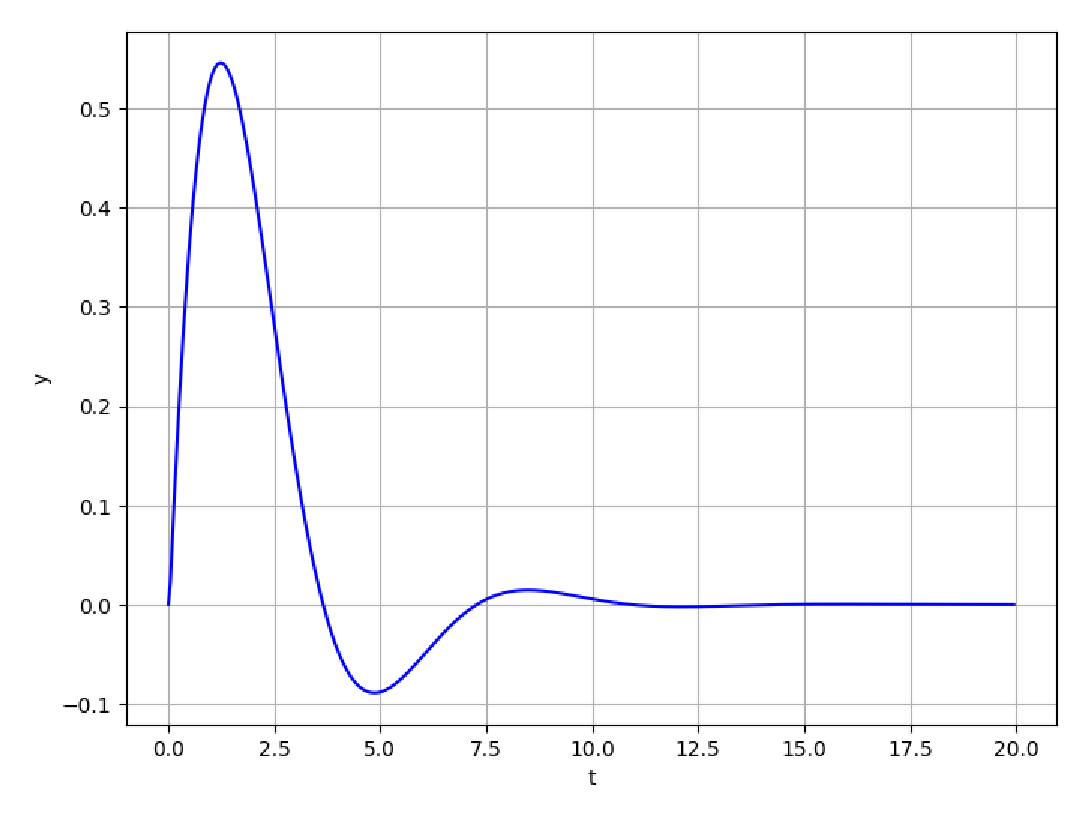
\includegraphics[scale=0.05]{figure3.eps}
    \end{minipage}
    \begin{minipage}[h]{0.5\linewidth}
      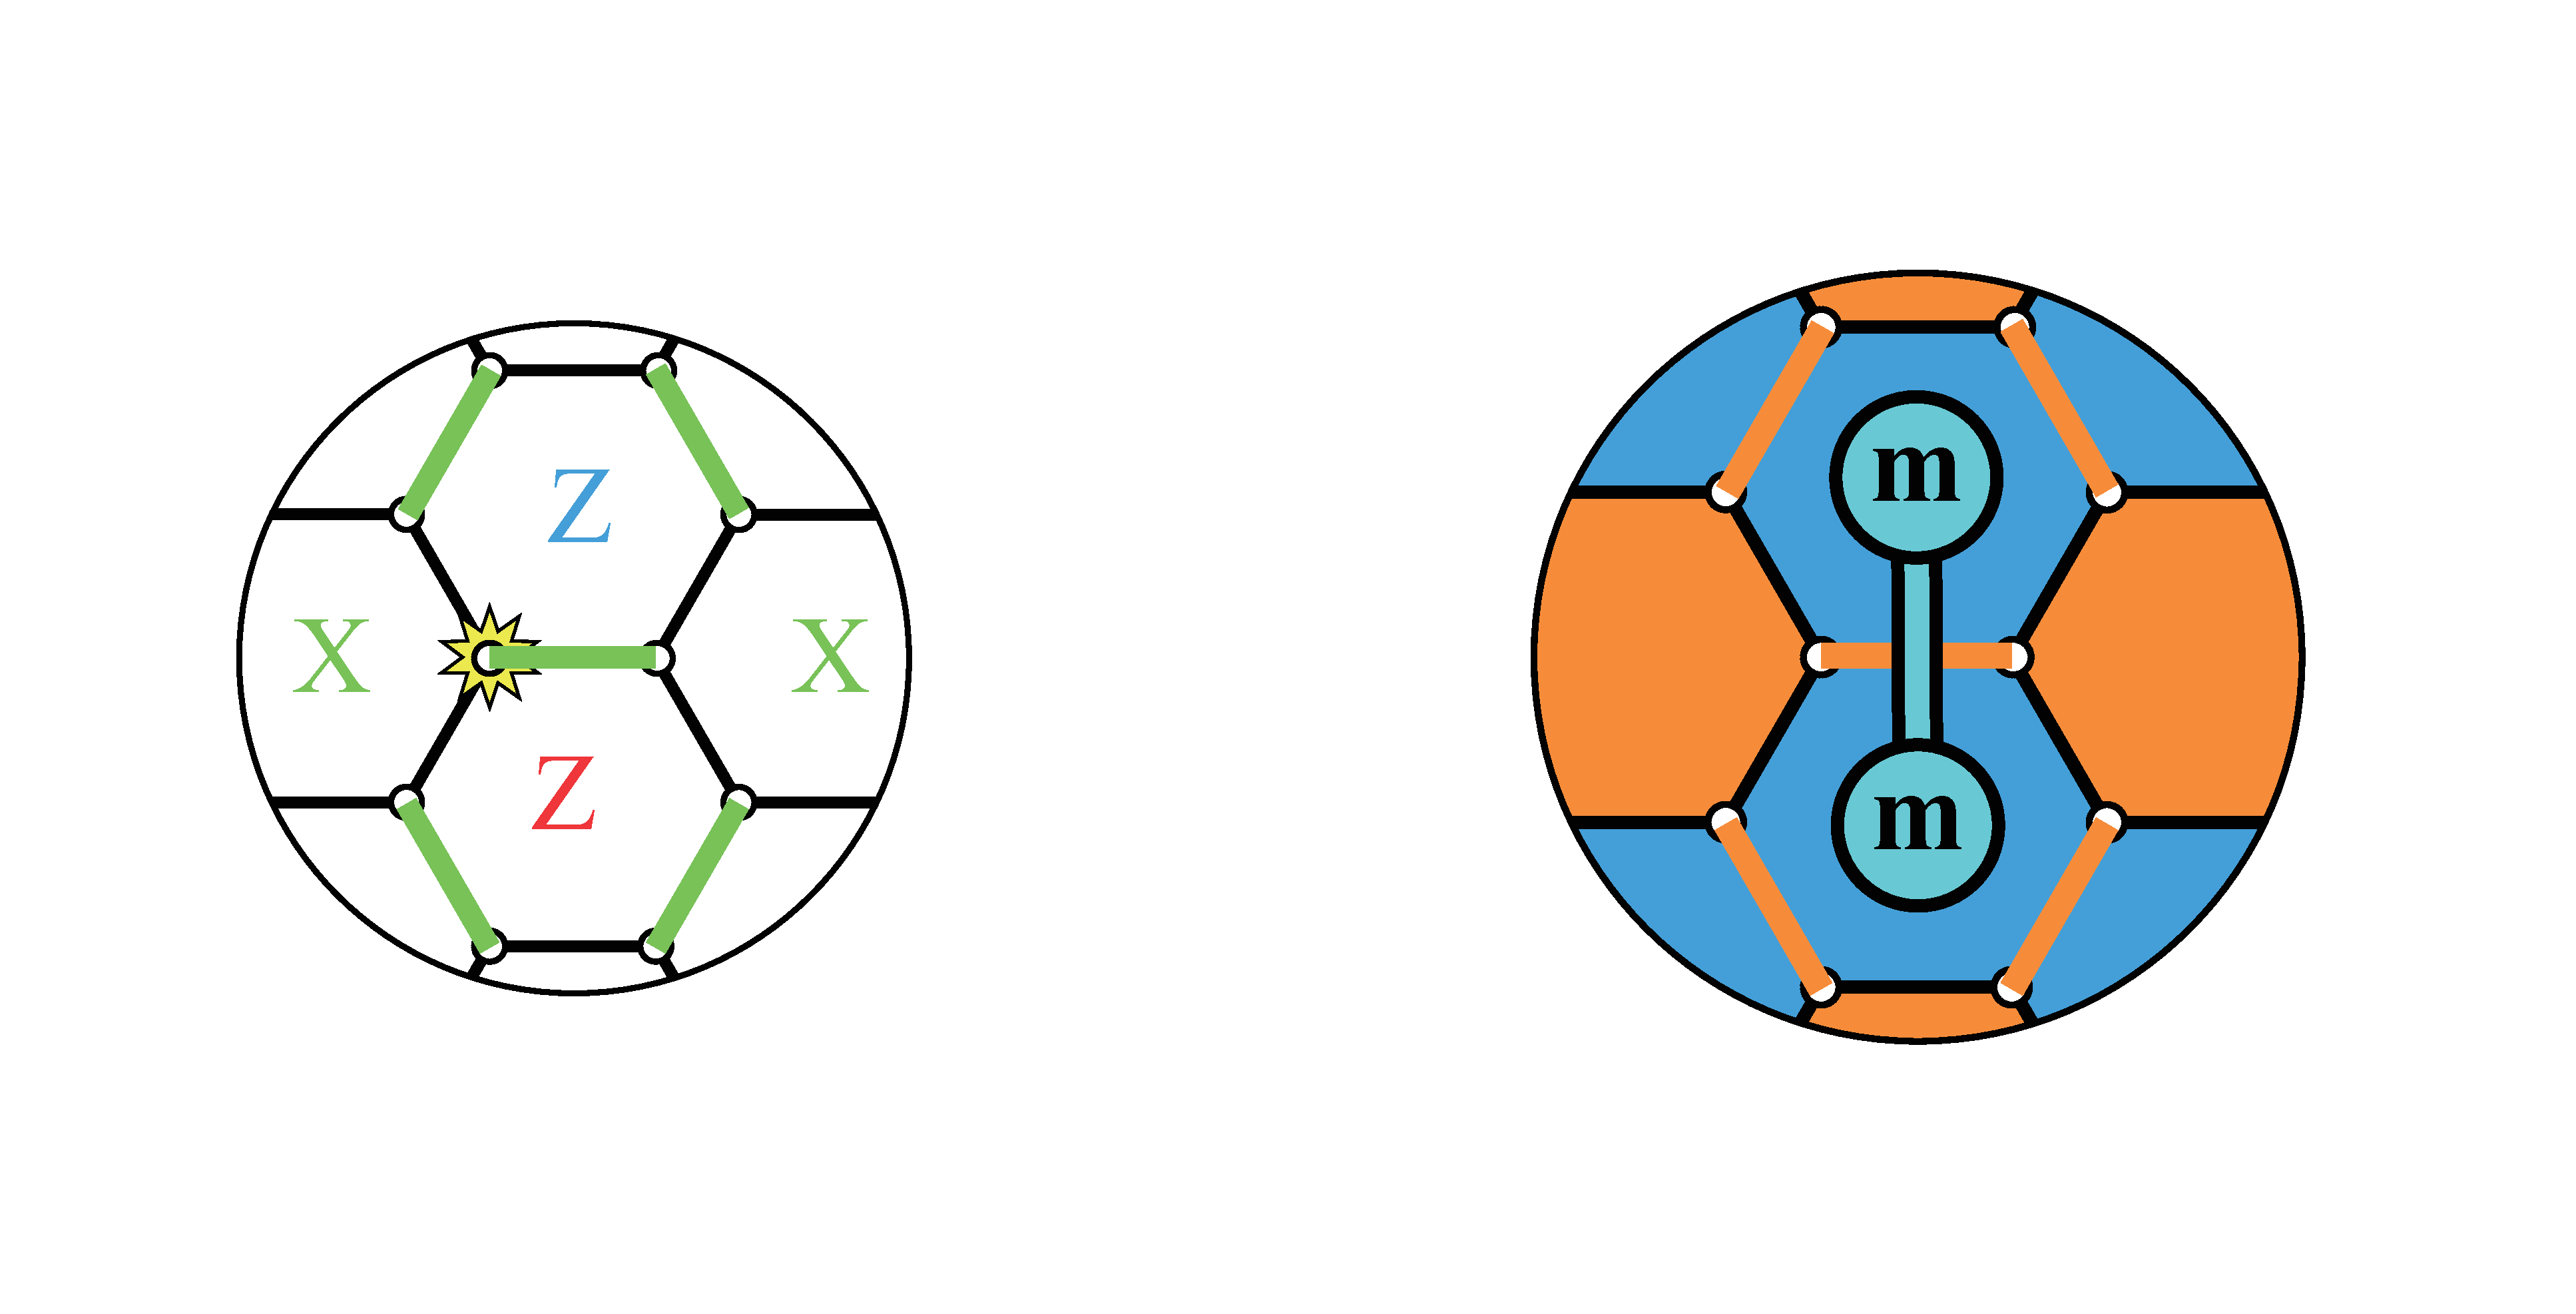
\includegraphics[scale=0.05]{figure4.eps}
    \end{minipage}
    \caption*{(a)}
  \end{minipage}
  \begin{minipage}[h]{0.8\linewidth}
    \begin{minipage}[h]{0.53\linewidth}
      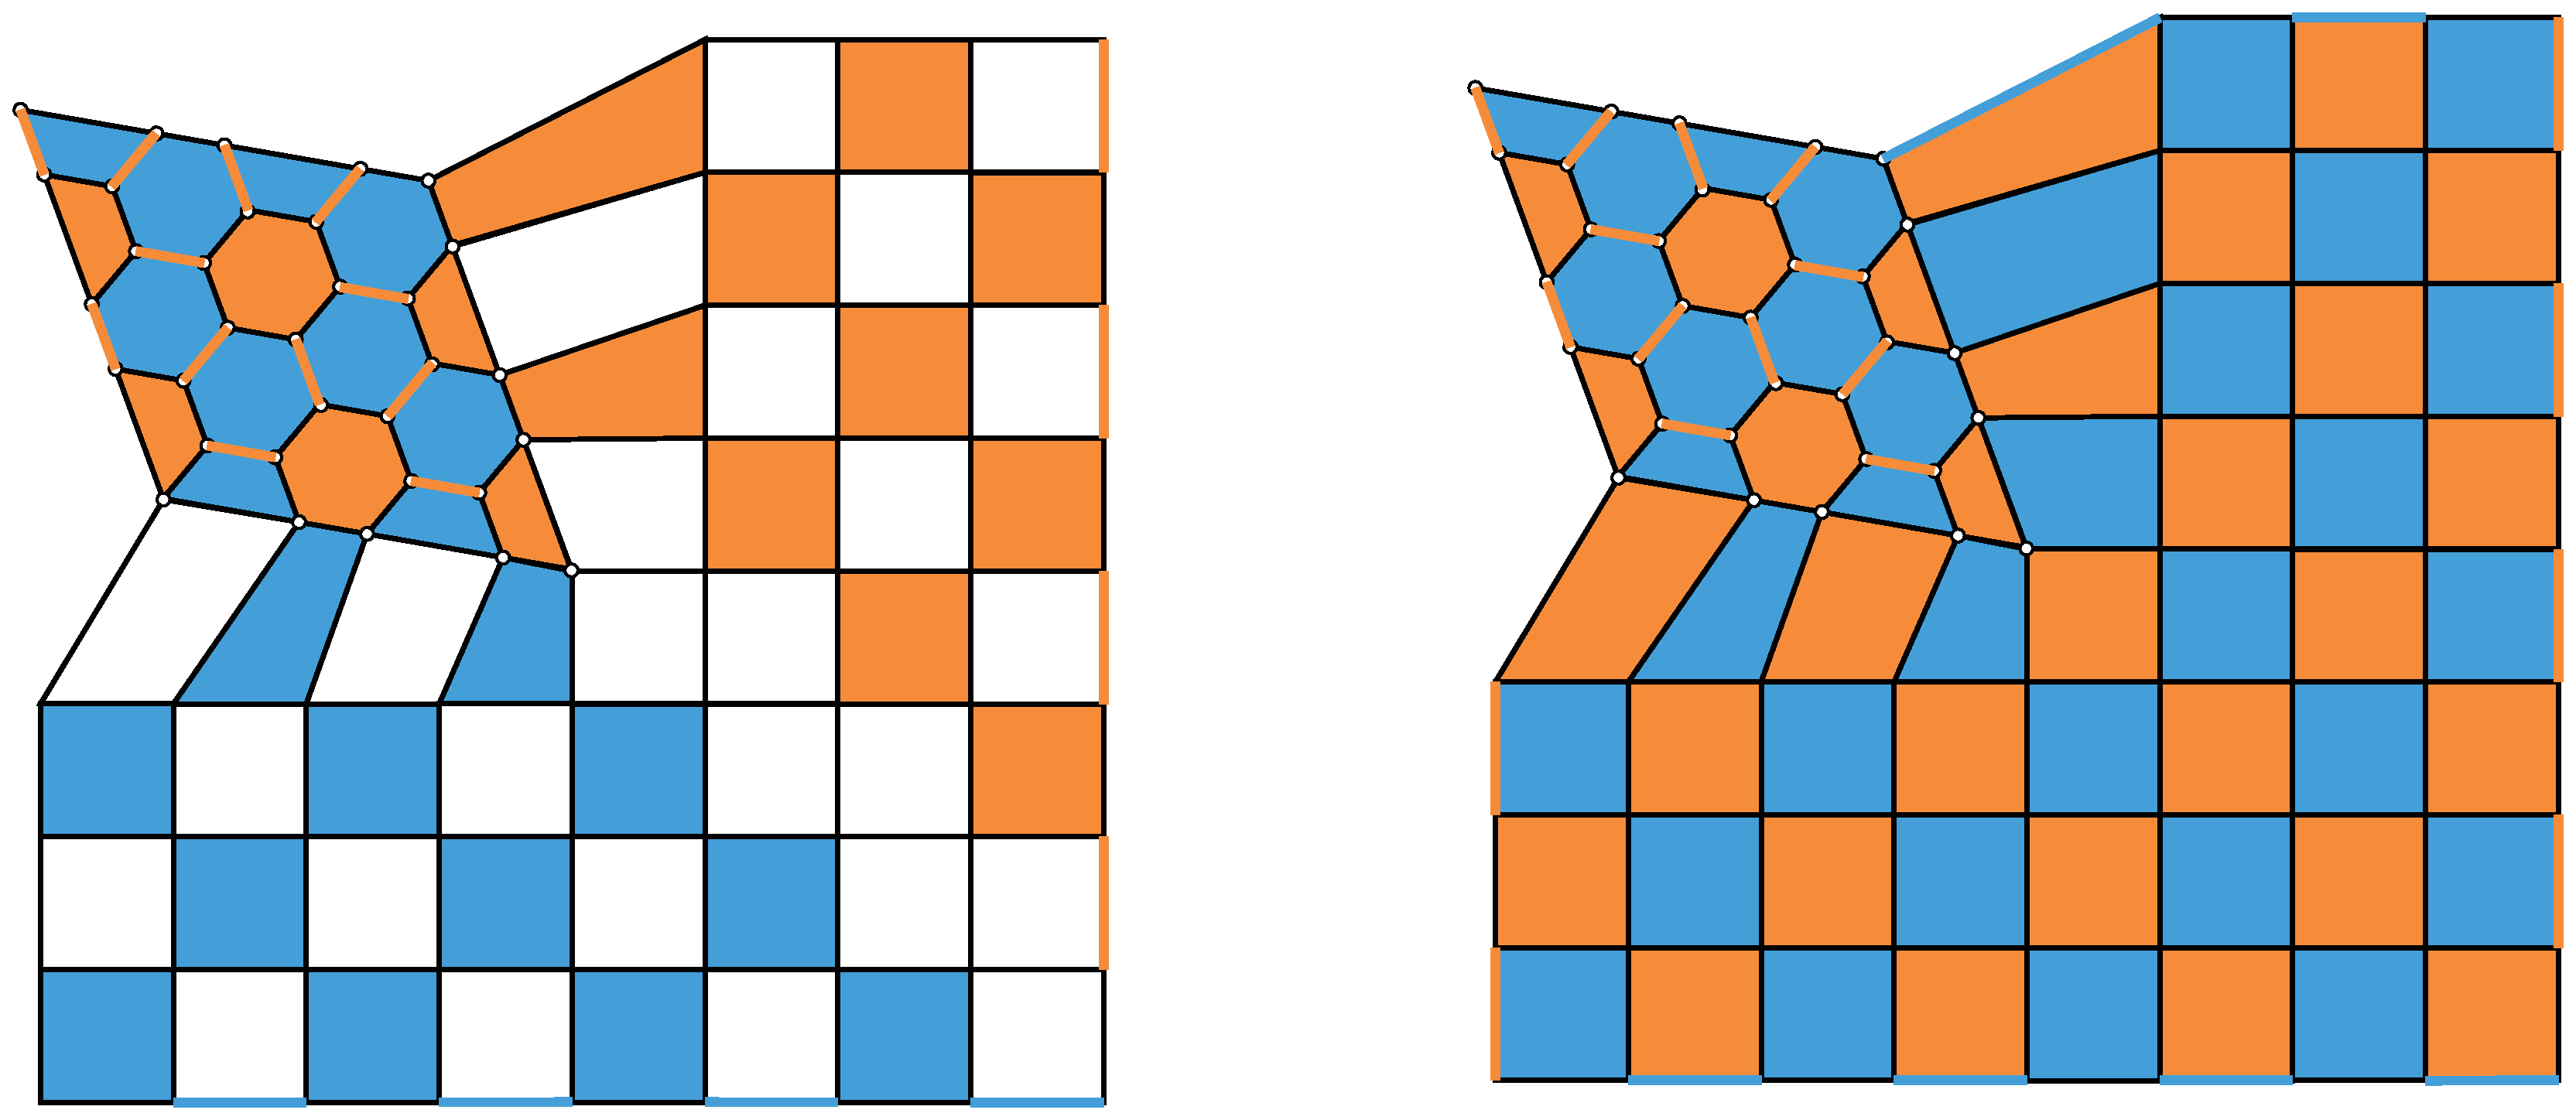
\includegraphics[scale=0.05]{figure5.eps}
    \end{minipage}
    \begin{minipage}[h]{0.5\linewidth}
      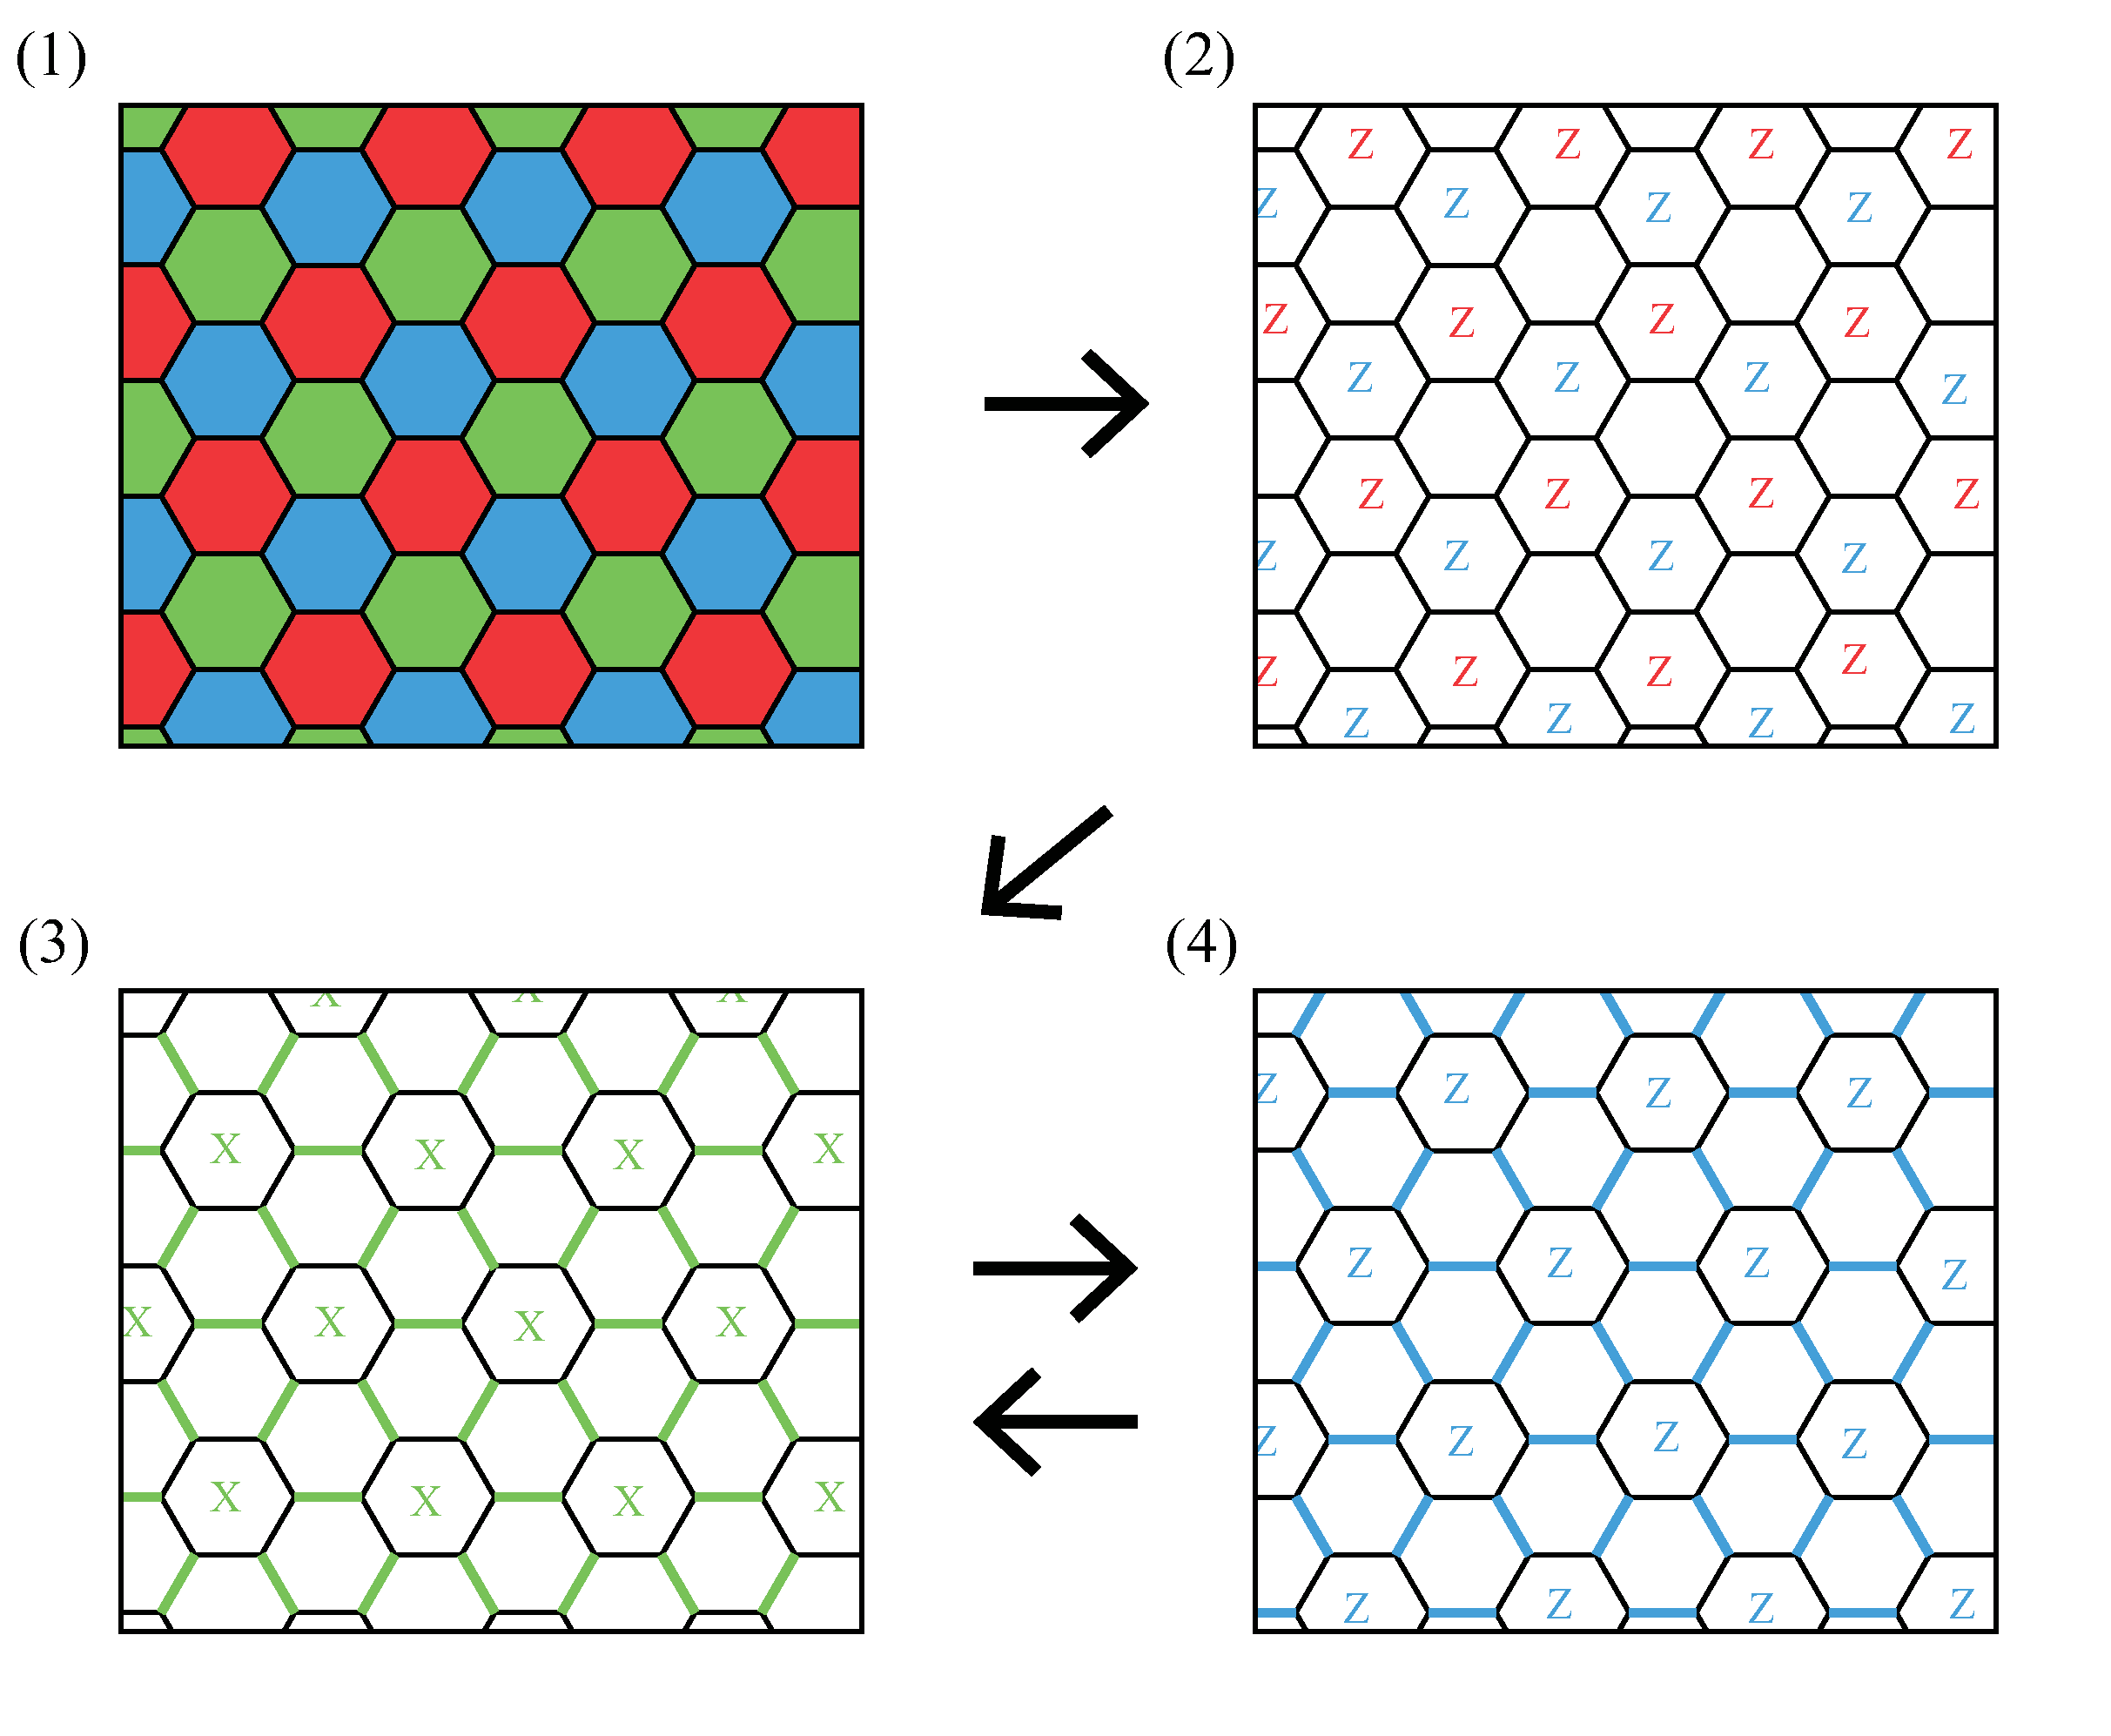
\includegraphics[scale=0.05]{figure6.eps}
    \end{minipage}
    \caption*{(b)}
  \end{minipage}
  \begin{minipage}[h]{0.8\linewidth}
    \begin{minipage}[h]{0.53\linewidth}
      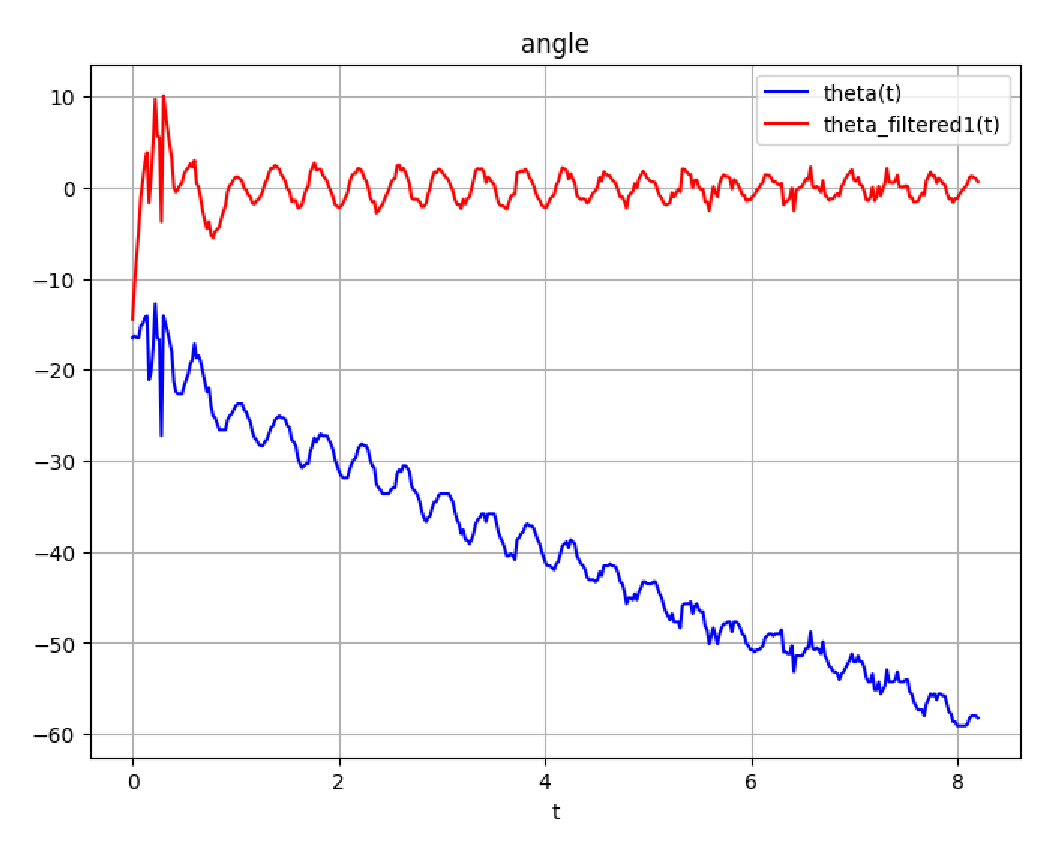
\includegraphics[scale=0.05]{figure7.eps}
    \end{minipage}
    \begin{minipage}[h]{0.5\linewidth}
      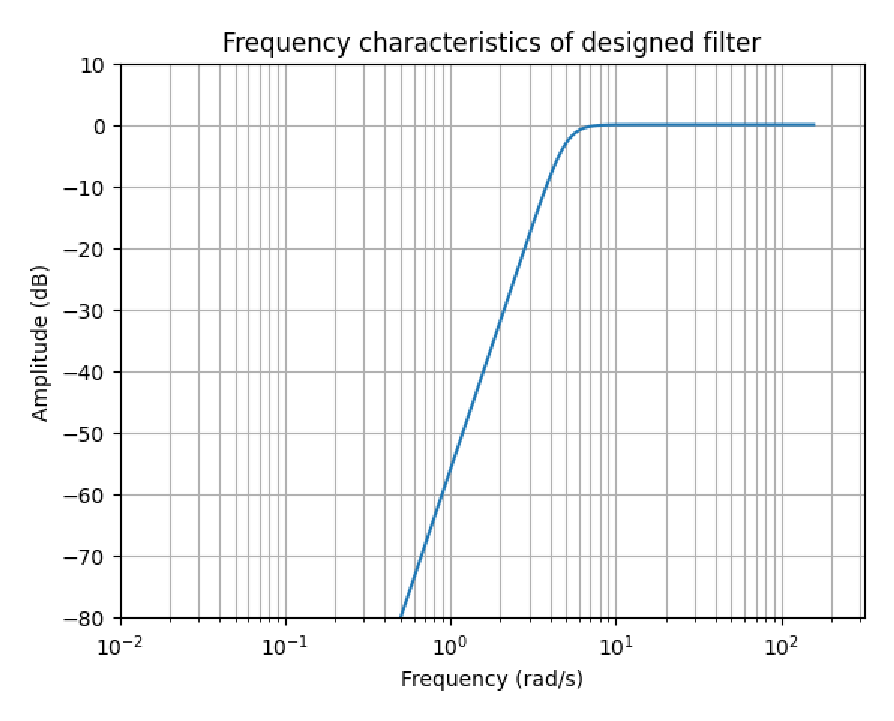
\includegraphics[scale=0.05]{figure8.eps}
    \end{minipage}
    \caption*{(c)}
  \end{minipage}
  \caption{オシロスコープ(a)白色の光ファイバー、(b)橙色の光ファイバー、(c)水色の光ファイバー}
  \label{scope}
\end{figure}
\clearpage
\hspace{-2pt}{\Large \bfseries 3.考察}\\
{\large \bfseries 3.1光ファイバの種類と構造}\\
 光ファイバの種類には、シングルモードファイバ、SI型のマルチモードファイバ、GI型のマルチモードファイバが存在する。シングルモードファイバはコア径が$8〜10\ \mathrm{\upmu m}$で小さく、単一方向つまり光ファイバーに平行な向きの光しか伝送できない。しかし、シングルモードの光しか伝送できないことから原理的にモード分散が存在せず、長距離の光伝送に向いている。マルチモードファイバはコア径が$50〜62.5\ \mathrm{\upmu m}$である。このうち、SI型はコア全体の屈折率が一定で入射した光はコアとクラッドの境目で全反射を繰り返しながら伝送される。また、コア径が大きいため複数の方向の光を伝送することができる。しかし、クラッドへの入射が小さい光は光路長がクラッドへの入射角が大きい光より長くなり、モード分散が大きくなる。これを改善するために作られた光ファイバがGI型のマルチモードファイバで、SI型と違ってコアの屈折率が中心から外側に向かって小さくなるようになっている。これにより、クラッドへの入射角の大きい光は屈折率の大きい領域を通過する時間が長くなり、逆にクラッドへの入射角の小さい光は屈折率の大きい領域と小さい領域を通り、最終的にどのモードの光も同じぐらいのタイミングで伝送先へ到着する。そのため、GI型はモード分散が小さい。このようなことから、シングルモードファイバは大陸間のような長距離の伝送、マルチモードファイバは家庭内のような短距離の伝送で用いられる。\\
\\
{\large \bfseries 3.2光結合特性}\\
 図\ref{core-efficiency}にコア面積と結合効率の関係を示す。ただし、点は表\ref{efficiency}での測定点、直線はそれらの回帰直線を表す。
\begin{figure}[h]
  \centering
  \scalebox{0.5}[0.5]{
\begin{tikzpicture}[gnuplot]
%% generated with GNUPLOT 5.4p10 (Lua 5.4; terminal rev. Jun 2020, script rev. 118)
%% Mon Dec 11 14:39:44 2023
\path (0.000,0.000) rectangle (12.500,8.750);
\gpcolor{color=gp lt color border}
\gpsetlinetype{gp lt border}
\gpsetdashtype{gp dt solid}
\gpsetlinewidth{1.00}
\draw[gp path] (0.018,0.031)--(0.198,0.031);
\draw[gp path] (12.480,0.031)--(12.300,0.031);
\node[gp node right] at (-0.166,0.031) {$0$};
\draw[gp path] (0.018,1.768)--(0.198,1.768);
\draw[gp path] (12.480,1.768)--(12.300,1.768);
\node[gp node right] at (-0.166,1.768) {$2$};
\draw[gp path] (0.018,3.506)--(0.198,3.506);
\draw[gp path] (12.480,3.506)--(12.300,3.506);
\node[gp node right] at (-0.166,3.506) {$4$};
\draw[gp path] (0.018,5.243)--(0.198,5.243);
\draw[gp path] (12.480,5.243)--(12.300,5.243);
\node[gp node right] at (-0.166,5.243) {$6$};
\draw[gp path] (0.018,6.981)--(0.198,6.981);
\draw[gp path] (12.480,6.981)--(12.300,6.981);
\node[gp node right] at (-0.166,6.981) {$8$};
\draw[gp path] (0.018,8.718)--(0.198,8.718);
\draw[gp path] (12.480,8.718)--(12.300,8.718);
\node[gp node right] at (-0.166,8.718) {$10$};
\draw[gp path] (0.018,0.031)--(0.018,0.211);
\draw[gp path] (0.018,8.718)--(0.018,8.538);
\node[gp node center] at (0.018,-0.277) {$0$};
\draw[gp path] (1.798,0.031)--(1.798,0.211);
\draw[gp path] (1.798,8.718)--(1.798,8.538);
\node[gp node center] at (1.798,-0.277) {$20000$};
\draw[gp path] (3.579,0.031)--(3.579,0.211);
\draw[gp path] (3.579,8.718)--(3.579,8.538);
\node[gp node center] at (3.579,-0.277) {$40000$};
\draw[gp path] (5.359,0.031)--(5.359,0.211);
\draw[gp path] (5.359,8.718)--(5.359,8.538);
\node[gp node center] at (5.359,-0.277) {$60000$};
\draw[gp path] (7.139,0.031)--(7.139,0.211);
\draw[gp path] (7.139,8.718)--(7.139,8.538);
\node[gp node center] at (7.139,-0.277) {$80000$};
\draw[gp path] (8.919,0.031)--(8.919,0.211);
\draw[gp path] (8.919,8.718)--(8.919,8.538);
\node[gp node center] at (8.919,-0.277) {$100000$};
\draw[gp path] (10.700,0.031)--(10.700,0.211);
\draw[gp path] (10.700,8.718)--(10.700,8.538);
\node[gp node center] at (10.700,-0.277) {$120000$};
\draw[gp path] (12.480,0.031)--(12.480,0.211);
\draw[gp path] (12.480,8.718)--(12.480,8.538);
\node[gp node center] at (12.480,-0.277) {$140000$};
\draw[gp path] (0.018,8.718)--(0.018,0.031)--(12.480,0.031)--(12.480,8.718)--cycle;
\node[gp node center,rotate=-270,font={\fontsize{17.0pt}{20.4pt}\selectfont}] at (-1.102,4.374) {結合効率$\ /\ \%$};
\node[gp node center,font={\fontsize{17.0pt}{20.4pt}\selectfont}] at (6.249,-1.046) {コア面積$\ /\ \mathrm{\upmu m^2}$};
\gpcolor{rgb color={0.000,0.000,0.000}}
\gpsetpointsize{4.00}
\gp3point{gp mark 7}{}{(0.046,0.062)}
\gp3point{gp mark 7}{}{(0.717,0.537)}
\gp3point{gp mark 7}{}{(11.204,7.779)}
\gpsetlinewidth{2.00}
\draw[gp path] (0.018,0.048)--(0.144,0.135)--(0.270,0.222)--(0.396,0.309)--(0.522,0.396)%
  --(0.647,0.483)--(0.773,0.570)--(0.899,0.657)--(1.025,0.744)--(1.151,0.831)--(1.277,0.918)%
  --(1.403,1.005)--(1.529,1.092)--(1.654,1.179)--(1.780,1.266)--(1.906,1.353)--(2.032,1.440)%
  --(2.158,1.527)--(2.284,1.614)--(2.410,1.701)--(2.536,1.788)--(2.661,1.875)--(2.787,1.962)%
  --(2.913,2.049)--(3.039,2.136)--(3.165,2.223)--(3.291,2.310)--(3.417,2.397)--(3.543,2.484)%
  --(3.668,2.571)--(3.794,2.658)--(3.920,2.745)--(4.046,2.832)--(4.172,2.919)--(4.298,3.006)%
  --(4.424,3.093)--(4.550,3.180)--(4.676,3.267)--(4.801,3.354)--(4.927,3.441)--(5.053,3.528)%
  --(5.179,3.615)--(5.305,3.702)--(5.431,3.789)--(5.557,3.876)--(5.683,3.963)--(5.808,4.050)%
  --(5.934,4.137)--(6.060,4.224)--(6.186,4.311)--(6.312,4.398)--(6.438,4.485)--(6.564,4.572)%
  --(6.690,4.659)--(6.815,4.746)--(6.941,4.833)--(7.067,4.920)--(7.193,5.007)--(7.319,5.094)%
  --(7.445,5.181)--(7.571,5.268)--(7.697,5.355)--(7.822,5.442)--(7.948,5.529)--(8.074,5.616)%
  --(8.200,5.703)--(8.326,5.790)--(8.452,5.877)--(8.578,5.964)--(8.704,6.051)--(8.830,6.138)%
  --(8.955,6.225)--(9.081,6.312)--(9.207,6.399)--(9.333,6.486)--(9.459,6.573)--(9.585,6.660)%
  --(9.711,6.747)--(9.837,6.834)--(9.962,6.921)--(10.088,7.008)--(10.214,7.095)--(10.340,7.182)%
  --(10.466,7.269)--(10.592,7.356)--(10.718,7.443)--(10.844,7.530)--(10.969,7.617)--(11.095,7.704)%
  --(11.221,7.791)--(11.347,7.878)--(11.473,7.965)--(11.599,8.052)--(11.725,8.139)--(11.851,8.226)%
  --(11.976,8.313)--(12.102,8.400)--(12.228,8.487)--(12.354,8.574)--(12.480,8.661);
\gpcolor{color=gp lt color border}
\gpsetlinewidth{1.00}
\draw[gp path] (0.018,8.718)--(0.018,0.031)--(12.480,0.031)--(12.480,8.718)--cycle;
%% coordinates of the plot area
\gpdefrectangularnode{gp plot 1}{\pgfpoint{0.018cm}{0.031cm}}{\pgfpoint{12.480cm}{8.718cm}}
\end{tikzpicture}
}

  \vspace{-30pt}\caption{コア面積と結合効率の関係}
  \label{core-efficiency}
\end{figure}
これより、グラフの直線の方程式は傾きが$7.08\times 10^{-5}$、切片が$0.0197$である。今、結合効率を$100\ \%$とすることを考えると、コア径は$670\ \mathrm{\upmu m}$である必要がある。ただし、図\ref{core-efficiency}の回帰直線での近似はコア面積が小さい範囲でしか成り立たないと考えられるから、実際は上記で求めた値は必ずしも正しくない。\\
\\
{\large \bfseries 3.3伝送損失}\\
  文献\cite{text}の(2)式から、$P$とそれよりも少し大きい$P+\Delta P$、光強度が$P$のときの光ファイバの長さを$L$、光強度が$P+\Delta L$のときの光ファイバの長さを$L+\Delta L$とすると、伝送損失$T$は、
\begin{align}
  T&=-\frac{10}{\Delta L}\log{\frac{P+\Delta P}{P}}\nonumber\\[10pt]
  &=-\frac{10\log{(P+\Delta P)}-10\log{P}}{\Delta L}
\end{align}
となる。これより、伝送損失$T$は図\ref{loss}の2つの点を結んだ直線の傾きに$-1$を掛けた値だとわかる。また、$L=0$としたとき、接続損失のみによってレーザから出射された光が失われるから、このとき観測される光強度は光ファイバーに入射した光強度であることがわかる。\\
 また、文献\cite{text}の図4から伝送損失は約$18\ \mathrm{dB/km}$である。よって、2.2節で求めた伝送損失$44\ \mathrm{dB/km}$は大きな誤差を持つ。誤差の原因として考えられるのは、実験の際、レーザと測定装置の他にも$100,60,10,1 \mathrm{m}$の光ファイバーの接続部分があったことである。これにより、多くの接続損失が生み出され文献値よりも実験値の方が伝送損失が大きくなったのだと考えられる。
\clearpage
{\large \bfseries 3.4マルチモードファイバの屈折率分布}\\
 まず、文献\cite{text}の(9)式から、
\begin{align}
  n(r)&=\frac{P(r)}{P(0)}\left\{n(0)-n_2\right\}+n_2\nonumber\\[10pt]
  &=\frac{P(r)}{P(0)}\frac{\Delta}{1-\Delta}n_2+n_2\nonumber\\[10pt]
  &=0.1618\frac{P(r)}{P(0)}+1.457
\end{align}
となる。ただし、$\Delta=0.01\ ,\ n_2=1.457$を用いた。よって、(2)式を用いると図\ref{GI}(b)は図\ref{GIfixed}、図\ref{SI} (b)は図\ref{SIfixed}となる。\\
\begin{figure}[h]
  \centering
  \scalebox{0.5}[0.5]{
\begin{tikzpicture}[gnuplot]
%% generated with GNUPLOT 5.4p10 (Lua 5.4; terminal rev. Jun 2020, script rev. 118)
%% Sun Dec  3 22:55:04 2023
\path (0.000,0.000) rectangle (12.500,8.750);
\gpcolor{color=gp lt color border}
\gpsetlinetype{gp lt border}
\gpsetdashtype{gp dt solid}
\gpsetlinewidth{1.00}
\draw[gp path] (0.018,0.031)--(0.198,0.031);
\draw[gp path] (12.480,0.031)--(12.300,0.031);
\node[gp node right] at (-0.166,0.031) {$480$};
\draw[gp path] (0.018,0.900)--(0.198,0.900);
\draw[gp path] (12.480,0.900)--(12.300,0.900);
\node[gp node right] at (-0.166,0.900) {$490$};
\draw[gp path] (0.018,1.768)--(0.198,1.768);
\draw[gp path] (12.480,1.768)--(12.300,1.768);
\node[gp node right] at (-0.166,1.768) {$500$};
\draw[gp path] (0.018,2.637)--(0.198,2.637);
\draw[gp path] (12.480,2.637)--(12.300,2.637);
\node[gp node right] at (-0.166,2.637) {$510$};
\draw[gp path] (0.018,3.506)--(0.198,3.506);
\draw[gp path] (12.480,3.506)--(12.300,3.506);
\node[gp node right] at (-0.166,3.506) {$520$};
\draw[gp path] (0.018,4.375)--(0.198,4.375);
\draw[gp path] (12.480,4.375)--(12.300,4.375);
\node[gp node right] at (-0.166,4.375) {$530$};
\draw[gp path] (0.018,5.243)--(0.198,5.243);
\draw[gp path] (12.480,5.243)--(12.300,5.243);
\node[gp node right] at (-0.166,5.243) {$540$};
\draw[gp path] (0.018,6.112)--(0.198,6.112);
\draw[gp path] (12.480,6.112)--(12.300,6.112);
\node[gp node right] at (-0.166,6.112) {$550$};
\draw[gp path] (0.018,6.981)--(0.198,6.981);
\draw[gp path] (12.480,6.981)--(12.300,6.981);
\node[gp node right] at (-0.166,6.981) {$560$};
\draw[gp path] (0.018,7.849)--(0.198,7.849);
\draw[gp path] (12.480,7.849)--(12.300,7.849);
\node[gp node right] at (-0.166,7.849) {$570$};
\draw[gp path] (0.018,8.718)--(0.198,8.718);
\draw[gp path] (12.480,8.718)--(12.300,8.718);
\node[gp node right] at (-0.166,8.718) {$580$};
\draw[gp path] (0.018,0.031)--(0.018,0.211);
\draw[gp path] (0.018,8.718)--(0.018,8.538);
\node[gp node center] at (0.018,-0.277) {$-0.5$};
\draw[gp path] (1.576,0.031)--(1.576,0.211);
\draw[gp path] (1.576,8.718)--(1.576,8.538);
\node[gp node center] at (1.576,-0.277) {$0$};
\draw[gp path] (3.134,0.031)--(3.134,0.211);
\draw[gp path] (3.134,8.718)--(3.134,8.538);
\node[gp node center] at (3.134,-0.277) {$0.5$};
\draw[gp path] (4.691,0.031)--(4.691,0.211);
\draw[gp path] (4.691,8.718)--(4.691,8.538);
\node[gp node center] at (4.691,-0.277) {$1$};
\draw[gp path] (6.249,0.031)--(6.249,0.211);
\draw[gp path] (6.249,8.718)--(6.249,8.538);
\node[gp node center] at (6.249,-0.277) {$1.5$};
\draw[gp path] (7.807,0.031)--(7.807,0.211);
\draw[gp path] (7.807,8.718)--(7.807,8.538);
\node[gp node center] at (7.807,-0.277) {$2$};
\draw[gp path] (9.365,0.031)--(9.365,0.211);
\draw[gp path] (9.365,8.718)--(9.365,8.538);
\node[gp node center] at (9.365,-0.277) {$2.5$};
\draw[gp path] (10.922,0.031)--(10.922,0.211);
\draw[gp path] (10.922,8.718)--(10.922,8.538);
\node[gp node center] at (10.922,-0.277) {$3$};
\draw[gp path] (12.480,0.031)--(12.480,0.211);
\draw[gp path] (12.480,8.718)--(12.480,8.538);
\node[gp node center] at (12.480,-0.277) {$3.5$};
\draw[gp path] (0.018,8.718)--(0.018,0.031)--(12.480,0.031)--(12.480,8.718)--cycle;
\node[gp node center,rotate=-270,font={\fontsize{17.0pt}{20.4pt}\selectfont}] at (-1.286,4.374) {$C_k$};
\node[gp node center,font={\fontsize{17.0pt}{20.4pt}\selectfont}] at (6.249,-1.046) {$k$};
\gpcolor{rgb color={0.000,0.000,0.000}}
\draw[gp path] (1.576,5.183)--(4.691,7.981)--(7.807,6.092)--(10.922,0.744);
\gpsetpointsize{1.20}
\gp3point{gp mark 7}{}{(1.576,5.183)}
\gp3point{gp mark 7}{}{(4.691,7.981)}
\gp3point{gp mark 7}{}{(7.807,6.092)}
\gp3point{gp mark 7}{}{(10.922,0.744)}
\gpcolor{color=gp lt color border}
\draw[gp path] (0.018,8.718)--(0.018,0.031)--(12.480,0.031)--(12.480,8.718)--cycle;
%% coordinates of the plot area
\gpdefrectangularnode{gp plot 1}{\pgfpoint{0.018cm}{0.031cm}}{\pgfpoint{12.480cm}{8.718cm%% gnuplot variables
}

  \vspace{-30pt}\caption{GI型の屈折率分布}
  \label{GIfixed}
\end{figure}
\begin{figure}[h]
  \centering
  \scalebox{0.7}[0.7]{
\begin{tikzpicture}[gnuplot]
%% generated with GNUPLOT 5.4p10 (Lua 5.4; terminal rev. Jun 2020, script rev. 118)
%% Mon Dec 11 22:23:16 2023
\path (0.000,0.000) rectangle (12.500,8.750);
\gpcolor{color=gp lt color border}
\gpsetlinetype{gp lt border}
\gpsetdashtype{gp dt solid}
\gpsetlinewidth{1.00}
\draw[gp path] (0.018,0.031)--(0.198,0.031);
\draw[gp path] (12.480,0.031)--(12.300,0.031);
\node[gp node right] at (-0.166,0.031) {$1.46$};
\draw[gp path] (0.018,1.117)--(0.198,1.117);
\draw[gp path] (12.480,1.117)--(12.300,1.117);
\node[gp node right] at (-0.166,1.117) {$1.48$};
\draw[gp path] (0.018,2.203)--(0.198,2.203);
\draw[gp path] (12.480,2.203)--(12.300,2.203);
\node[gp node right] at (-0.166,2.203) {$1.5$};
\draw[gp path] (0.018,3.289)--(0.198,3.289);
\draw[gp path] (12.480,3.289)--(12.300,3.289);
\node[gp node right] at (-0.166,3.289) {$1.52$};
\draw[gp path] (0.018,4.375)--(0.198,4.375);
\draw[gp path] (12.480,4.375)--(12.300,4.375);
\node[gp node right] at (-0.166,4.375) {$1.54$};
\draw[gp path] (0.018,5.460)--(0.198,5.460);
\draw[gp path] (12.480,5.460)--(12.300,5.460);
\node[gp node right] at (-0.166,5.460) {$1.56$};
\draw[gp path] (0.018,6.546)--(0.198,6.546);
\draw[gp path] (12.480,6.546)--(12.300,6.546);
\node[gp node right] at (-0.166,6.546) {$1.58$};
\draw[gp path] (0.018,7.632)--(0.198,7.632);
\draw[gp path] (12.480,7.632)--(12.300,7.632);
\node[gp node right] at (-0.166,7.632) {$1.6$};
\draw[gp path] (0.018,8.718)--(0.198,8.718);
\draw[gp path] (12.480,8.718)--(12.300,8.718);
\node[gp node right] at (-0.166,8.718) {$1.62$};
\draw[gp path] (0.018,0.031)--(0.018,0.211);
\draw[gp path] (0.018,8.718)--(0.018,8.538);
\node[gp node center] at (0.018,-0.277) {$-150$};
\draw[gp path] (2.095,0.031)--(2.095,0.211);
\draw[gp path] (2.095,8.718)--(2.095,8.538);
\node[gp node center] at (2.095,-0.277) {$-100$};
\draw[gp path] (4.172,0.031)--(4.172,0.211);
\draw[gp path] (4.172,8.718)--(4.172,8.538);
\node[gp node center] at (4.172,-0.277) {$-50$};
\draw[gp path] (6.249,0.031)--(6.249,0.211);
\draw[gp path] (6.249,8.718)--(6.249,8.538);
\node[gp node center] at (6.249,-0.277) {$0$};
\draw[gp path] (8.326,0.031)--(8.326,0.211);
\draw[gp path] (8.326,8.718)--(8.326,8.538);
\node[gp node center] at (8.326,-0.277) {$50$};
\draw[gp path] (10.403,0.031)--(10.403,0.211);
\draw[gp path] (10.403,8.718)--(10.403,8.538);
\node[gp node center] at (10.403,-0.277) {$100$};
\draw[gp path] (12.480,0.031)--(12.480,0.211);
\draw[gp path] (12.480,8.718)--(12.480,8.538);
\node[gp node center] at (12.480,-0.277) {$150$};
\draw[gp path] (0.018,8.718)--(0.018,0.031)--(12.480,0.031)--(12.480,8.718)--cycle;
\node[gp node center,rotate=-270,font={\fontsize{17.0pt}{20.4pt}\selectfont}] at (-1.470,4.374) {屈折率$n(r)$};
\node[gp node center,font={\fontsize{17.0pt}{20.4pt}\selectfont}] at (6.249,-1.046) {中心からの距離$r\ /\ \mathrm{\upmu m}$};
\gpcolor{rgb color={0.000,0.000,0.000}}
\draw[gp path] (0.018,0.255)--(0.056,0.287)--(0.118,0.282)--(0.179,0.273)--(0.240,0.304)%
  --(0.302,0.247)--(0.363,0.287)--(0.424,0.335)--(0.486,0.287)--(0.547,0.278)--(0.608,0.295)%
  --(0.670,0.331)--(0.731,0.300)--(0.792,0.278)--(0.853,0.273)--(0.915,0.247)--(0.976,0.243)%
  --(1.037,0.326)--(1.099,0.243)--(1.160,0.282)--(1.221,0.260)--(1.283,0.313)--(1.344,0.340)%
  --(1.405,0.278)--(1.467,0.317)--(1.528,0.273)--(1.589,0.313)--(1.651,0.344)--(1.712,0.326)%
  --(1.773,0.295)--(1.834,0.295)--(1.896,0.313)--(1.957,0.375)--(2.018,0.335)--(2.080,0.375)%
  --(2.141,0.375)--(2.202,0.366)--(2.264,0.357)--(2.325,0.414)--(2.386,0.480)--(2.448,0.533)%
  --(2.509,0.617)--(2.570,0.683)--(2.632,0.802)--(2.693,1.014)--(2.754,1.353)--(2.815,1.732)%
  --(2.877,2.529)--(2.938,3.177)--(2.999,3.459)--(3.061,3.860)--(3.122,4.335)--(3.183,5.172)%
  --(3.245,5.644)--(3.306,6.093)--(3.367,6.318)--(3.429,6.943)--(3.490,7.177)--(3.551,7.239)%
  --(3.613,7.507)--(3.674,7.644)--(3.735,7.485)--(3.796,7.736)--(3.858,7.754)--(3.919,7.939)%
  --(3.980,7.899)--(4.042,8.032)--(4.103,8.093)--(4.164,7.970)--(4.226,7.847)--(4.287,8.181)%
  --(4.348,7.877)--(4.410,7.996)--(4.471,8.040)--(4.532,8.212)--(4.594,7.781)--(4.655,8.221)%
  --(4.716,8.243)--(4.777,8.190)--(4.839,8.005)--(4.900,8.010)--(4.961,8.001)--(5.023,8.137)%
  --(5.084,8.102)--(5.145,8.327)--(5.207,8.151)--(5.268,8.195)--(5.329,8.256)--(5.391,8.093)%
  --(5.452,8.441)--(5.513,8.419)--(5.575,8.512)--(5.636,8.331)--(5.697,8.252)--(5.758,8.234)%
  --(5.820,8.344)--(5.881,8.181)--(5.942,8.159)--(6.004,8.287)--(6.065,8.415)--(6.126,8.384)%
  --(6.188,8.503)--(6.249,8.653)--(6.310,8.569)--(6.372,8.393)--(6.433,8.309)--(6.494,8.375)%
  --(6.556,8.446)--(6.617,8.441)--(6.678,8.327)--(6.740,8.389)--(6.801,8.419)--(6.862,8.468)%
  --(6.923,8.626)--(6.985,8.534)--(7.046,8.507)--(7.107,8.248)--(7.169,8.362)--(7.230,8.433)%
  --(7.291,8.450)--(7.353,8.283)--(7.414,8.578)--(7.475,8.212)--(7.537,8.371)--(7.598,8.468)%
  --(7.659,8.265)--(7.721,8.384)--(7.782,8.234)--(7.843,8.129)--(7.904,8.305)--(7.966,8.305)%
  --(8.027,8.274)--(8.088,8.168)--(8.150,8.296)--(8.211,8.190)--(8.272,8.120)--(8.334,8.155)%
  --(8.395,7.983)--(8.456,8.036)--(8.518,8.393)--(8.579,7.842)--(8.640,8.107)--(8.702,8.001)%
  --(8.763,7.944)--(8.824,8.133)--(8.885,8.212)--(8.947,8.089)--(9.008,7.895)--(9.069,8.278)%
  --(9.131,8.085)--(9.192,8.173)--(9.253,8.014)--(9.315,7.961)--(9.376,7.957)--(9.437,7.873)%
  --(9.499,7.750)--(9.560,8.102)--(9.621,7.833)--(9.683,7.754)--(9.744,7.551)--(9.805,7.195)%
  --(9.866,7.243)--(9.928,7.018)--(9.989,6.816)--(10.050,6.503)--(10.112,6.424)--(10.173,5.675)%
  --(10.234,5.349)--(10.296,4.688)--(10.357,3.494)--(10.418,2.419)--(10.480,1.890)--(10.541,1.463)%
  --(10.602,1.225)--(10.664,0.877)--(10.725,0.829)--(10.786,0.670)--(10.847,0.674)--(10.909,0.516)%
  --(10.970,0.454)--(11.031,0.414)--(11.093,0.344)--(11.154,0.370)--(11.215,0.370)--(11.277,0.348)%
  --(11.338,0.344)--(11.399,0.340)--(11.461,0.287)--(11.522,0.348)--(11.583,0.300)--(11.645,0.269)%
  --(11.706,0.282)--(11.767,0.295)--(11.828,0.317)--(11.890,0.353)--(11.951,0.326)--(12.012,0.265)%
  --(12.074,0.353)--(12.135,0.335)--(12.196,0.362)--(12.258,0.291)--(12.319,0.247)--(12.380,0.291)%
  --(12.442,0.269)--(12.480,0.315);
\gpsetpointsize{1.20}
\gp3point{gp mark 7}{}{(0.056,0.287)}
\gp3point{gp mark 7}{}{(0.118,0.282)}
\gp3point{gp mark 7}{}{(0.179,0.273)}
\gp3point{gp mark 7}{}{(0.240,0.304)}
\gp3point{gp mark 7}{}{(0.302,0.247)}
\gp3point{gp mark 7}{}{(0.363,0.287)}
\gp3point{gp mark 7}{}{(0.424,0.335)}
\gp3point{gp mark 7}{}{(0.486,0.287)}
\gp3point{gp mark 7}{}{(0.547,0.278)}
\gp3point{gp mark 7}{}{(0.608,0.295)}
\gp3point{gp mark 7}{}{(0.670,0.331)}
\gp3point{gp mark 7}{}{(0.731,0.300)}
\gp3point{gp mark 7}{}{(0.792,0.278)}
\gp3point{gp mark 7}{}{(0.853,0.273)}
\gp3point{gp mark 7}{}{(0.915,0.247)}
\gp3point{gp mark 7}{}{(0.976,0.243)}
\gp3point{gp mark 7}{}{(1.037,0.326)}
\gp3point{gp mark 7}{}{(1.099,0.243)}
\gp3point{gp mark 7}{}{(1.160,0.282)}
\gp3point{gp mark 7}{}{(1.221,0.260)}
\gp3point{gp mark 7}{}{(1.283,0.313)}
\gp3point{gp mark 7}{}{(1.344,0.340)}
\gp3point{gp mark 7}{}{(1.405,0.278)}
\gp3point{gp mark 7}{}{(1.467,0.317)}
\gp3point{gp mark 7}{}{(1.528,0.273)}
\gp3point{gp mark 7}{}{(1.589,0.313)}
\gp3point{gp mark 7}{}{(1.651,0.344)}
\gp3point{gp mark 7}{}{(1.712,0.326)}
\gp3point{gp mark 7}{}{(1.773,0.295)}
\gp3point{gp mark 7}{}{(1.834,0.295)}
\gp3point{gp mark 7}{}{(1.896,0.313)}
\gp3point{gp mark 7}{}{(1.957,0.375)}
\gp3point{gp mark 7}{}{(2.018,0.335)}
\gp3point{gp mark 7}{}{(2.080,0.375)}
\gp3point{gp mark 7}{}{(2.141,0.375)}
\gp3point{gp mark 7}{}{(2.202,0.366)}
\gp3point{gp mark 7}{}{(2.264,0.357)}
\gp3point{gp mark 7}{}{(2.325,0.414)}
\gp3point{gp mark 7}{}{(2.386,0.480)}
\gp3point{gp mark 7}{}{(2.448,0.533)}
\gp3point{gp mark 7}{}{(2.509,0.617)}
\gp3point{gp mark 7}{}{(2.570,0.683)}
\gp3point{gp mark 7}{}{(2.632,0.802)}
\gp3point{gp mark 7}{}{(2.693,1.014)}
\gp3point{gp mark 7}{}{(2.754,1.353)}
\gp3point{gp mark 7}{}{(2.815,1.732)}
\gp3point{gp mark 7}{}{(2.877,2.529)}
\gp3point{gp mark 7}{}{(2.938,3.177)}
\gp3point{gp mark 7}{}{(2.999,3.459)}
\gp3point{gp mark 7}{}{(3.061,3.860)}
\gp3point{gp mark 7}{}{(3.122,4.335)}
\gp3point{gp mark 7}{}{(3.183,5.172)}
\gp3point{gp mark 7}{}{(3.245,5.644)}
\gp3point{gp mark 7}{}{(3.306,6.093)}
\gp3point{gp mark 7}{}{(3.367,6.318)}
\gp3point{gp mark 7}{}{(3.429,6.943)}
\gp3point{gp mark 7}{}{(3.490,7.177)}
\gp3point{gp mark 7}{}{(3.551,7.239)}
\gp3point{gp mark 7}{}{(3.613,7.507)}
\gp3point{gp mark 7}{}{(3.674,7.644)}
\gp3point{gp mark 7}{}{(3.735,7.485)}
\gp3point{gp mark 7}{}{(3.796,7.736)}
\gp3point{gp mark 7}{}{(3.858,7.754)}
\gp3point{gp mark 7}{}{(3.919,7.939)}
\gp3point{gp mark 7}{}{(3.980,7.899)}
\gp3point{gp mark 7}{}{(4.042,8.032)}
\gp3point{gp mark 7}{}{(4.103,8.093)}
\gp3point{gp mark 7}{}{(4.164,7.970)}
\gp3point{gp mark 7}{}{(4.226,7.847)}
\gp3point{gp mark 7}{}{(4.287,8.181)}
\gp3point{gp mark 7}{}{(4.348,7.877)}
\gp3point{gp mark 7}{}{(4.410,7.996)}
\gp3point{gp mark 7}{}{(4.471,8.040)}
\gp3point{gp mark 7}{}{(4.532,8.212)}
\gp3point{gp mark 7}{}{(4.594,7.781)}
\gp3point{gp mark 7}{}{(4.655,8.221)}
\gp3point{gp mark 7}{}{(4.716,8.243)}
\gp3point{gp mark 7}{}{(4.777,8.190)}
\gp3point{gp mark 7}{}{(4.839,8.005)}
\gp3point{gp mark 7}{}{(4.900,8.010)}
\gp3point{gp mark 7}{}{(4.961,8.001)}
\gp3point{gp mark 7}{}{(5.023,8.137)}
\gp3point{gp mark 7}{}{(5.084,8.102)}
\gp3point{gp mark 7}{}{(5.145,8.327)}
\gp3point{gp mark 7}{}{(5.207,8.151)}
\gp3point{gp mark 7}{}{(5.268,8.195)}
\gp3point{gp mark 7}{}{(5.329,8.256)}
\gp3point{gp mark 7}{}{(5.391,8.093)}
\gp3point{gp mark 7}{}{(5.452,8.441)}
\gp3point{gp mark 7}{}{(5.513,8.419)}
\gp3point{gp mark 7}{}{(5.575,8.512)}
\gp3point{gp mark 7}{}{(5.636,8.331)}
\gp3point{gp mark 7}{}{(5.697,8.252)}
\gp3point{gp mark 7}{}{(5.758,8.234)}
\gp3point{gp mark 7}{}{(5.820,8.344)}
\gp3point{gp mark 7}{}{(5.881,8.181)}
\gp3point{gp mark 7}{}{(5.942,8.159)}
\gp3point{gp mark 7}{}{(6.004,8.287)}
\gp3point{gp mark 7}{}{(6.065,8.415)}
\gp3point{gp mark 7}{}{(6.126,8.384)}
\gp3point{gp mark 7}{}{(6.188,8.503)}
\gp3point{gp mark 7}{}{(6.249,8.653)}
\gp3point{gp mark 7}{}{(6.310,8.569)}
\gp3point{gp mark 7}{}{(6.372,8.393)}
\gp3point{gp mark 7}{}{(6.433,8.309)}
\gp3point{gp mark 7}{}{(6.494,8.375)}
\gp3point{gp mark 7}{}{(6.556,8.446)}
\gp3point{gp mark 7}{}{(6.617,8.441)}
\gp3point{gp mark 7}{}{(6.678,8.327)}
\gp3point{gp mark 7}{}{(6.740,8.389)}
\gp3point{gp mark 7}{}{(6.801,8.419)}
\gp3point{gp mark 7}{}{(6.862,8.468)}
\gp3point{gp mark 7}{}{(6.923,8.626)}
\gp3point{gp mark 7}{}{(6.985,8.534)}
\gp3point{gp mark 7}{}{(7.046,8.507)}
\gp3point{gp mark 7}{}{(7.107,8.248)}
\gp3point{gp mark 7}{}{(7.169,8.362)}
\gp3point{gp mark 7}{}{(7.230,8.433)}
\gp3point{gp mark 7}{}{(7.291,8.450)}
\gp3point{gp mark 7}{}{(7.353,8.283)}
\gp3point{gp mark 7}{}{(7.414,8.578)}
\gp3point{gp mark 7}{}{(7.475,8.212)}
\gp3point{gp mark 7}{}{(7.537,8.371)}
\gp3point{gp mark 7}{}{(7.598,8.468)}
\gp3point{gp mark 7}{}{(7.659,8.265)}
\gp3point{gp mark 7}{}{(7.721,8.384)}
\gp3point{gp mark 7}{}{(7.782,8.234)}
\gp3point{gp mark 7}{}{(7.843,8.129)}
\gp3point{gp mark 7}{}{(7.904,8.305)}
\gp3point{gp mark 7}{}{(7.966,8.305)}
\gp3point{gp mark 7}{}{(8.027,8.274)}
\gp3point{gp mark 7}{}{(8.088,8.168)}
\gp3point{gp mark 7}{}{(8.150,8.296)}
\gp3point{gp mark 7}{}{(8.211,8.190)}
\gp3point{gp mark 7}{}{(8.272,8.120)}
\gp3point{gp mark 7}{}{(8.334,8.155)}
\gp3point{gp mark 7}{}{(8.395,7.983)}
\gp3point{gp mark 7}{}{(8.456,8.036)}
\gp3point{gp mark 7}{}{(8.518,8.393)}
\gp3point{gp mark 7}{}{(8.579,7.842)}
\gp3point{gp mark 7}{}{(8.640,8.107)}
\gp3point{gp mark 7}{}{(8.702,8.001)}
\gp3point{gp mark 7}{}{(8.763,7.944)}
\gp3point{gp mark 7}{}{(8.824,8.133)}
\gp3point{gp mark 7}{}{(8.885,8.212)}
\gp3point{gp mark 7}{}{(8.947,8.089)}
\gp3point{gp mark 7}{}{(9.008,7.895)}
\gp3point{gp mark 7}{}{(9.069,8.278)}
\gp3point{gp mark 7}{}{(9.131,8.085)}
\gp3point{gp mark 7}{}{(9.192,8.173)}
\gp3point{gp mark 7}{}{(9.253,8.014)}
\gp3point{gp mark 7}{}{(9.315,7.961)}
\gp3point{gp mark 7}{}{(9.376,7.957)}
\gp3point{gp mark 7}{}{(9.437,7.873)}
\gp3point{gp mark 7}{}{(9.499,7.750)}
\gp3point{gp mark 7}{}{(9.560,8.102)}
\gp3point{gp mark 7}{}{(9.621,7.833)}
\gp3point{gp mark 7}{}{(9.683,7.754)}
\gp3point{gp mark 7}{}{(9.744,7.551)}
\gp3point{gp mark 7}{}{(9.805,7.195)}
\gp3point{gp mark 7}{}{(9.866,7.243)}
\gp3point{gp mark 7}{}{(9.928,7.018)}
\gp3point{gp mark 7}{}{(9.989,6.816)}
\gp3point{gp mark 7}{}{(10.050,6.503)}
\gp3point{gp mark 7}{}{(10.112,6.424)}
\gp3point{gp mark 7}{}{(10.173,5.675)}
\gp3point{gp mark 7}{}{(10.234,5.349)}
\gp3point{gp mark 7}{}{(10.296,4.688)}
\gp3point{gp mark 7}{}{(10.357,3.494)}
\gp3point{gp mark 7}{}{(10.418,2.419)}
\gp3point{gp mark 7}{}{(10.480,1.890)}
\gp3point{gp mark 7}{}{(10.541,1.463)}
\gp3point{gp mark 7}{}{(10.602,1.225)}
\gp3point{gp mark 7}{}{(10.664,0.877)}
\gp3point{gp mark 7}{}{(10.725,0.829)}
\gp3point{gp mark 7}{}{(10.786,0.670)}
\gp3point{gp mark 7}{}{(10.847,0.674)}
\gp3point{gp mark 7}{}{(10.909,0.516)}
\gp3point{gp mark 7}{}{(10.970,0.454)}
\gp3point{gp mark 7}{}{(11.031,0.414)}
\gp3point{gp mark 7}{}{(11.093,0.344)}
\gp3point{gp mark 7}{}{(11.154,0.370)}
\gp3point{gp mark 7}{}{(11.215,0.370)}
\gp3point{gp mark 7}{}{(11.277,0.348)}
\gp3point{gp mark 7}{}{(11.338,0.344)}
\gp3point{gp mark 7}{}{(11.399,0.340)}
\gp3point{gp mark 7}{}{(11.461,0.287)}
\gp3point{gp mark 7}{}{(11.522,0.348)}
\gp3point{gp mark 7}{}{(11.583,0.300)}
\gp3point{gp mark 7}{}{(11.645,0.269)}
\gp3point{gp mark 7}{}{(11.706,0.282)}
\gp3point{gp mark 7}{}{(11.767,0.295)}
\gp3point{gp mark 7}{}{(11.828,0.317)}
\gp3point{gp mark 7}{}{(11.890,0.353)}
\gp3point{gp mark 7}{}{(11.951,0.326)}
\gp3point{gp mark 7}{}{(12.012,0.265)}
\gp3point{gp mark 7}{}{(12.074,0.353)}
\gp3point{gp mark 7}{}{(12.135,0.335)}
\gp3point{gp mark 7}{}{(12.196,0.362)}
\gp3point{gp mark 7}{}{(12.258,0.291)}
\gp3point{gp mark 7}{}{(12.319,0.247)}
\gp3point{gp mark 7}{}{(12.380,0.291)}
\gp3point{gp mark 7}{}{(12.442,0.269)}
\gpcolor{color=gp lt color border}
\draw[gp path] (0.018,8.718)--(0.018,0.031)--(12.480,0.031)--(12.480,8.718)--cycle;
%% coordinates of the plot area
\gpdefrectangularnode{gp plot 1}{\pgfpoint{0.018cm}{0.031cm}}{\pgfpoint{12.480cm}{8.718cm}}
\end{tikzpicture}%% gnuplot variables
}

  \vspace{-30pt}\caption{SI型の屈折率分布}
  \label{SIfixed}
\end{figure}\\
{\large \bfseries 3.5ファイバ長とパルス幅、ファイバ長と伝送帯域の関係}\\
 まずファイバ長とパルス幅の関係について、図\ref{fiberlength-FWHM}から白色はモード分散が大きく、水色はモード分散が小さいことがわかる。これより、白色の光ファイバー内では光がコアとクラッドの境目で全反射を繰り返し進んでおり、クラッドへの入射角が大きい光と小さい光で測定装置への到達時間に差ができていることがわかる。逆に水色の光ファイバー内では光が正弦波を描くように進んでおり、クラッドへの入射角が大きい光と小さい光で測定装置への到達時間がほぼ同時になっていることがわかる。このような考察から、白色はSI型、水色はGI型であることが予想できる。また、橙色は水色と同じようにFWHMが小さいためGI型であると予想できる。\\
まず、図\ref{scope}から周波数が大きくなると光強度は減衰していることがわかる。これは周波数の大きい光は周波数の小さい光よりも回析しづらく、光ファイバー内で回析される度に失われる割合が高いからであると考えられる。また、図\ref{fiberlength-Hz}から、水色つまりGI型は伝送帯域が大きく、白色つまりSI型は伝送帯域が小さいことがわかる。これは、SI型では全反射する際にクラッド側に浸透する光が存在し、全反射をする度に大きく光強度が下がることに起因する。逆に、SI型では全反射は起こらないためそのような光強度の減衰はない。そのため、GI型の方がSI型よりも伝送帯域が大きくなる。\\
\\
{\large \bfseries 3.6パルス波形がガウス波形であるときの伝送帯域}\\
 文献\cite{text}の(11)式から、白色、橙色、水色の伝送帯域を求めると、表\ref{gausswave}のようになる。
\begin{table}[h]
  \newcolumntype{I}{!{\vrule width 1.5pt}}
  \newcolumntype{i}{!{\vrule width 0.5pt}}
  \arrayrulewidth=0.8pt
  \renewcommand{\arraystretch}{1.5}
  \newcommand{\bhline}[1]{\noalign{\hrule height #1}}
  \centering
  \caption{近似式から求めた伝送帯域}
  \label{gausswave}
  \begin{tabular}{IcicI}
    \bhline{1.5pt}
    光ファイバの被覆の色&伝送帯域\ /\ MHz\\
    \hline
    白色&573\\
    橙色&1660\\
    水色&3420\\
    \bhline{1.5pt}
  \end{tabular}
\end{table}\\
表\ref{gausswave}と表\ref{lengthefficiency}を比較すると大体同じような値となり、文献\cite{text}の(11)式は良い近似を与えていることがわかる。\\
\\
{\large \bfseries 3.7伝送帯域のコア径依存性}\\
 文献\cite{text}の(5)式から、様々なモード含まれるパワーが距離$L$を伝搬するのにかかる時間$\tau$は
\begin{align}
  \tau=\frac{LN_1}{c}\frac{kn_1}{\beta}\left\{1+\frac{g-2-\varepsilon}{g+2}\Delta\left(\frac{m}{M}\right)^\frac{g}{g+2}+\frac{3g-2-2\varepsilon}{2(g+2)}\Delta^2\left(\frac{m}{M}\right)^\frac{2g}{g+2}\right\}
\end{align}
と表される。今、(3)中の変数、$L,N_1,g,\varepsilon,m,M$は全て光ファイバのコア径によらない。これより、伝送帯域はコア径の影響を受けない。\\
\\
\hspace{-2pt}{\Large \bfseries 4.結論}\\
 光ファイバの伝送速度を支配する分散要因について理解し、高
速通信を実現するための、光ファイバの構造上の工夫を学べた。また、実際に様々な光
ファイバに触れ、光結合、伝送損失、伝送帯域測定などを通して、光ファイバの光学
特性について学べた。\\
\\
{\Large \bfseries 参考文献}
\begin{thebibliography}{1}
\vspace{-1.5cm}
  \bibitem{text} B5\_光ファイバーの種類と構造【221021改定版】.pdf 閲覧日:2023/12/11
\end{thebibliography}


\end{document}
